%&preformat-disser
\RequirePackage[l2tabu,orthodox]{nag} % Раскомментировав, можно в логе получать рекомендации относительно правильного использования пакетов и предупреждения об устаревших и нерекомендуемых пакетах
% Формат А4, 14pt (ГОСТ Р 7.0.11-2011, 5.3.6)
\documentclass[a4paper,14pt,oneside,openany]{memoir}

\input{common/setup}            % общие настройки шаблона
\input{common/packages}         % Пакеты общие для диссертации и автореферата
\synopsisfalse                      % Этот документ --- не автореферат
%%% Прикладные пакеты %%%
%\usepackage{calc}               % Пакет для расчётов параметров, например длины

%%% Для добавления Стр. над номерами страниц в оглавлении
%%% http://tex.stackexchange.com/a/306950
\usepackage{afterpage}

%%% Списки %%%
\usepackage{enumitem}

%%% Оформление списка обозначений
\usepackage[intoc]{nomencl}
\makenomenclature
\setlength{\nomitemsep}{-.8\parsep}

%%% Пакеты для алгоритмов
\usepackage{algorithm2e}
\SetAlgorithmName{Алгоритм}{Алгоритм}{Список алгоритмов} 
\usepackage[noend]{algorithmic}

%%%%%%%%%%%%%%%%%%%%%%%%%%%%%%%%%%%%%%%%%%%%%%%%%%%%%%%%%%%%%%%%%%%%%%%%%%%%%%%
% Языковые настройки
%%%%%%%%%%%%%%%%%%%%%%%%%%%%%%%%%%%%%%%%%%%%%%%%%%%%%%%%%%%%%%%%%%%%%%%%%%%%%%%
\newcommand{\ruseng}[2]{\iflanguage{russian}{#1}\relax\iflanguage{english}{#2}\relax}
%%%%%%%%%%%%%%%%%%%%%%%%%%%%%%%%%%%%%%%%%%%%%%%%%%%%%%%%%%%%%%%%%%%%%%%%%%%%%%%
% Оформление алгоритмов в пакетах algorithm, algorithmic
%%%%%%%%%%%%%%%%%%%%%%%%%%%%%%%%%%%%%%%%%%%%%%%%%%%%%%%%%%%%%%%%%%%%%%%%%%%%%%%

% переопределения (русификация) управляющих конструкций:
\newcommand{\algKeyword}[1]{{\textbf{ #1}}}
\renewcommand{\algorithmicrequire}{\rule{0pt}{2.5ex}\algKeyword{Вход:}}
\renewcommand{\algorithmicensure}{\algKeyword{Выход:}}
\renewcommand{\algorithmicend}{\algKeyword{конец}}
\renewcommand{\algorithmicif}{\algKeyword{если}}
\renewcommand{\algorithmicthen}{\algKeyword{то}}
\renewcommand{\algorithmicelse}{\algKeyword{иначе}}
\renewcommand{\algorithmicelsif}{\algorithmicelse\ \algorithmicif}
\renewcommand{\algorithmicendif}{\algorithmicend\ \algorithmicif}
\renewcommand{\algorithmicfor}{\algKeyword{для}}
\renewcommand{\algorithmicforall}{\algKeyword{для всех}}
\renewcommand{\algorithmicdo}{}
\renewcommand{\algorithmicendfor}{\algorithmicend\ \algorithmicfor}
\renewcommand{\algorithmicwhile}{\algKeyword{пока}}
\renewcommand{\algorithmicendwhile}{\algorithmicend\ \algorithmicwhile}
\renewcommand{\algorithmicloop}{\algKeyword{цикл}}
\renewcommand{\algorithmicendloop}{\algorithmicend\ \algorithmicloop}
\renewcommand{\algorithmicrepeat}{\algKeyword{повторять}}
\renewcommand{\algorithmicuntil}{\algKeyword{пока}}
%\renewcommand{\algorithmiccomment}[1]{{\footnotesize // #1}}
\renewcommand{\algorithmiccomment}[1]{{\quad\sl // #1}}

% Мои дополнительные команды для описания алгоритмов
\def\BEGIN{\\[1ex]\hrule\vskip 1ex}
\def\PARAMS{\renewcommand{\algorithmicrequire}{\algKeyword{Параметры:}}\REQUIRE}
\def\END{\vskip 1ex\hrule\vskip 1ex}
\def\RET{\algKeyword{вернуть}}
\def\EXIT{\algKeyword{выход}}

%%%%%%%%%%%%%%%%%%%%%%%%%%%%%%%%%%%%%%%%%%%%%%%%%%%%%%%%%%%%%%%%%%%%%%%%%%%%%%%%%    % Пакеты для диссертации
\input{Dissertation/userpackages}   % Пакеты для специфических пользовательских задач

\input{Dissertation/setup}      % Упрощённые настройки шаблона

\input{common/newnames}         % Новые переменные, для всего проекта

%%% Основные сведения %%%
\newcommand{\thesisAuthorLastName}{\fixme{Старожилец}}
\newcommand{\thesisAuthorOtherNames}{\fixme{Всеволод Михайлович}}
\newcommand{\thesisAuthorInitials}{\fixme{В.\,М.}}
\newcommand{\thesisAuthor}             % Диссертация, ФИО автора
{%
    \texorpdfstring{% \texorpdfstring takes two arguments and uses the first for (La)TeX and the second for pdf
        \thesisAuthorLastName~\thesisAuthorOtherNames% так будет отображаться на титульном листе или в тексте, где будет использоваться переменная
    }{%
        \thesisAuthorLastName, \thesisAuthorOtherNames% эта запись для свойств pdf-файла. В таком виде, если pdf будет обработан программами для сбора библиографических сведений, будет правильно представлена фамилия.
    }
}
\newcommand{\thesisAuthorShort}        % Диссертация, ФИО автора инициалами
{\thesisAuthorInitials~\thesisAuthorLastName}
%\newcommand{\thesisUdk}                % Диссертация, УДК
%{\fixme{xxx.xxx}}
\newcommand{\thesisTitle}              % Диссертация, название
{\fixme{Мезоскопическое моделирование транспортных потоков и управление въездами на основе данных из разнородных источников}}
\newcommand{\thesisSpecialtyNumber}    % Диссертация, специальность, номер
{\fixme{05.13.17}}
\newcommand{\thesisSpecialtyTitle}     % Диссертация, специальность, название (название взято с сайта ВАК для примера)
{\fixme{Теоретические основы информатики}}
%% \newcommand{\thesisSpecialtyTwoNumber} % Диссертация, вторая специальность, номер
%% {\fixme{XX.XX.XX}}
%% \newcommand{\thesisSpecialtyTwoTitle}  % Диссертация, вторая специальность, название
%% {\fixme{Теория и~методика физического воспитания, спортивной тренировки,
%% оздоровительной и~адаптивной физической культуры}}
\newcommand{\thesisDegree}             % Диссертация, ученая степень
{\fixme{кандидата физико-математических наук}}
\newcommand{\thesisDegreeShort}        % Диссертация, ученая степень, краткая запись
{\fixme{канд. физ.-мат. наук}}
\newcommand{\thesisCity}               % Диссертация, город написания диссертации
{\fixme{Москва}}
\newcommand{\thesisYear}               % Диссертация, год написания диссертации
{\the\year}
\newcommand{\thesisOrganization}       % Диссертация, организация
{\fixme{Вычислительный центр им. А.А. Дородницына\\ Федерального исследовательского центра «Информатика и управление» Российской академии наук}}
\newcommand{\thesisOrganizationShort}  % Диссертация, краткое название организации для доклада
{\fixme{ВЦ РАН}}

\newcommand{\thesisInOrganization}     % Диссертация, организация в предложном падеже: Работа выполнена в ...
{\fixme{Вычислительном центре им. А.А. Дородницына Российской академии наук}}

%% \newcommand{\supervisorDead}{}           % Рисовать рамку вокруг фамилии
\newcommand{\supervisorFio}              % Научный руководитель, ФИО
{\fixme{Чехович Юрий Викторович}}
\newcommand{\supervisorRegalia}          % Научный руководитель, регалии
{\fixme{кандидат физико-математических наук}}
\newcommand{\supervisorFioShort}         % Научный руководитель, ФИО
{\fixme{Ю.\,В.~Чехович}}
\newcommand{\supervisorRegaliaShort}     % Научный руководитель, регалии
{\fixme{к.~ф.,~м.~н.}}

%% \newcommand{\supervisorTwoDead}{}        % Рисовать рамку вокруг фамилии
%% \newcommand{\supervisorTwoFio}           % Второй научный руководитель, ФИО
%% {\fixme{Фамилия Имя Отчество}}
%% \newcommand{\supervisorTwoRegalia}       % Второй научный руководитель, регалии
%% {\fixme{уч. степень, уч. звание}}
%% \newcommand{\supervisorTwoFioShort}      % Второй научный руководитель, ФИО
%% {\fixme{И.\,О.~Фамилия}}
%% \newcommand{\supervisorTwoRegaliaShort}  % Второй научный руководитель, регалии
%% {\fixme{уч.~ст.,~уч.~зв.}}

\newcommand{\opponentOneFio}           % Оппонент 1, ФИО
{\fixme{Фамилия Имя Отчество}}
\newcommand{\opponentOneRegalia}       % Оппонент 1, регалии
{\fixme{доктор физико-математических наук, профессор}}
\newcommand{\opponentOneJobPlace}      % Оппонент 1, место работы
{\fixme{Не очень длинное название для места работы}}
\newcommand{\opponentOneJobPost}       % Оппонент 1, должность
{\fixme{старший научный сотрудник}}

\newcommand{\opponentTwoFio}           % Оппонент 2, ФИО
{\fixme{Фамилия Имя Отчество}}
\newcommand{\opponentTwoRegalia}       % Оппонент 2, регалии
{\fixme{кандидат физико-математических наук}}
\newcommand{\opponentTwoJobPlace}      % Оппонент 2, место работы
{\fixme{Основное место работы c длинным длинным длинным длинным названием}}
\newcommand{\opponentTwoJobPost}       % Оппонент 2, должность
{\fixme{старший научный сотрудник}}

%% \newcommand{\opponentThreeFio}         % Оппонент 3, ФИО
%% {\fixme{Фамилия Имя Отчество}}
%% \newcommand{\opponentThreeRegalia}     % Оппонент 3, регалии
%% {\fixme{кандидат физико-математических наук}}
%% \newcommand{\opponentThreeJobPlace}    % Оппонент 3, место работы
%% {\fixme{Основное место работы c длинным длинным длинным длинным названием}}
%% \newcommand{\opponentThreeJobPost}     % Оппонент 3, должность
%% {\fixme{старший научный сотрудник}}

\newcommand{\leadingOrganizationTitle} % Ведущая организация, дополнительные строки. Удалить, чтобы не отображать в автореферате
{\fixme{Федеральное государственное бюджетное образовательное учреждение высшего
профессионального образования с~длинным длинным длинным длинным названием}}

\newcommand{\defenseDate}              % Защита, дата
{\fixme{DD mmmmmmmm YYYY~г.~в~XX часов}}
\newcommand{\defenseCouncilNumber}     % Защита, номер диссертационного совета
{\fixme{Д\,123.456.78}}
\newcommand{\defenseCouncilTitle}      % Защита, учреждение диссертационного совета
{\fixme{Название учреждения}}
\newcommand{\defenseCouncilAddress}    % Защита, адрес учреждение диссертационного совета
{\fixme{Адрес}}
\newcommand{\defenseCouncilPhone}      % Телефон для справок
{\fixme{+7~(0000)~00-00-00}}

\newcommand{\defenseSecretaryFio}      % Секретарь диссертационного совета, ФИО
{\fixme{Фамилия Имя Отчество}}
\newcommand{\defenseSecretaryRegalia}  % Секретарь диссертационного совета, регалии
{\fixme{д-р~физ.-мат. наук}}            % Для сокращений есть ГОСТы, например: ГОСТ Р 7.0.12-2011 + http://base.garant.ru/179724/#block_30000

\newcommand{\synopsisLibrary}          % Автореферат, название библиотеки
{\fixme{Название библиотеки}}
\newcommand{\synopsisDate}             % Автореферат, дата рассылки
{\fixme{DD mmmmmmmm}\the\year~года}

% To avoid conflict with beamer class use \providecommand
\providecommand{\keywords}%            % Ключевые слова для метаданных PDF диссертации и автореферата
{}
             % Основные сведения
\input{common/fonts}            % Определение шрифтов (частичное)
%%% Шаблон %%%
\DeclareRobustCommand{\fixme}{\textcolor{black}}  % решаем проблему превращения
                                % названия цвета в результате \MakeUppercase,
                                % http://tex.stackexchange.com/a/187930,
                                % \DeclareRobustCommand protects \fixme
                                % from expanding inside \MakeUppercase
\AtBeginDocument{%
    \setlength{\parindent}{2.5em}                   % Абзацный отступ. Должен быть одинаковым по всему тексту и равен пяти знакам (ГОСТ Р 7.0.11-2011, 5.3.7).
}

%%% Таблицы %%%
\DeclareCaptionLabelSeparator{tabsep}{\tablabelsep} % нумерация таблиц
\DeclareCaptionFormat{split}{\splitformatlabel#1\par\splitformattext#3}

\captionsetup[table]{
        format=\tabformat,                % формат подписи (plain|hang)
        font=normal,                      % нормальные размер, цвет, стиль шрифта
        skip=.0pt,                        % отбивка под подписью
        parskip=.0pt,                     % отбивка между параграфами подписи
        position=above,                   % положение подписи
        justification=\tabjust,           % центровка
        indent=\tabindent,                % смещение строк после первой
        labelsep=tabsep,                  % разделитель
        singlelinecheck=\tabsinglecenter, % не выравнивать по центру, если умещается в одну строку
}

%%% Рисунки %%%
\DeclareCaptionLabelSeparator{figsep}{\figlabelsep} % нумерация рисунков

\captionsetup[figure]{
        format=plain,                     % формат подписи (plain|hang)
        font=normal,                      % нормальные размер, цвет, стиль шрифта
        skip=.0pt,                        % отбивка под подписью
        parskip=.0pt,                     % отбивка между параграфами подписи
        position=below,                   % положение подписи
        singlelinecheck=true,             % выравнивание по центру, если умещается в одну строку
        justification=centerlast,         % центровка
        labelsep=figsep,                  % разделитель
}

%%% Подписи подрисунков %%%
\DeclareCaptionSubType{figure}
\renewcommand\thesubfigure{\asbuk{subfigure}} % нумерация подрисунков
\ifsynopsis
\DeclareCaptionFont{norm}{\fontsize{10pt}{11pt}\selectfont}
\newcommand{\subfigureskip}{2.pt}
\else
\DeclareCaptionFont{norm}{\fontsize{14pt}{16pt}\selectfont}
\newcommand{\subfigureskip}{0.pt}
\fi

\captionsetup[subfloat]{
        labelfont=norm,                 % нормальный размер подписей подрисунков
        textfont=norm,                  % нормальный размер подписей подрисунков
        labelsep=space,                 % разделитель
        labelformat=brace,              % одна скобка справа от номера
        justification=centering,        % центровка
        singlelinecheck=true,           % выравнивание по центру, если умещается в одну строку
        skip=\subfigureskip,            % отбивка над подписью
        parskip=.0pt,                   % отбивка между параграфами подписи
        position=below,                 % положение подписи
}

%%% Настройки ссылок на рисунки, таблицы и др. %%%
% команды \cref...format отвечают за форматирование при помощи команды \cref
% команды \labelcref...format отвечают за форматирование при помощи команды \labelcref

\ifpresentation
\else
    \crefdefaultlabelformat{#2#1#3}

    % Уравнение
    \crefformat{equation}{(#2#1#3)} % одиночная ссылка с приставкой
    \labelcrefformat{equation}{(#2#1#3)} % одиночная ссылка без приставки
    \crefrangeformat{equation}{(#3#1#4) \cyrdash~(#5#2#6)} % диапазон ссылок с приставкой
    \labelcrefrangeformat{equation}{(#3#1#4) \cyrdash~(#5#2#6)} % диапазон ссылок без приставки
    \crefmultiformat{equation}{(#2#1#3)}{ и~(#2#1#3)}{, (#2#1#3)}{ и~(#2#1#3)} % перечисление ссылок с приставкой
    \labelcrefmultiformat{equation}{(#2#1#3)}{ и~(#2#1#3)}{, (#2#1#3)}{ и~(#2#1#3)} % перечисление без приставки

    % Подуравнение
    \crefformat{subequation}{(#2#1#3)} % одиночная ссылка с приставкой
    \labelcrefformat{subequation}{(#2#1#3)} % одиночная ссылка без приставки
    \crefrangeformat{subequation}{(#3#1#4) \cyrdash~(#5#2#6)} % диапазон ссылок с приставкой
    \labelcrefrangeformat{subequation}{(#3#1#4) \cyrdash~(#5#2#6)} % диапазон ссылок без приставки
    \crefmultiformat{subequation}{(#2#1#3)}{ и~(#2#1#3)}{, (#2#1#3)}{ и~(#2#1#3)} % перечисление ссылок с приставкой
    \labelcrefmultiformat{subequation}{(#2#1#3)}{ и~(#2#1#3)}{, (#2#1#3)}{ и~(#2#1#3)} % перечисление без приставки

    % Глава
    \crefformat{chapter}{#2#1#3} % одиночная ссылка с приставкой
    \labelcrefformat{chapter}{#2#1#3} % одиночная ссылка без приставки
    \crefrangeformat{chapter}{#3#1#4 \cyrdash~#5#2#6} % диапазон ссылок с приставкой
    \labelcrefrangeformat{chapter}{#3#1#4 \cyrdash~#5#2#6} % диапазон ссылок без приставки
    \crefmultiformat{chapter}{#2#1#3}{ и~#2#1#3}{, #2#1#3}{ и~#2#1#3} % перечисление ссылок с приставкой
    \labelcrefmultiformat{chapter}{#2#1#3}{ и~#2#1#3}{, #2#1#3}{ и~#2#1#3} % перечисление без приставки

    % Параграф
    \crefformat{section}{#2#1#3} % одиночная ссылка с приставкой
    \labelcrefformat{section}{#2#1#3} % одиночная ссылка без приставки
    \crefrangeformat{section}{#3#1#4 \cyrdash~#5#2#6} % диапазон ссылок с приставкой
    \labelcrefrangeformat{section}{#3#1#4 \cyrdash~#5#2#6} % диапазон ссылок без приставки
    \crefmultiformat{section}{#2#1#3}{ и~#2#1#3}{, #2#1#3}{ и~#2#1#3} % перечисление ссылок с приставкой
    \labelcrefmultiformat{section}{#2#1#3}{ и~#2#1#3}{, #2#1#3}{ и~#2#1#3} % перечисление без приставки

    % Приложение
    \crefformat{appendix}{#2#1#3} % одиночная ссылка с приставкой
    \labelcrefformat{appendix}{#2#1#3} % одиночная ссылка без приставки
    \crefrangeformat{appendix}{#3#1#4 \cyrdash~#5#2#6} % диапазон ссылок с приставкой
    \labelcrefrangeformat{appendix}{#3#1#4 \cyrdash~#5#2#6} % диапазон ссылок без приставки
    \crefmultiformat{appendix}{#2#1#3}{ и~#2#1#3}{, #2#1#3}{ и~#2#1#3} % перечисление ссылок с приставкой
    \labelcrefmultiformat{appendix}{#2#1#3}{ и~#2#1#3}{, #2#1#3}{ и~#2#1#3} % перечисление без приставки

    % Рисунок
    \crefformat{figure}{#2#1#3} % одиночная ссылка с приставкой
    \labelcrefformat{figure}{#2#1#3} % одиночная ссылка без приставки
    \crefrangeformat{figure}{#3#1#4 \cyrdash~#5#2#6} % диапазон ссылок с приставкой
    \labelcrefrangeformat{figure}{#3#1#4 \cyrdash~#5#2#6} % диапазон ссылок без приставки
    \crefmultiformat{figure}{#2#1#3}{ и~#2#1#3}{, #2#1#3}{ и~#2#1#3} % перечисление ссылок с приставкой
    \labelcrefmultiformat{figure}{#2#1#3}{ и~#2#1#3}{, #2#1#3}{ и~#2#1#3} % перечисление без приставки

    % Таблица
    \crefformat{table}{#2#1#3} % одиночная ссылка с приставкой
    \labelcrefformat{table}{#2#1#3} % одиночная ссылка без приставки
    \crefrangeformat{table}{#3#1#4 \cyrdash~#5#2#6} % диапазон ссылок с приставкой
    \labelcrefrangeformat{table}{#3#1#4 \cyrdash~#5#2#6} % диапазон ссылок без приставки
    \crefmultiformat{table}{#2#1#3}{ и~#2#1#3}{, #2#1#3}{ и~#2#1#3} % перечисление ссылок с приставкой
    \labelcrefmultiformat{table}{#2#1#3}{ и~#2#1#3}{, #2#1#3}{ и~#2#1#3} % перечисление без приставки

    % Листинг
    \crefformat{lstlisting}{#2#1#3} % одиночная ссылка с приставкой
    \labelcrefformat{lstlisting}{#2#1#3} % одиночная ссылка без приставки
    \crefrangeformat{lstlisting}{#3#1#4 \cyrdash~#5#2#6} % диапазон ссылок с приставкой
    \labelcrefrangeformat{lstlisting}{#3#1#4 \cyrdash~#5#2#6} % диапазон ссылок без приставки
    \crefmultiformat{lstlisting}{#2#1#3}{ и~#2#1#3}{, #2#1#3}{ и~#2#1#3} % перечисление ссылок с приставкой
    \labelcrefmultiformat{lstlisting}{#2#1#3}{ и~#2#1#3}{, #2#1#3}{ и~#2#1#3} % перечисление без приставки

    % Листинг
    \crefformat{ListingEnv}{#2#1#3} % одиночная ссылка с приставкой
    \labelcrefformat{ListingEnv}{#2#1#3} % одиночная ссылка без приставки
    \crefrangeformat{ListingEnv}{#3#1#4 \cyrdash~#5#2#6} % диапазон ссылок с приставкой
    \labelcrefrangeformat{ListingEnv}{#3#1#4 \cyrdash~#5#2#6} % диапазон ссылок без приставки
    \crefmultiformat{ListingEnv}{#2#1#3}{ и~#2#1#3}{, #2#1#3}{ и~#2#1#3} % перечисление ссылок с приставкой
    \labelcrefmultiformat{ListingEnv}{#2#1#3}{ и~#2#1#3}{, #2#1#3}{ и~#2#1#3} % перечисление без приставки
\fi

%%% Настройки гиперссылок %%%
\ifluatex
    \hypersetup{
        unicode,                % Unicode encoded PDF strings
    }
\fi

\hypersetup{
    linktocpage=true,           % ссылки с номера страницы в оглавлении, списке таблиц и списке рисунков
%    linktoc=all,                % both the section and page part are links
%    pdfpagelabels=false,        % set PDF page labels (true|false)
    plainpages=false,           % Forces page anchors to be named by the Arabic form  of the page number, rather than the formatted form
    colorlinks,                 % ссылки отображаются раскрашенным текстом, а не раскрашенным прямоугольником, вокруг текста
    linkcolor={linkcolor},      % цвет ссылок типа ref, eqref и подобных
    citecolor={citecolor},      % цвет ссылок-цитат
    urlcolor={urlcolor},        % цвет гиперссылок
%    hidelinks,                  % Hide links (removing color and border)
    pdftitle={\thesisTitle},    % Заголовок
    pdfauthor={\thesisAuthor},  % Автор
    pdfsubject={\thesisSpecialtyNumber\ \thesisSpecialtyTitle},      % Тема
%    pdfcreator={Создатель},     % Создатель, Приложение
%    pdfproducer={Производитель},% Производитель, Производитель PDF
    pdfkeywords={\keywords},    % Ключевые слова
    pdflang={ru},
}
\ifnumequal{\value{draft}}{1}{% Черновик
    \hypersetup{
        draft,
    }
}{}

%%% Списки %%%
% Используем короткое тире (endash) для ненумерованных списков (ГОСТ 2.105-95, пункт 4.1.7, требует дефиса, но так лучше смотрится)
\renewcommand{\labelitemi}{\normalfont\bfseries{--}}

% Перечисление строчными буквами латинского алфавита (ГОСТ 2.105-95, 4.1.7)
%\renewcommand{\theenumi}{\alph{enumi}}
%\renewcommand{\labelenumi}{\theenumi)}

% Перечисление строчными буквами русского алфавита (ГОСТ 2.105-95, 4.1.7)
\makeatletter
\AddEnumerateCounter{\asbuk}{\russian@alph}{щ}      % Управляем списками/перечислениями через пакет enumitem, а он 'не знает' про asbuk, потому 'учим' его
\makeatother
%\renewcommand{\theenumi}{\asbuk{enumi}} %первый уровень нумерации
%\renewcommand{\labelenumi}{\theenumi)} %первый уровень нумерации
\renewcommand{\theenumii}{\asbuk{enumii}} %второй уровень нумерации
\renewcommand{\labelenumii}{\theenumii)} %второй уровень нумерации
\renewcommand{\theenumiii}{\arabic{enumiii}} %третий уровень нумерации
\renewcommand{\labelenumiii}{\theenumiii)} %третий уровень нумерации

\setlist{nosep,%                                    % Единый стиль для всех списков (пакет enumitem), без дополнительных интервалов.
    labelindent=\parindent,leftmargin=*%            % Каждый пункт, подпункт и перечисление записывают с абзацного отступа (ГОСТ 2.105-95, 4.1.8)
}

%%% Правильная нумерация приложений, рисунков и формул %%%
%% По ГОСТ 2.105, п. 4.3.8 Приложения обозначают заглавными буквами русского алфавита,
%% начиная с А, за исключением букв Ё, З, Й, О, Ч, Ь, Ы, Ъ.
%% Здесь также переделаны все нумерации русскими буквами.
\ifxetexorluatex
    \makeatletter
    \def\russian@Alph#1{\ifcase#1\or
       А\or Б\or В\or Г\or Д\or Е\or Ж\or
       И\or К\or Л\or М\or Н\or
       П\or Р\or С\or Т\or У\or Ф\or Х\or
       Ц\or Ш\or Щ\or Э\or Ю\or Я\else\xpg@ill@value{#1}{russian@Alph}\fi}
    \def\russian@alph#1{\ifcase#1\or
       а\or б\or в\or г\or д\or е\or ж\or
       и\or к\or л\or м\or н\or
       п\or р\or с\or т\or у\or ф\or х\or
       ц\or ш\or щ\or э\or ю\or я\else\xpg@ill@value{#1}{russian@alph}\fi}
    \def\cyr@Alph#1{\ifcase#1\or
        А\or Б\or В\or Г\or Д\or Е\or Ж\or
        И\or К\or Л\or М\or Н\or
        П\or Р\or С\or Т\or У\or Ф\or Х\or
        Ц\or Ш\or Щ\or Э\or Ю\or Я\else\xpg@ill@value{#1}{cyr@Alph}\fi}
    \def\cyr@alph#1{\ifcase#1\or
        а\or б\or в\or г\or д\or е\or ж\or
        и\or к\or л\or м\or н\or
        п\or р\or с\or т\or у\or ф\or х\or
        ц\or ш\or щ\or э\or ю\or я\else\xpg@ill@value{#1}{cyr@alph}\fi}
    \makeatother
\else
    \makeatletter
    \if@uni@ode
      \def\russian@Alph#1{\ifcase#1\or
        А\or Б\or В\or Г\or Д\or Е\or Ж\or
        И\or К\or Л\or М\or Н\or
        П\or Р\or С\or Т\or У\or Ф\or Х\or
        Ц\or Ш\or Щ\or Э\or Ю\or Я\else\@ctrerr\fi}
    \else
      \def\russian@Alph#1{\ifcase#1\or
        \CYRA\or\CYRB\or\CYRV\or\CYRG\or\CYRD\or\CYRE\or\CYRZH\or
        \CYRI\or\CYRK\or\CYRL\or\CYRM\or\CYRN\or
        \CYRP\or\CYRR\or\CYRS\or\CYRT\or\CYRU\or\CYRF\or\CYRH\or
        \CYRC\or\CYRSH\or\CYRSHCH\or\CYREREV\or\CYRYU\or
        \CYRYA\else\@ctrerr\fi}
    \fi
    \if@uni@ode
      \def\russian@alph#1{\ifcase#1\or
        а\or б\or в\or г\or д\or е\or ж\or
        и\or к\or л\or м\or н\or
        п\or р\or с\or т\or у\or ф\or х\or
        ц\or ш\or щ\or э\or ю\or я\else\@ctrerr\fi}
    \else
      \def\russian@alph#1{\ifcase#1\or
        \cyra\or\cyrb\or\cyrv\or\cyrg\or\cyrd\or\cyre\or\cyrzh\or
        \cyri\or\cyrk\or\cyrl\or\cyrm\or\cyrn\or
        \cyrp\or\cyrr\or\cyrs\or\cyrt\or\cyru\or\cyrf\or\cyrh\or
        \cyrc\or\cyrsh\or\cyrshch\or\cyrerev\or\cyryu\or
        \cyrya\else\@ctrerr\fi}
    \fi
    \makeatother
\fi


%%http://www.linux.org.ru/forum/general/6993203#comment-6994589 (используется totcount)
\makeatletter
\def\formtotal#1#2#3#4#5{%
    \newcount\@c
    \@c\totvalue{#1}\relax
    \newcount\@last
    \newcount\@pnul
    \@last\@c\relax
    \divide\@last 10
    \@pnul\@last\relax
    \divide\@pnul 10
    \multiply\@pnul-10
    \advance\@pnul\@last
    \multiply\@last-10
    \advance\@last\@c
    #2%
    \ifnum\@pnul=1#5\else%
    \ifcase\@last#5\or#3\or#4\or#4\or#4\else#5\fi
    \fi
}
\makeatother

\newcommand{\formbytotal}[5]{\total{#1}~\formtotal{#1}{#2}{#3}{#4}{#5}}

%%% Команды рецензирования %%%
\ifboolexpr{ (test {\ifnumequal{\value{draft}}{1}}) or (test {\ifnumequal{\value{showmarkup}}{1}})}{
        \newrobustcmd{\todo}[1]{\textcolor{red}{#1}}
        \newrobustcmd{\note}[2][]{\ifstrempty{#1}{#2}{\textcolor{#1}{#2}}}
        \newenvironment{commentbox}[1][]%
        {\ifstrempty{#1}{}{\color{#1}}}%
        {}
}{
        \newrobustcmd{\todo}[1]{}
        \newrobustcmd{\note}[2][]{}
        \excludecomment{commentbox}
}
           % Стили общие для диссертации и автореферата
\input{Dissertation/disstyles}  % Стили для диссертации
\input{Dissertation/userstyles} % Стили для специфических пользовательских задач

%%% Библиография. Выбор движка для реализации %%%
% Здесь только проверка установленного ключа. Сама настройка выбора движка
% размещена в common/setup.tex
\ifnumequal{\value{bibliosel}}{0}{%
    \input{biblio/predefined}   % Встроенная реализация с загрузкой файла через движок bibtex8
}{
    \input{biblio/biblatex}     % Реализация пакетом biblatex через движок biber
}

% Вывести информацию о выбранных опциях в лог сборки
\typeout{Selected options:}
\typeout{Draft mode: \arabic{draft}}
\typeout{Font: \arabic{fontfamily}}
\typeout{AltFont: \arabic{usealtfont}}
\typeout{Bibliography backend: \arabic{bibliosel}}
\typeout{Precompile images: \arabic{imgprecompile}}
% Вывести информацию о версиях используемых библиотек в лог сборки
\listfiles

%%% Управление компиляцией отдельных частей диссертации %%%
% Необходимо сначала иметь полностью скомпилированный документ, чтобы все
% промежуточные файлы были в наличии
% Затем, для вывода отдельных частей можно воспользоваться командой \includeonly
% Ниже примеры использования команды:
%
%\includeonly{Dissertation/part2}
%\includeonly{Dissertation/contents,Dissertation/appendix,Dissertation/conclusion}
%
% Если все команды закомментированы, то документ будет выведен в PDF файл полностью

\begin{document}
%%% Переопределение именований типовых разделов
% https://tex.stackexchange.com/a/156050
\gappto\captionsrussian{\input{common/renames}\unskip} % for polyglossia and babel
\input{common/renames}

%%% Структура диссертации (ГОСТ Р 7.0.11-2011, 4)
\include{Dissertation/title}           % Титульный лист
\include{Dissertation/contents}        % Оглавление
\ifnumequal{\value{contnumfig}}{1}{}{\counterwithout{figure}{chapter}}
\ifnumequal{\value{contnumtab}}{1}{}{\counterwithout{table}{chapter}}
\include{Dissertation/introduction}    % Введение
\ifnumequal{\value{contnumfig}}{1}{\counterwithout{figure}{chapter}
}{\counterwithin{figure}{chapter}}
\ifnumequal{\value{contnumtab}}{1}{\counterwithout{table}{chapter}
}{\counterwithin{table}{chapter}}
\chapter{Математические модели транспортных потоков}\label{ch:ch1}

\section{Макроскопические модели}\label{sec:ch1/sec1}
Развитие макроскопического моделирования транспортных потоков восходит к исследованиям движения жидкости и газа в середине прошлого века.
В этом разделе мы рассмотрим основные модели предложенные в то время, их связь с современными исследованиями, а также возможные обобщения.

\subsection{Модель Лайтхилла-Уизема-Ричардса (LWR)}\label{subsec:ch1/sec1/sub1}
В 1955 году независимо в работах~\cite{LWR/lighthill1955kinematic,richards1956shock} была по видимому предложена первая гидродинамическая модель однополосного транспортного потока названная в честь её создателей моделью Лайтхилла-Уизема-Ричардса (LWR).
Однополосная дорога в данном случае считалось бесконечной в обе стороны дорогой с движением слева на право без источников и стоков автомобилей.
Поток автомобилей рассматривался как поток сжимаемой жидкости в рамках следующих постулатов:
\begin{itemize}
  \item существует взаимно однозначное соответствие между скоростью \(v(t, x)\) и плотностью потока АТС \(\rho(t, x)\) называемое уравнением состояния;
  \item выполняется закон сохранения числа АТС.
\end{itemize}
Где \(t\)~--- момент времени, \(x\)~--- координата трассы.
Таким образом запись \(\rho(t, x)\), \(v(t, x)\) обозначает соответствующую величину в момент времени \(t\) в окрестности координаты \(x\).
В дальнейшем в рамках макроскопического подхода мы предполагаем, что транспортный поток подчиняется некоторой микроскопической модели, в которой детально описывается поведение АТС в зависимости от окружающей обстановки и эта модель является разностным или дифференциально-разностным аналого рассматриваемой нами макроскопической модели.
Рассматривание же именно макроскопической модели обусловлено как большей наглядностью в виде гидродинамических аналогий так и ввиду относительной простоты их исследования.

Итак, первое предположение можно выразить следующим образом:
\begin{equation}
    \label{eq:equation1}
    \left\{
    \begin{array}{rl}
        v(t, x) = V(\rho(t, x)),\\
        V^{'}(\rho(t, x)) < 0
    \end{array}
    \right.
\end{equation}
Предполагается, что скорость не может возрастать с увеличением плотности потока АТС.
Обозначим
\[
    Q(\rho) = \rho V(\rho)
\]
количество АТС проходящих в единицу времени через заданное сечение.
Зависимость \( Q(\rho) \) называют также фундаментальной диаграммой потока.
Понятие фундаментальной диаграммы, её построение на реальных данных и ограничения на неё накладываемые являются одной из тем многих статей макроскопического моделирования.
Отметим только, что понятие фундаментальной диаграммы не совсем корректно на малых плотностях АТС \( \rho \backsim 50-120 \) АТС/км~\cite{kerner2009introduction}.
Иначе говоря на таких плотностях нет чёткой зависимости скорости от плотности.

Закон сохранения выражается следующим образом:
\[
    \int_{a}^{b} \rho(t + \delta, x)dx + \int_{a}^{b} \rho(t, x)dx = -\left\{\int_{t}^{t + \delta} Q(\rho(\tau, b))d\tau - \int_{t}^{t + \delta} Q(\rho(\tau, a))d\tau \right\}.
\]

Таким образом любого прямоугольного контура при $x\in \mathbb{R}, t\geq 0$ выполняется:
\[
    \oint \rho(t, x)dx - Q(\rho(t, x))dt = 0.
\]
Отсюда, для любого кусочно гладкого контура в точках гладкости \( \rho(t, x) \):
\begin{equation}
    \label{eq:equation2}
    \frac{\partial \rho}{\partial t} + \frac{\partial Q(\rho)}{\partial x} = 0.
\end{equation}

Дополним это уравнение начальными условиями типа Римана
\begin{equation}
    \label{eq:equation3}
    \rho(0, x) =
    \left\{
    \begin{alignedat}{3}
        &&\rho_{-},\quad &x<x_{-},  \\
        &&\rho_{0}(x),\quad x_{-}\leq &x<x_{+},  \\
        &&\rho_{-},\quad &x\geq x_{+}.
    \end{alignedat}
    \right.
\end{equation}

В дальнейшем соотношения~\cref{eq:equation1,eq:equation2} вкупе с различными граничными условиями~\cref{eq:equation3} и фундаментальной диаграммой потока позволяют решать различные задачи от моделирования движения автомобилей на свободной трассе до задач распространения затора, в которой одно из граничных условий приобретает вид \(\rho_{+} = \rho_{max}\) --- то есть плотность автомобилей максимальна.


\subsection{Модель Танака}\label{subsec:ch1/sec1/sub2}
В 1963 году Танака и другие~\cite{inose1983control} предложили один из способов определения зависимости \( V(\rho) \).
В условиях однополосного потока и ограниченности максимальной скорости сверху предлагалось:
\[
\rho(v) = \frac{1}{d(v)},
\]
где
\begin{equation}
    \label{eq:equation4}
    d(v) = L + c_1v + c_2v^2
\end{equation}
--- среднее расстояние между АТС при заданной скорости движения.
Величину $d(v)$ также называют динамическими габаритами.
Её также можно интерпретировать как участок автомобиля вместе с его дистанцией экстренного торможения.

В формуле~\cref{eq:equation4} \(L\)~--- средняя длина автомобилей, \(c_1\)~--- характеристика реакции водителей, \(c_2\)~--- коэффициент тормозного пути, зависящий в первую очередь от погодных условий.

Несмотря на свою простоту модель Танака играет важную роль в исследованиях транспортных потоков до сих пор~\cite{gartner2002traffic}, а динамические габариты автомобилей использованы и в данной работе.

\subsection{Модель Уизема}\label{subsec:ch1/sec1/sub3}
Следующий шаг упоминающийся еще в середине прошлого века, но окончательно предложенный лишь в 1974 году Дж. Уиземом~\cite{uisem1977linear} заключается в учёте того факта, что автомобилисты принимают решение о увеличении и уменьшении своей скорости на основе плотности потока перед ними, что выливается в следующее изменение~\ref{eq:equation1}:
\[
    v(t, x) = V(\rho(t, x)) - \frac{D(\rho(t, x))}{\rho(t,x)}\frac{\partial\rho(t,x)}{\partial x},\ \ D(\rho) > 0.
\]
Откуда, с учетом закона сохранения числа АТС~\ref{eq:equation2} получаем закон сохранения с нелинейной дивергентной диффузией:
\[
    \frac{\partial \rho}{\partial t} + \frac{\partial Q(\rho)}{\partial x} = \frac{\partial}{\partial x} \left(D(\rho) \frac{\partial \rho}{\partial x}\right).
\]
Таким образом получаем уравнения учитывающие тот факт, что автомобилисты снижают скорость при увеличении плотности АТС впереди и наоборот.


\subsection{Модель Пейна}\label{subsec:ch1/sec1/sub4}
Модель Пейна предложенная в 1971 году~\cite{payne1971model} также является учётом особенностей реального движения в транспортной сети.
В данной модели закон сохранения числа автомобилей все также имеет вид~\cref{eq:equation2}
\[
    \frac{\partial \rho}{\partial t} + \frac{\partial \rho v}{\partial x} = 0.
\]

Теперь, однако, учитывается тот факт, что при изменении плотности АТС на трассе скорость не может моментально изменится, а меняется следующим образом:
\[
\frac{d}{dt}v = \frac{\partial v}{\partial t} + v \frac{\partial v}{\partial x} = -\frac{1}{\tau} \left(v - \left(V(\rho) - \frac{D(\rho)}{\rho}\frac{\partial\rho}{\partial x}\right)\right),
\]
где скорость стремиться к некоторой желаемой скорости \( V(\rho) - \frac{D(\rho)}{\rho}\frac{\partial\rho}{\partial x}\) с некоторой характеристикой скорости стремления \(\tau\).
Отметим, что в литературе принято называть моделью Пейна частный случай вышеизложенной модели с \(D(\rho)\equiv\tau c_0^2 > 0\)

Перепишем систему уравнений в следующем виде:
\begin{equation}
    \label{eq:equation5}
  \frac{\partial}{\partial t}\binom{\rho}{v} +
  \left(
        \begin{array}{cc}
            v  & \rho \\
            D/(\tau\rho)  & v \\
        \end{array}
    \right)\cdot \frac{\partial}{\partial x} \binom{\rho}{v} = \frac{1}{\tau}\binom{0}{V-v}.
\end{equation}
Поскольку матрица при \(\frac{\partial}{\partial x}\) имеет различные собственные вещественные значения данная система очевидно является гиперболической.


\subsection{Современные исследования и обобщения}\label{subsec:ch1/sec1/sub5}
В дальнейшем развитие макроскопических моделей привело к нелинейным гиперболическим уравнениям второго порядка для скорости и плотности потока в различны постановках, зависящих от конкретного метода учёта тех или иных особенностей поведения автомобилистов на автомагистрали~\cite{payne1971model,daganzo1995requiem,papageorgiou1998some,zhang2002non,zhang2003anisotropic,siebel2006fundamental}.
Однако, в~\cite{collectiveArticle} было показано что все они так или иначе сводятся к следующему диагональному виду:
\[
\left\{
\begin{array}{rl}
  &\frac{\partial\rho}{\partial t} + \frac{\partial Q}{\partial\rho}\frac{\partial\rho}{\partial x} = f_0 \\
  &\frac{\partial v}{\partial t} + \frac{\partial Q}{\partial\rho}\frac{\partial v}{\partial x} = (\frac{\partial Q}{\partial\rho} - v) \frac{f_0}{\rho} + f_1
\end{array}
\right.
\]
путём использования обобщенного уравнения состояния --- зависимости давления от плотности транспортного потока \(P(\rho) = \int_{0}^{\rho} c(\tilde{\rho})^2 d\tilde{\rho} = \int_{0}^{\rho} \tilde{\rho}^2 (\frac{\partial v(\tilde{\rho})}{\partial \tilde{\rho}})^2\),
замыкающего исходную систему уравнений.
При этом \(f_1\) в правой части будет играть роль релаксационного слагаемого в случае необходимости в нём.

Окончательно, в~\cite{collectiveArticle} было показано что именно вид уравнения состояния, замыкающего систему модельных уравнения --- зависимости интенсивности транспортного потока от его плотности, полностью определяет свойства любой феноменологической модели.

Отметим, что для нелинейного закона сохранения~\ref{eq:equation2} гладкое решение задачи Коши~\ref{eq:equation2, eq:equation3} существует только в малой окрестности линии начальных условий. Для нелинейных уравнений с разрывными начальными условиями решение задачи Коши не определяется даже в сколь угодно малой окрестности начальных условий.
Для разрешимости поставленной задачи с такими начальными условиями необходимо рассматривать разрывные решения уравнения и иначе ставить задачу Коши.
Таким образом для различных постановок из разделов~\ref{subsec:ch1/sec1/sub1,subsec:ch1/sec1/sub2,subsec:ch1/sec1/sub3,subsec:ch1/sec1/sub4} и др. необходимо отдельно исследовать разрешимость задачи в случае разрывных начальных условий.
Это накладывает существенные ограничения на моделирование светофорного управления автомагистралью когда светофор резко перекрывает поток автомобилей, то есть разрывным образом изменяет плотность автомобилей и их скорость и вынуждает исследователя проводить дополнительные доработки и модификации для проведения такого рода экспериментов.

\section{Микроскопические модели}\label{subsec:ch1/sec2}
В данном разделе кратко описываются основные классы микроскопических моделей сформулированные ещё в середине прошлого века, а также скажем несколько слов об их связи с макроскопическими моделями.

\subsection{Модель оптимальной скорости Ньюэлла}\label{subsec:ch1/sec2/sub1}
Также как и в макроскопических моделях положим изначально что АТС движутся в однополосном потоке слева направо. 
Тогда, для всех \(t>0\) положим:
\begin{equation}
    \label{eq:newell_base}
    h_n(t) = s_{n+1}(t) - s_n(t),\ v_n(t)=s_n^{'}(t),
\end{equation}
где \(s_n(t)\)~--- координата центра \(n\)-го АТС в момент времени \(t\).

Микроскопическая модель Ньюэлла, предложенная в 1961 году~\cite{newell1961nonlinear} постулирует существование для каждого водителя некоторой безопасной скорости движения, зависящей от его расстояния до лидера:
\begin{equation}\label{eq:newell}
  h_n(t+\tau) = V\left(\frac{1}{h_n(t)}\right),
\end{equation}
где \(\tau\)~--- время, характеризующее скорость реакции водителей.
Аналогично модели LWR постулируется также \(V^{'}(\rho) < 0\).

Определение функциональной зависимости \(V(\rho)\) может быть как и на основе реальных данных так и чисто математическим.
Так, например, если принять за \(L\)~--- среднюю длину АТС на трассе, то в близи точки \(\rho_{max} \backsim 1/L \) фундаментальная диаграмма примет следующий вид:
\[
    Q(\rho) = -\frac{L}{\tau}(\rho - \rho_{max}).
\]
Таким образом на основе~\ref{eq:newell_base, eq:newell} возможно построить вычислительную процедуру позволяющую определить положение и скорость всех автомобилей на трассе в любой момент времени \(t>0\).

Отметим также, что путем несложных вычислений из данной модели можно фактически вывести модель Пейна, если же счесть \(\tau=0\), то получим модель Уизема.
Если же вообще пренебречь малыми слагаемыми при преобразованиях, то можно получить базовую модель LWR~\cite{gasn2017introd}.

Таким образом прослеживается явная связь микроскопических и макроскопических моделей.


\subsection{Модель следования за лидером <<Дженерал Моторс>>}\label{subsec:ch1/sec2/sub2}
Вторым важным классом микроскопических моделей являются модели следования за лидером.
В 1961 году Д.Газис, Р.Херман и Р.Роэри предложили следующую модель~\cite{gazis1974traffic}:
\[
    s_n^{''}(t+\tau) = \beta \frac{(s_n^{'}(t+\tau))^{m_1}}{(s_{n+1}(t) - s_n(t))^{m_2}}(s_{n+1}^{'}(t) - s_n^{'}(t)),\ \beta>0,
\]
где \(m_1<1,\ m_2>1\)~--- эмпирически подбираемые константы.
В рамках данной математической модели путём интегрирования можно получить следующее уравнение состояния транспортного потока (а следовательно и фундаментальную диаграмму потока):
\[
    V(\rho) = V^0\cdot\left(1 - \left(\frac{\rho}{\rho_{max}}\right)^{m_2 - 1} \right)^{\frac{1}{1-m_1}},
\]
где \(V^0\)~--- скорость движения на пустой трассе.

Несколькими годами ранее в 1959 году сотрудниками <<Дженерал Моторс>> Д.Газисом, Р.Херманом и Р.Потсом уже предлагалась схожая, но более простая модель:
\[
    s_n^{''}(t+\tau) = \beta \frac{s_{n+1}^{'}(t) - s_n^{'}(t)}{s_{n+1}(t) - s_n(t)},\ \beta>0,
\]
в которой ускорение каждого автомобиля прямо пропорционально его разности скорости с впереди идущим и обратно пропорционально расстояния до впереди идущего АТС.
В данной более простой модели также можно получить функциональную зависимость \(V(\rho)\), причём она была экспериментально обнаружена в том же году на данных о дорожном движении для туннеля Линкольна в Нью~-~Йорке.

Таким образом в течении нескольких лет сотрудники концерна предложили сразу несколько нетривиальных микроскопических моделей транспортного потока с помощью которых можно получить фундаментальную диаграмму согласующуюся при этом с экспериментальными данными.


\subsection{Модель Трайбера <<разумного водителя>>}\label{subsec:ch1/sec2/sub3}
Следующим логическим шагом в развитии микроскопических моделей была попытка объединения моделей оптимальной скорости и следования за лидером.
Данные модели были названы моделями разумного водителя или Intelligent Driver Model, IDM:
\[
    s_n^{''}(t) = F(s_{n+1}(t) - s_n(t), s_{n+1}^{'}(t) - s_n^{'}(t)). 
\]
По результатам численных экспериментов наиболее удачной с точки зрения устойчивости к изменению параметров а также реалистичности поведения при разгоне и торможении вкупе с наблюдаемостью основных свойств реального однополосного транспортного потока оказалась модель М.Трайбера предложенная в 1999 году~\cite{treiber1999explanation}:
\[
    s_n^{''}(t) = a_n\cdot \left( 1 - \left( \frac{s_n^{'}(t)}{V_n^0} \right)^{\delta} - \left(\frac{d_n^*(s_n^{'}(t), s_{n+1}^{'} - d_n^{'}(t))}{s_{n+1}(t) - s_n(t)}\right)^2 \right),
\]
где \(d_n^*\)~--- желаемая дистанция до лидера или же безопасное расстояние, \(V_n^0\)~--- желаемая скорость.
Видно, что данная модель состоит из двух членов относящихся к желаемой скорости и следованию за лидером соответственно:
\[
\begin{array}{rl}
    a_n\cdot \left( 1 - \left( \frac{s_n^{'}(t)}{V_n^0} \right)^{\delta}\right) \\
    a_n\cdot \left( \left(\frac{d_n^*(s_n^{'}(t), s_{n+1}^{'} - d_n^{'}(t))}{s_{n+1}(t) - s_n(t)}\right)^2 \right)
\end{array}
\]
В соответствии с данной моделью в различных начальных постановках и предположениях о составе транспортного потока можно также получить выражение для фундаментальной диаграммы.
Например в равновесном потоке одинаковых АТС, при
\[
    s_n^{''}(t) \equiv 0,\ s_{n+1}^{'}(t) - s_n^{'}(t) \equiv 0,\ s_n^{'}(t)\equiv V,
\]
а также считая \(\delta\rightarrow \infty\) что соответствует разгону с постоянным ускорением \(a_n\) получим фундаментальную диаграмму треугольной формы:
\[
    Q(\rho) = \min\left\{\rho V^0, \frac{1-d\rho}{T} \right\}
\]

Модели разумного водителя логически замыкают серию микроскопических моделей следования за лидером и оптимальной скорости и позволяют более точно моделировать реальную транспортную сеть.


\subsection{Модель клеточных автоматов}\label{subsec:ch1/sec2/sub4}
Другим типом микроскопических моделей являются модели клеточных автоматов.
В них дорога разбивается на дискретные клетки, а время также считается дискретной величиной.
Зачастую считается, что в одной клетке содержится только одно АТС, но это не обязательное условие.
Отдельно отметим, что даже скорость автомобилей в таких моделях может быть дискретной величиной.

Сама концепция клеточных автоматов была введена Дж. фон Нейманом в середине прошлого века~\cite{neiman2010dj}.
Первые попытки использования данных моделей в транспортном моделировании восходят к 1986 году, однако активное их использование началось после работ К.Нагеля и М.Шрекенберга в 1992 году~\cite{nagel1992cellular}.
Опишем кратко эту важную для развития микроскопического моделирования модель.

\begin{description}
  \item[Шаг 1] Ускорение:
    \[
        v_n(m+1) = \min\{v_n(m) + 1, v_{max}\}
    \]
  \item[Шаг 2] Торможение:
    \[
        v_n(m+1) = \min\{v_n(m), s_{n+1}(m) - s_n(m) - d\}
    \]
  \item[Шаг 3] Случайные возмущения связанные с различием в поведении АТС:
    \[
        v_n(m+1) = 
        \left\{
        \begin{alignedat}{3}
            &\max\{v_n(m) - 1, 0\} \quad&\text{с вероятностью}\ p,  \\
            &v_n(m) \quad&\text{с вероятностью}\ 1 - p
        \end{alignedat}
        \right.
    \]
  \item[Шаг 4] Движение:
    \[
        s_n(m+1) = s_n(m) + v_n(m)
    \]
\end{description}
В данном алгоритме шаг 1 отвечает за желание автомобилистов двигаться наиболее быстро не превышая максимально допустимую скорость, шаг 2 гарантирует отсутствие столкновений с впереди идущими АТС, шаг 3 отражает неустойчивость транспортного потока при достаточно больших плотностях.

Несмотря на дискретность данной модели в работах~\cite{benassi1987hydrodynamical} показано как перейти от нее к гидродинамическим моделям.
Также как и для других микроскопических моделей возможно получение соответвтующей фундаментальной диаграммы потока.

\section{Мезоскопические модели}\label{subsec:ch1/sec3}
Распространённость мезоскопических моделей крайне мала по сравнению с микро- и макроскопическими моделями.
Так, например, в обзоре~\cite{boxill2000evaluation} от 2000 года из 84 моделей 65~--- микроскопические, 16~--- макроскопические и всего лишь 3~--- мезоскопические.

В мезоскопических моделях зачастую автомобили рассматриваются в отдельности, однако их перемещение описывается совокупными соотношениями.
Так, например, в модели~\cite{lovaas1994modeling} рассматривается движение людей в здании, что в общем случае аналогично перемещению автомобилей в транспортной сети, в котором каждый человек движется индивидуально в соответствии со своей целью, однако их скорость движения задаётся эмпирической зависимостью \(V(\rho)\).
В работе~\cite{treuille2006continuum} проводится попытка применения механики сплошной среды к движению людей, однако с использованием некоторых индивидуальных характеристик каждого человека. Так, например, используется величина минимального попарного расстояния между людьми.

Из моделей автомобильного движения можно привести работу~\cite{kanai2010two} в которой используется одномерный мизантропический процесс (misanthrope process) вкупе с эмпирической зависимостью \(V(\rho)\) для моделирования двухполосной автомагистрали. 
В данной работе фактически используется микроскопический подход клеточных автоматов с мизантропической функцией перехода между клетками.
Ещё один подход изложен в работах~\cite{burghout2005hybrid,magne2000towards}. Его суть заключается в использовании микроскопического моделирования лишь в некоторых интересующих исследователей областях, в которых необходима более высокая точность, вся же остальная транспортная сеть моделируется макроскопической моделью.

Видно, что подходы к мезоскопическому моделированию сильно различаются от исследования к исследованию в зависимости от поставленных в работе задач.
Исследователи принимают решение о том где использовать подходы микроскопического моделирования с целью повышения точности своей работы, в то время как подходы макроскопических моделей позволяют упростить многие расчёты и ускорить работу вычислительных комплексов.
В данной работе также предлагается использовать мезоскопическую модель транспортных потоков с целью ускорения расчётов необходимых в процессе управления числом въезжающих на автомагистраль АТС.


\FloatBarrier            % Глава 1
\chapter{Построение фундаментальной диаграммы \(Q(\rho)\)}\label{ch:ch2}

Фундаментальная диаграмма потока~--- одно из ключевых понятий главы~\ref{ch:ch1} задает функцональную зависимость величины потока (а значит и скорости) АТС от их плотности.
Однако, её расчёт может быть не только лишь чисто теоретическим, но и основанным на реально наблюдаемых данных.
В данной работе для вычислений нам необходимо получить из экспериментальных данных функциональную зависимость \(Q(\rho)\) для всех участков моделируемой автомагистрали.
Для этого предлагается следующий алгоритм использующий данные с дорожных датчиков для восстановления фундаментальной диаграммы на любом сегменте транспортной сети.
Более полно результаты данной работы, полученной группой исследователей, описаны в статье~\cite{collectiveArticle2}.

Построение фундаментальной диаграммы на реальных данных, как правило, весьма трудоёмко, так как практически нет универсальных алгоритмов, автоматически обрабатывающих данные, которые необходимы для выполнения данной задачи. 
Например, широко используемый метод линейной регрессии (см., например,~\cite{wang2011logistic}) недостаточно интерполирует данные в заторных областях из-за малого количества наблюдений в них. 
Именно поэтому так важно создать такой алгоритм, поскольку обрабатывать данные вручную при том, что на сегодняшний день в одной только Москве установлено более 3000 детекторов транспорта, являющихся основным источником данных для данной работы, не представляется возможным.

Данные измерений с автострадных датчиков, а также данные с GPS-треков, позволяют идентифицировать фундаментальные диаграммы для соответствующих участков автострады. Дадим описание алгоритма калибровки:
\begin{enumerate}
  \item Для каждого участка автомагистрали извлечём данные измерений плотности и потока за наблюдаемый период времени. 
        Каждая точка на диаграмме определяется парой значений плотность-поток, на плоскости. (см. например рис.~\ref{fig:detectors_data_alpha})
  \item Фильтруем данные, отбрасывая экстремальные значения с использованием алгоритма построения альфа-оболочек. 
        Сначала, мы масштабируем данные вдоль осей \(Q\) и \(\rho\), чтобы получить одинаковые порядки величин. 
        Затем, по результирующем точкам мы строим альфа-оболочку~\cite{edelsbrunner1983shape}, и удаляем точки, попавшие на оболочку~\cite{eddy19825th}. 
        Процесс повторяется до тех пор, пока разница в площади оболочек между соседними итерациями составит менее 5\%, либо пока не останется менее 90\% начальных точек. (рис.~\ref{fig:detectors_data_alpha}, нижние графики)
  \item Среди измерений найдём максимальный поток \(Q_1(\rho_1) = \max_{\rho}[Q(\rho)]\) и его плотность \(\rho_1\), которая является критической, поскольку при её прохождении обычно интенсивность транспортного потока заметно падает.
  \item Находим максимальное значение интенсивности \(Q_0(\rho_0) = \max_{Q}[Q(\rho_1 / 2)]\) для значения плотности \(\rho_0 = \rho_1 / 2\)
  \item Далее среди измерений найдём максимально удалённую точку от начала координат на плоскости  \(Q(\rho):\ \max \sqrt{(Q/Q_{max})^2 + (\rho/\rho_{max})^2}\).
  \item Используя знания геометрии дороги, определим максимально возможную плотность \(\rho_*\), как произведение количества линий на дороге на значение 0.15 АТС/м, исходя из известной оценки, что при количестве АТС больше 150 на один километр движение транспорта становится невозможным.
  \item Далее переходим к получению функциональной зависимости интенсивности транс-портного потока от его плотности \(Q(\rho)\)
\end{enumerate}
\begin{figure}[ht]
\begin{center}
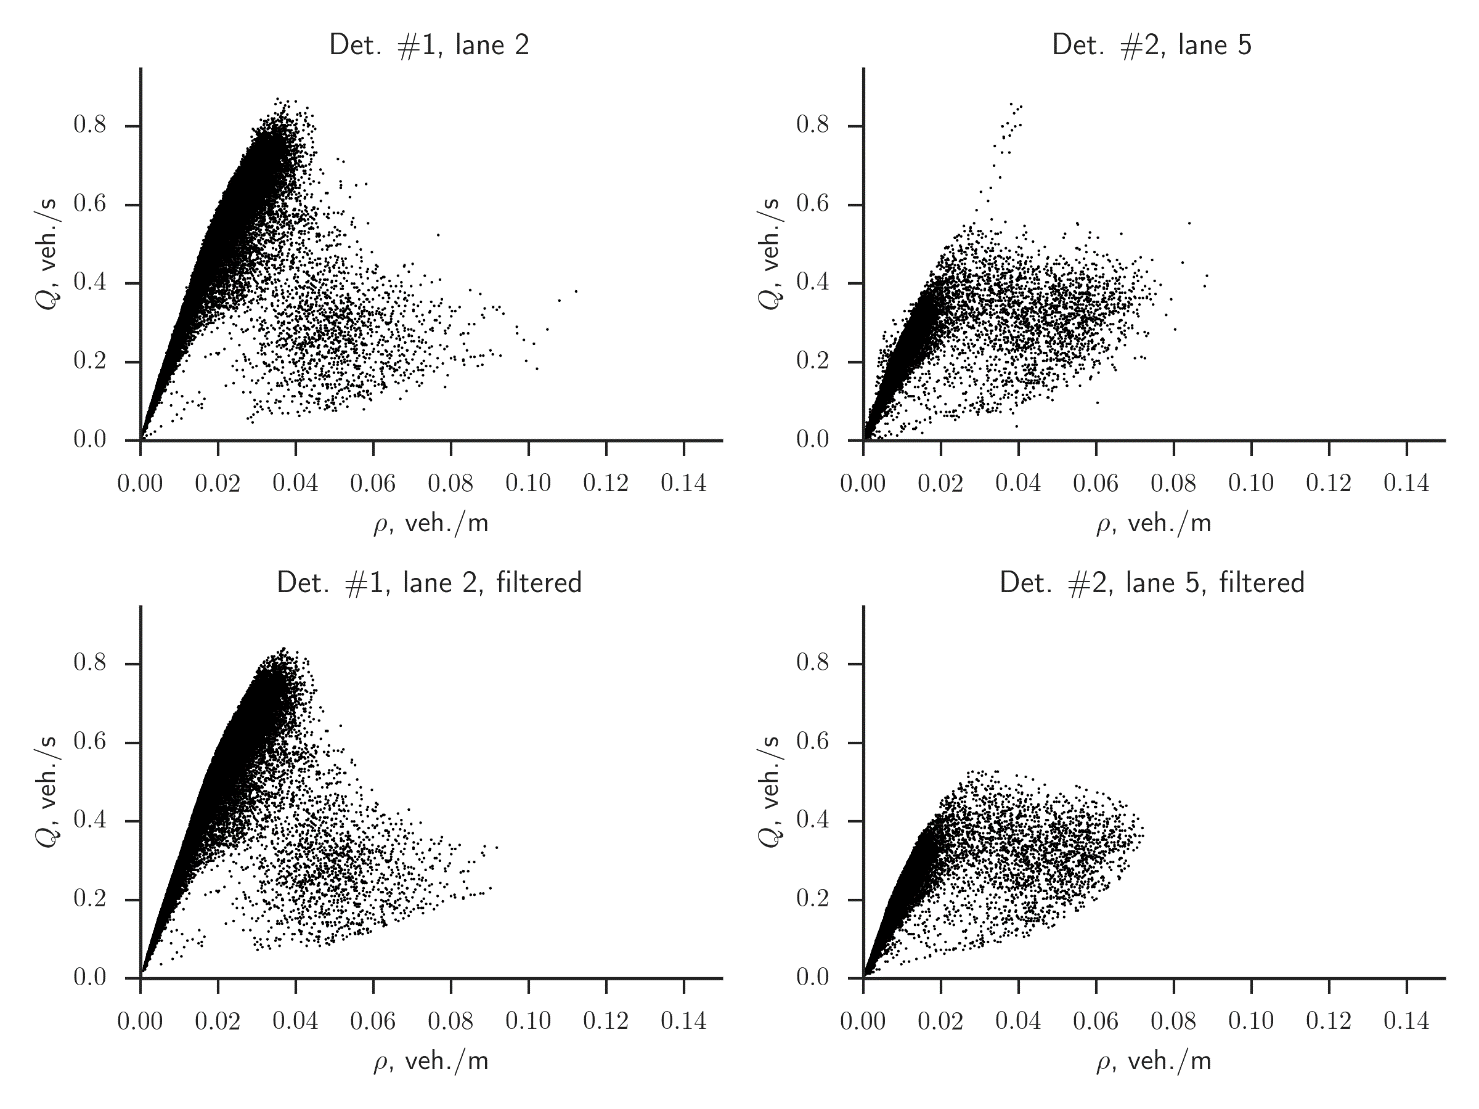
\includegraphics[width=1\linewidth]{detectors_data_alpha.png}
\caption{Экспериментальные данные с двух детекторов, установленных на различных полосах МКАД --- замеренные интенсивности транспортного потока \(Q(\rho)\)[АТС/с] при различной плотности [АТС/м]. Данные представлены за 2012 г. В количестве 288 измерений за день. Сверху исходные данные, снизу отфильтрованные с использованием алгоритма построения выпуклых оболочек.}
\label{fig:detectors_data_alpha}
\end{center}
\end{figure}
В соответствии с теорией трёх фаз транспортного потока Б.С. Кернера на скоростных автомагистралях~\cite{kerner2009introduction} кратко изложенной в разделе~\cref{subsec:ch1/sec4_kerner} выделяем три фазы транспортного потока:
\begin{enumerate}
  \item Свободный поток \(Q(0\leq\rho\leq\rho_1)\)
  \item Синхронизованный поток \(Q(\rho_1\leq\rho\leq\rho_2)\)
  \item Заторный поток \(Q(\rho_1\leq\rho\leq\rho_*)\)
\end{enumerate}
Для каждой из фаз транспортного потока задаём её собственную функциональную зависимость \(Q(\rho)\), сшивая их в точках фазового перехода:
\begin{enumerate}
  \item Свободный поток \(Q(\rho) = \alpha_2\rho^2 + \alpha_1\rho,\ 0\leq\rho\leq\rho_1\)
  \item Синхронизованный поток \(Q(\rho) = \beta_2\rho^2 + \beta_1\rho + \beta_0,\ \rho_1\leq\rho\leq\rho_2\)
  \item Заторный поток \(Q(\rho) = c_*(\rho_*-\rho),\ \rho_1\leq\rho\leq\rho_*\)
\end{enumerate}
Коэффициенты функциональных зависимостей находим, приравнивая значения функций в найденных точках к значениям интенсивностей в них, в результате получаем следующую систему уравнений:
\begin{displaymath}\left\{
\begin{array}{llllll}
  \alpha_2\rho_0^2 + \alpha_1\rho_0 = Q(\rho_0)\\
  \alpha_2\rho_1^2 + \alpha_1\rho_1 = Q(\rho_1)\\
  \beta_2\rho_1^2 + \beta_1\rho_1 + \beta_0 = Q(\rho_1)\\
  \beta_2\rho_2^2 + \beta_1\rho_2 + \beta_0 = Q(\rho_2)\\
  2\beta_2\rho_1 + \beta_1 = c_1 = \left.\frac{\partial Q(\rho)}{\partial \rho}\right|_{\rho = \rho_1}\\
  c_*(\rho_*-\rho_2) = Q(\rho_2)
\end{array} \right.
\end{displaymath}
Осталось только понять чему будет равна производная функции после прохождения критической точки: $\left.\frac{\partial Q(\rho)}{\partial \rho}\right|_{\rho = \rho_1} = c_1 = ?$.
Из экспериментальных наблюдений мы знаем, что после её прохождения интенсивность транспортного потока заметно падает. Это означает, что поток начинает тормозиться, поэтому логично предположить, что $c_1$ есть скорость волны торможения и её можно найти, построив пространственно-временную структуру или карту значений скорости транспортного потока для соответствующих участков автострады (см рис.~\ref{fig:cstart}).

Отметим, что для построения пространственно-временной структуры транспортного потока зачастую недостаточно одних лишь дорожных датчиков, так как они расположены по автомагистрали с недостаточной плотностью.
Тут важную роль играют GPS-треки.
Их ключевой недостаток заключается в том, что GPS фиксирует движение только некоторой доли автомобилей из общего потока.
Доля эта может меняться как в зависимости от фазы потока (плотности движения АТС) так и от времени суток.
Характеристики этой зависимости зачастую связаны с характером источника данных.
Так, например, службы такси будут иметь лучшее покрытие в то время, когда число заказов наибольшее.
Однако, этот недостаток никак не влияет на измеряемую с помощью GPS-треков скорость автомобилей, что позволяет без каких либо ограничений использовать эти данные для построения фундаментальной диаграммы.
\begin{figure}[ht]
\begin{center}
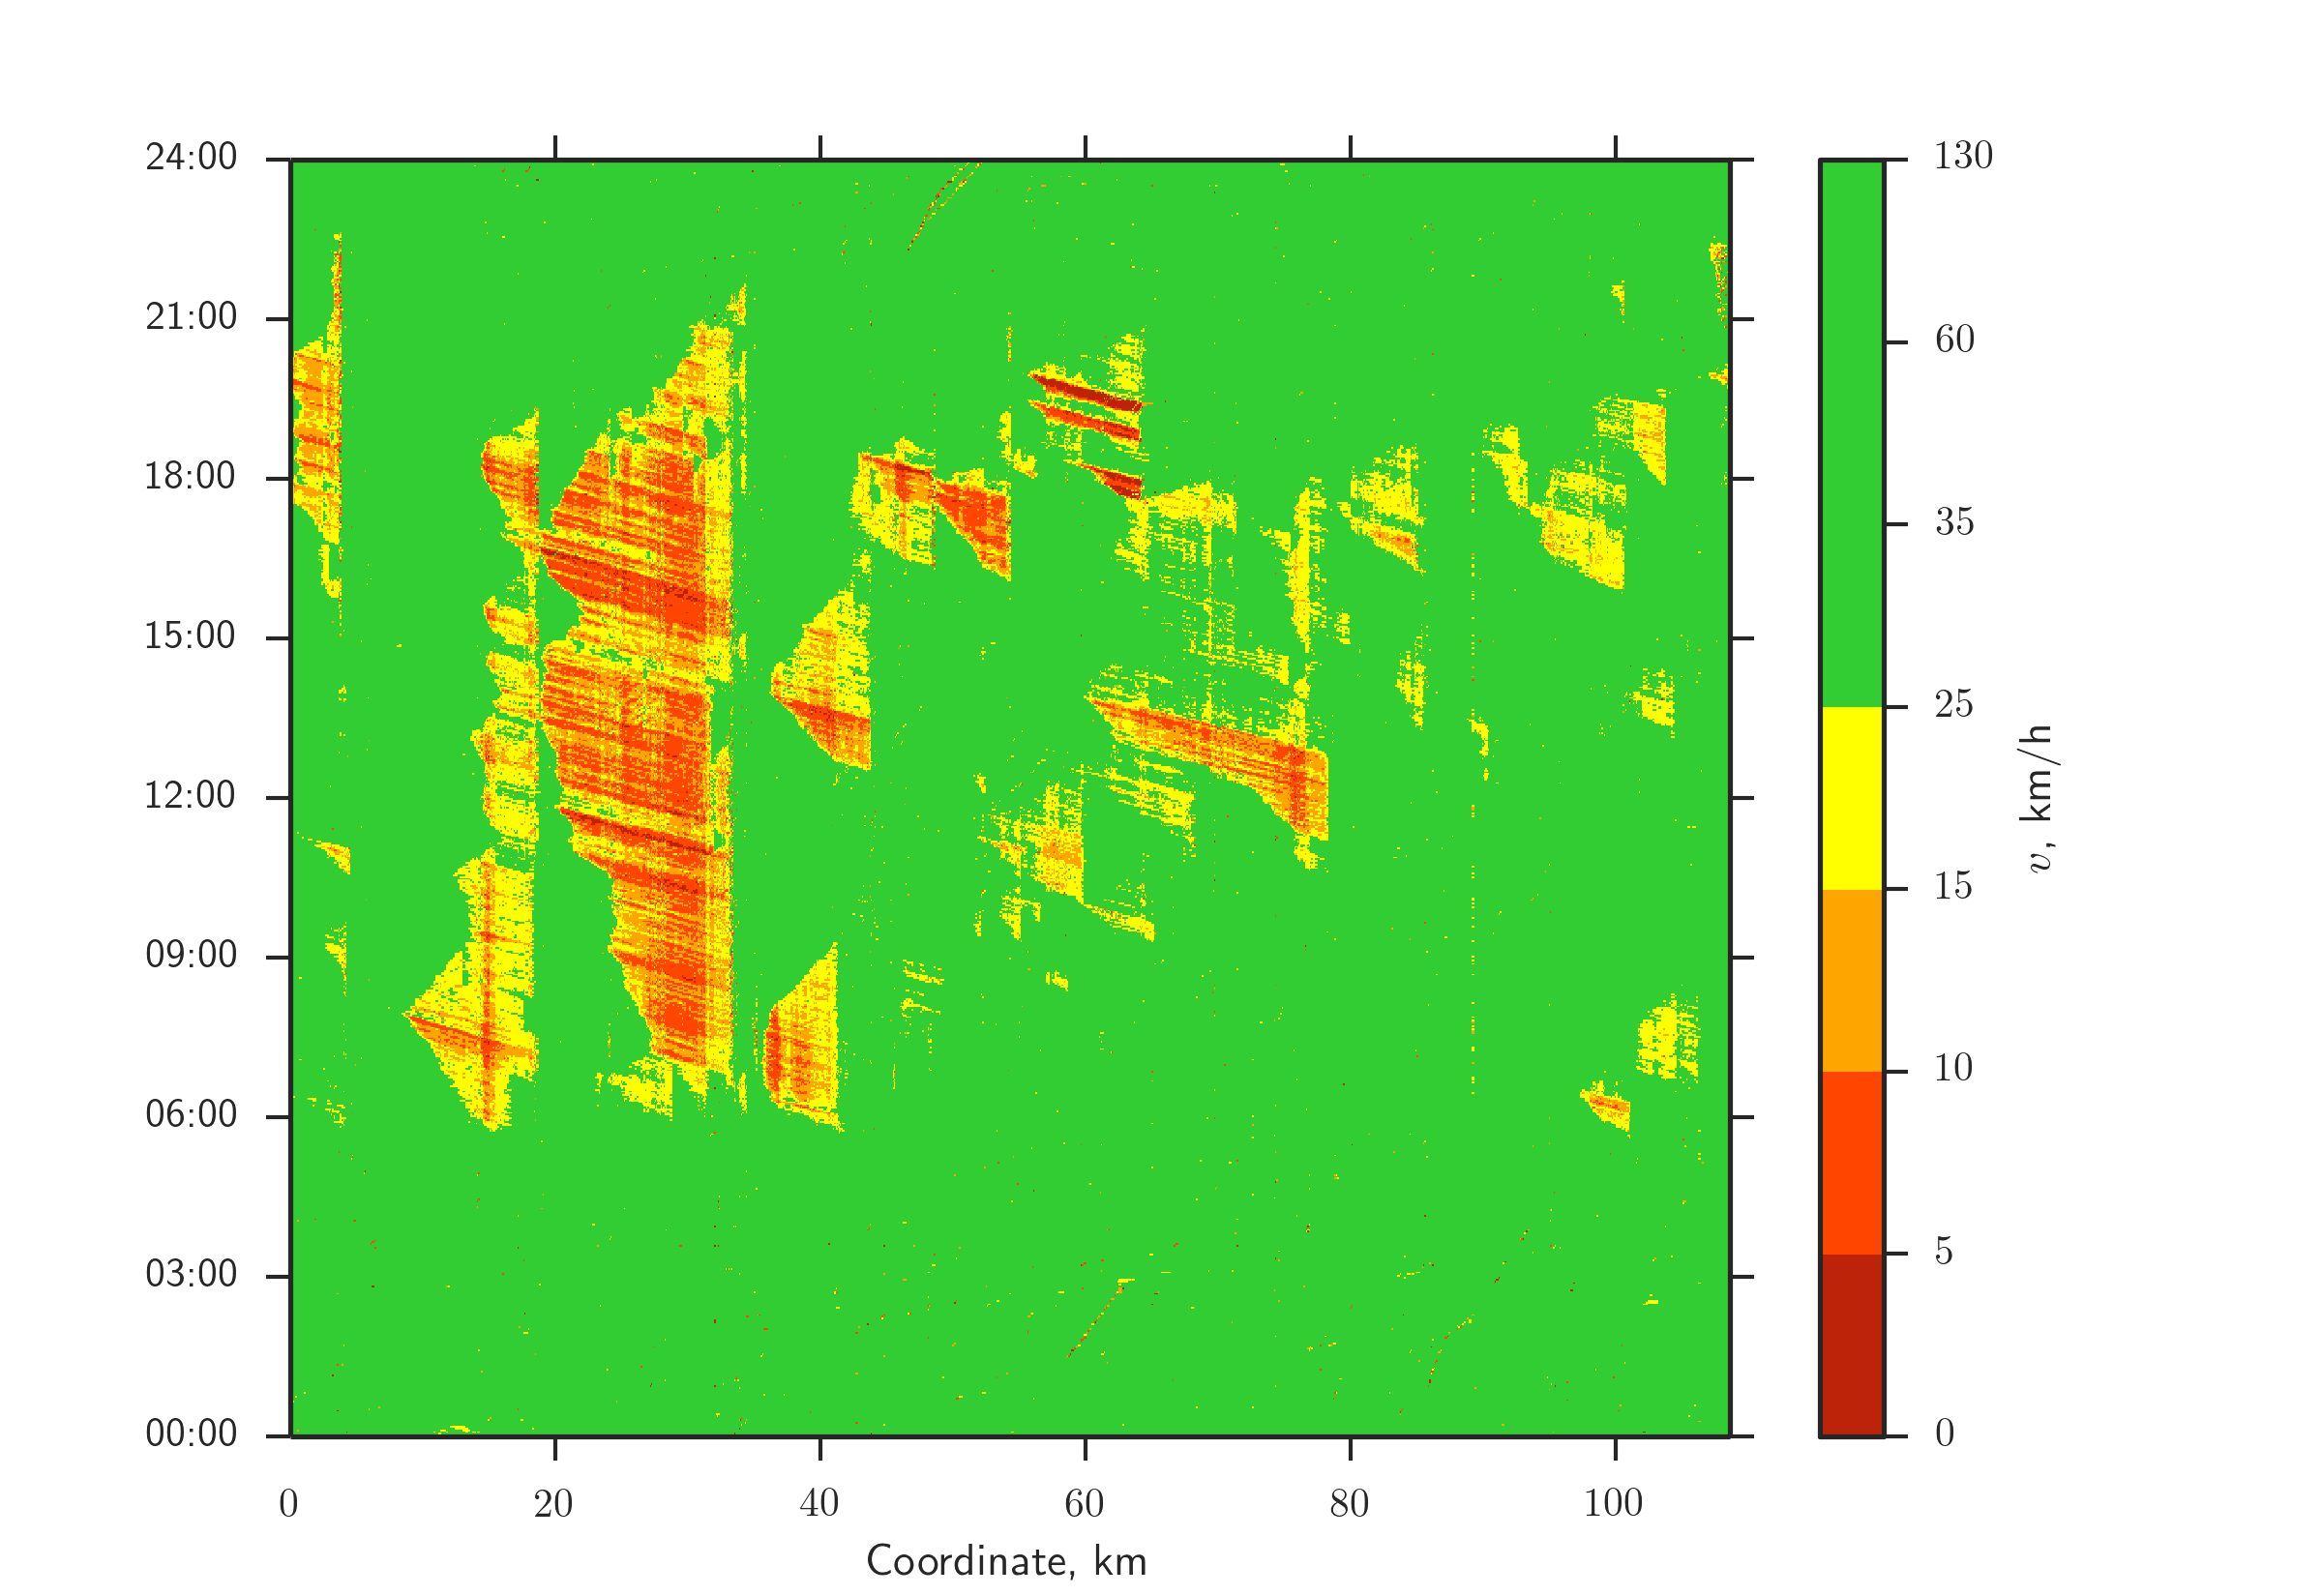
\includegraphics[width=1\linewidth]{c_start.png}
\caption{Пространственно-временная структура значений скорости транспортного потока на внешней стороне МКАД для одного рабочего дня --- 5 декабря 2012 г.}
\label{fig:cstart}
\end{center}
\end{figure}


На рисунке~\ref{fig:cstart} хорошо видны красные линии распространения волн торможения навстречу движению транспортного потока. 
Наклон этих линий, которые со временем остаются параллельными, и есть значение скорости волны торможения. 
Следующая проблема, которую предстоит решить, это как автоматизировать процесс нахождения значений скорости волн торможения по карте скоростей для заданного участка дороги. 
Эта задача была решена с использованием алгоритмов компьютерного зрения~\cite{bradski2000dr} в три этапа~\ref{fig:cend}:
\begin{enumerate}
  \item Выделение границ методом Кэнни~\cite{canny1986computational} --- рис.~\ref{fig:cend}(cлева)
  \item Поиск отрезков среди выделенных границ методом Хафа~\cite{matas2000robust}  --- рис.~\ref{fig:cend}(центр)
  \item Отсеивание ложных линий  --- рис.~\ref{fig:cend}(cправа)
\end{enumerate}
\begin{figure}[ht]
\begin{center}
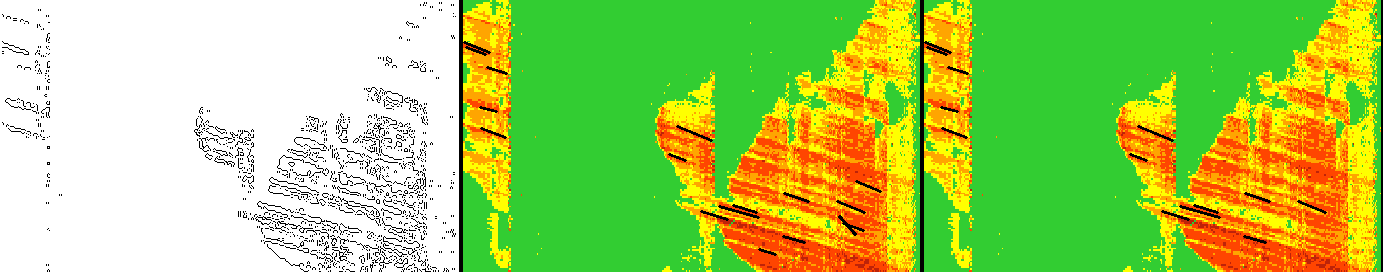
\includegraphics[width=1\linewidth]{c_end.png}
\caption{Нахождение значений скорости волн торможения на пространственно-временной структуре значений скорости транспортного потока на внешней стороне МКАД}
\label{fig:cend}
\end{center}
\end{figure}


Как результат этой работы, была получена гистограмма значений скоростей волны торможения транспортного потока на внешней стороне МКАД~\ref{fig:chist} за 2012 г.

\begin{figure}[ht]
\begin{center}
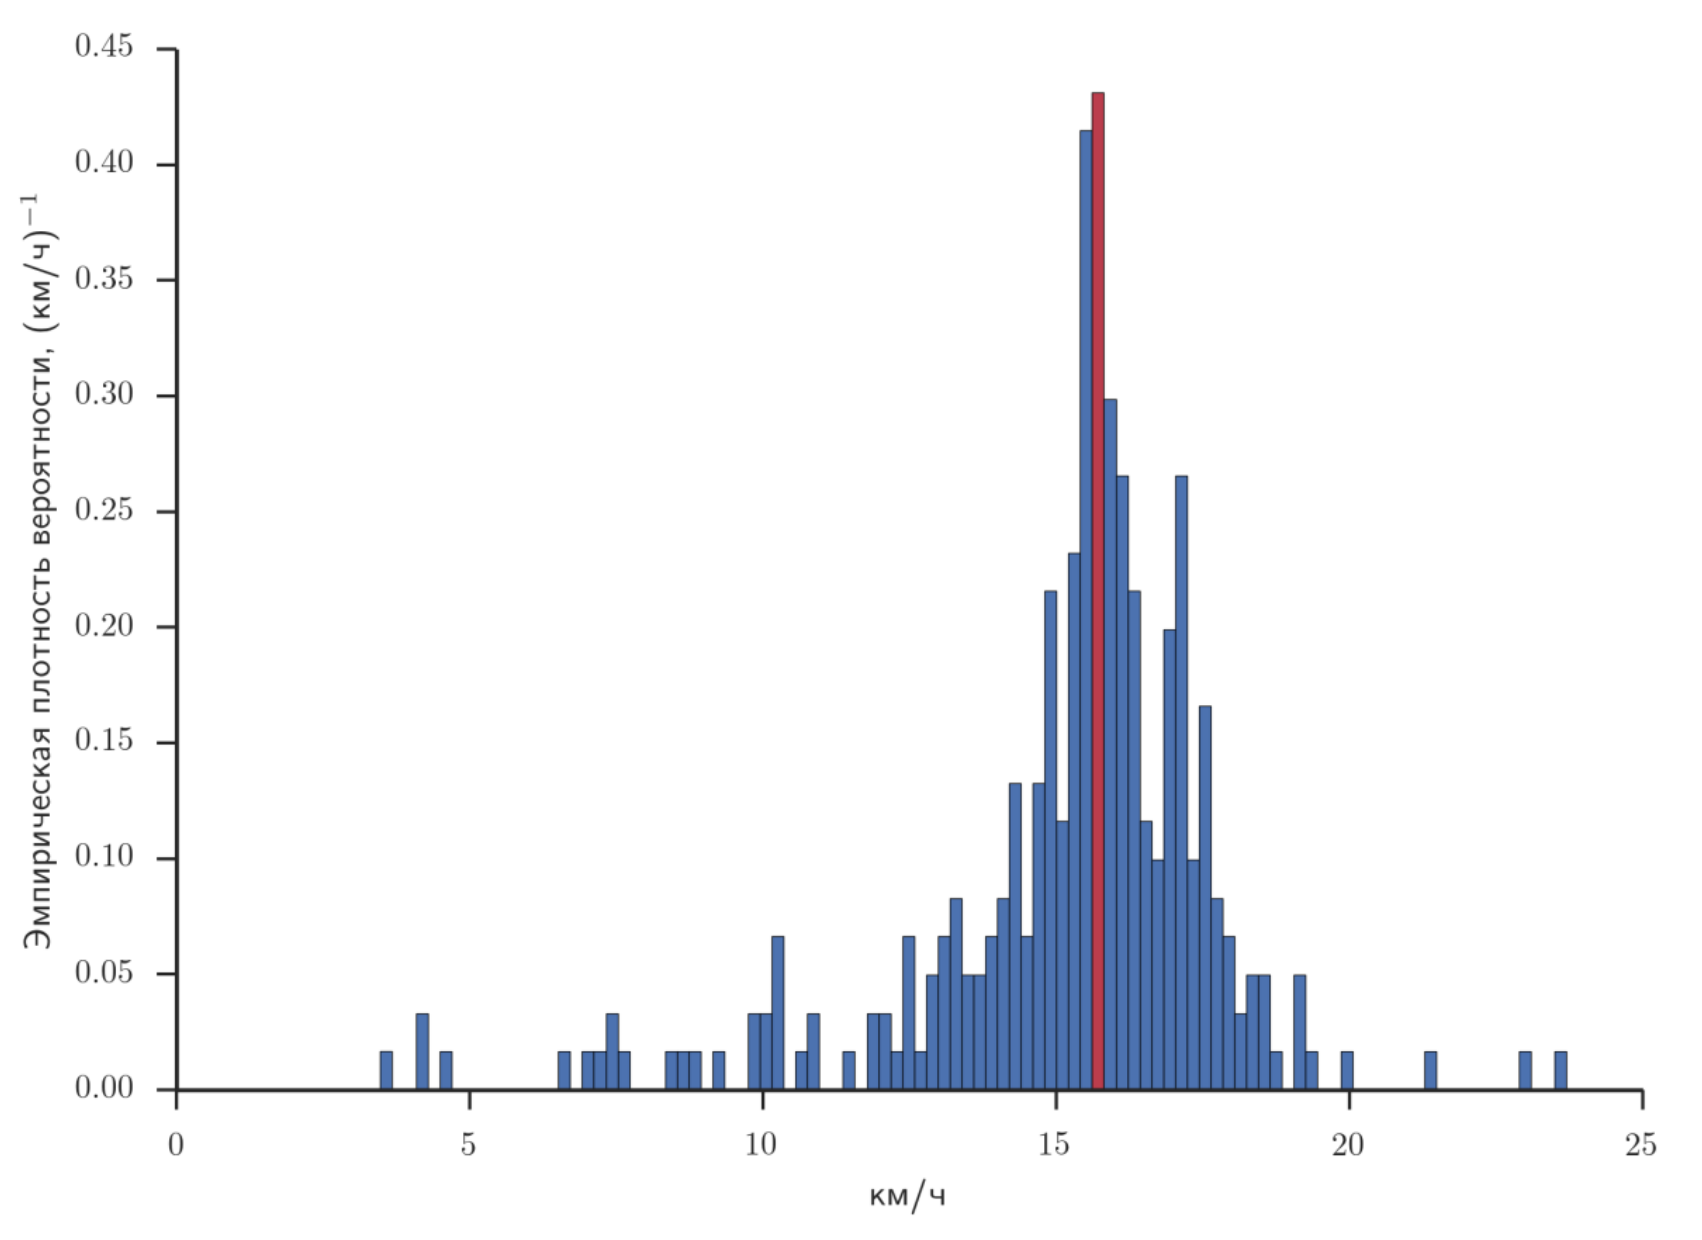
\includegraphics[width=0.9\linewidth]{chist_speed_wave.png}
\caption{Гистограмма значений скоростей волны торможения транспортного потока на МКАД за 2012 г}
\label{fig:chist}
\end{center}
\end{figure}
Отсеяв ложные значения, мы установили, что скорость волны торможения на МКАД \(\left.\frac{\partial Q(\rho)}{\partial \rho}\right|_{\rho = \rho_1} = c_1 = -15.8\) [км/ч], также мы выяснили, что она не зависит от времени года, дня недели и определяется исключительно геометрией дороги.
Данная скорость очень близка к скорости приводимой Кернером~\cite{kerner2009introduction} как скорость <<заднего фронта широко движущегося кластера>>: \(v_g \approx -15\) [км/ч].
Таким образом, в отсутствии достаточно объёмных данных о скорости движения АТС, к чему зачастую ведет отсутствие данных с GPS-треков, можно использовать скорость в -15 [км/ч].

Полученные в итоге примеры фундаментальных диаграмм представлены на рис.~\ref{fig:qresult}
\begin{figure}[ht]
\begin{center}
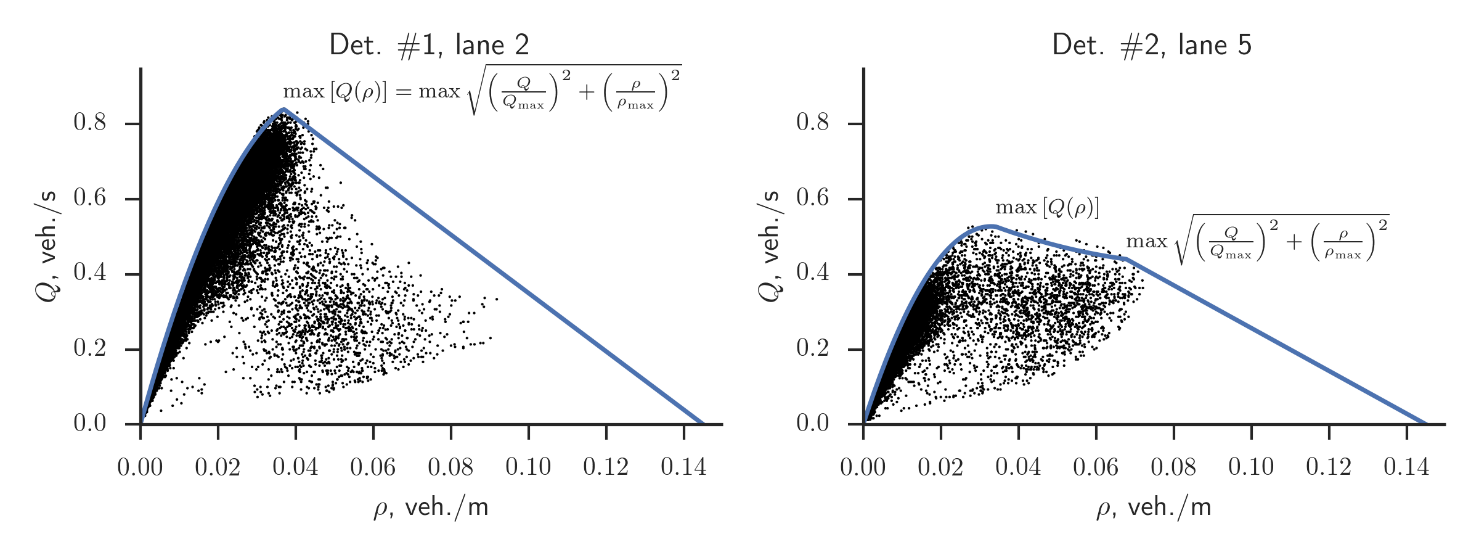
\includegraphics[width=1\linewidth]{Q_result.png}
\caption{Фундаментальные диаграммы для двух разных участков МКАД. Слева для данных со второй полосы (детектор № 1), справа с пятой полосы (детектор №2)}
\label{fig:qresult}
\end{center}
\end{figure}

\FloatBarrier
           % Глава 2
\chapter{Описание математической модели}\label{ch:ch3}

В данном разделе приводится полное математическое описание предлагаемой мезоскопической модели с описанием процедуры моделирования автомагистрали с ее использованием.
\section{Структура модели}
\label{sec:model}
\subsection{Внутренние свойства модели}
\label{sec:graph_structure}
Транспортная сеть представляет собой связный ориентированный граф \(\mathbf{G} = (\mathbf{V}, \mathbf{E})\),
где \(\mathbf{V}\) - множество вершин, \(\mathbf{E} = \{(i, j)\}\) - множество ветвей графа.
На граф также накладываются ограничения на максимальную и минимальную степень вершин \(d(i)$: $\min(d(i)) = 1\) и~\(\max(d(i)) = 3\).
Также \(\forall i: d(i) > 1 \rightarrow \exists j, l \in \mathbf{V} : (j, i), (i, l) \in \mathbf{E}\), т.е. не существует вершины, в которой только заканчиваются несколько ветвей, и не существует вершины, в которой только начинаются несколько ветвей.

Определим теперь все типы вершин графа в зависимости от их степеней.
\begin{enumerate}
  \item \(d(i) = 1\). В данном случае существует два варианта:
  \begin{enumerate}
    \item \(i:\ \exists (i,j)\in \mathbf{E}\). Такие вершины будем называть \emph{вершинами-въездами}. Вершины въезды образуют множество \(\mathbf{V}_\text{in}\) и являются источниками автомобильно-транспортных средств(АТС) в рассматриваемой модели.
    \item \(i:\ \exists (j,i)\in \mathbf{E}\). Такие вершины будем называть \emph{вершинами-съездами}. Вершины съезды образуют множество \(\mathbf{V}_\text{out}\) и являются стоками автомобилей в рассматриваемой модели.
  \end{enumerate}
  \item \(d(i) = 2\). Это внутренние вершины модели образующие множество \(\mathbf{V}_\text{int}\).
  \item \(d(i) = 3\)~--- вершины-центры перекрестков дорожно-транспортной сети. Данные вершины также входят в множество \(\mathbf{V}_\text{int}\), но образуют еще два подмножества.
  \begin{enumerate}
    \item Если \(\exists (i, j) \in \mathbf{E},\ (i, k) \in \mathbf{E} : j\neq k \), то такие вершины образуют множество \(\mathbf{V}_\text{sep}\)~--- вершины в которых происходит разделение потоков в дорожно-транспортной сети.
    \item Если \(\exists (j, i) \in \mathbf{E},\ (k, i) \in \mathbf{E} : j\neq k \), то такие вершины образуют множество \(\mathbf{V}_\text{mer}\)~--- вершины, в которых происходит слияние потоков в дорожно-транспортной сети.
  \end{enumerate}
\end{enumerate}
Таким образом, \(\mathbf{V} = \mathbf{V}_\text{int} \cup \mathbf{V}_\text{out} \cup \mathbf{V}_\text{in}\)~--- все вершины распределены по трем непересекающимся группам. Вершины же перекрестки с \(d(i) = 3\) дополнительно разделены по типу перекрестка причем \(V_\text{sep}\bigcap V_\text{mer} = \emptyset\). Ввиду того, что в данной работе рассматриваются только автомагистрали, то вершины с \(d(i) = 4\) и более не встречаются.

Разделим схожим образом ребра инцидентные этим вершинам. Рассмотрим для этого некоторое ребро \((i,j)\).
\begin{enumerate}
  \item Если \(i\in \mathbf{V}_\text{in}\), то ребро \((i,j)\)~--- это ребро-въезд. Такие ребра образуют множество въездов \(\mathbf{E}_\text{in}\).
  \item Если \(j\in \mathbf{V}_\text{out}\), то ребро \((i,j)\)~--- это ребро-съезд. Такие ребра образуют множество съездов \(\mathbf{E}_\text{out}\).
  \item Если \(i\in \mathbf{V}_\text{int}\) и \(j\in \mathbf{V}_\text{int}\), то ребро \((i,j)\)~--- это внутреннее ребро модели. Такие ребра образуют множество внутренних ребер модели \(\mathbf{E}_\text{int}\).
\end{enumerate}
Также как и с вершинами \(\mathbf{E} = \mathbf{E}_\text{int} \cup \mathbf{E}_\text{out} \cup \mathbf{E}_\text{in}\) за исключением случая, когда модель представляет из себя одно ребро, который в этой работе не рассматривается.

Определим теперь понятие состояния модели в момент времени \(t\).
Для этого нам понадобится понятие автомобильной группы на ветви \((i, j): \mathbf{A}^t_k = \{\mathrm{Pos}_k, V_k, N_k\}\), обладающей следующими характеристиками:
\begin{enumerate}
    \item \(\mathrm{Pos}_k\)~--- позиция начала группы относительно начала ветви, на которой она расположена.
    \item \(V_k\)~--- скорость группы АТС.
    \item \(N_k\)~--- размер группы АТС из \(\mathbb{R}_{\geq 0} = \mathbb{R}_+\).
\end{enumerate}

Пусть теперь \(\mathbf{A}^t_{i,j} = \{\mathbf{A}^t_k\}\)~--- упорядоченное множество автомобильных групп на ветви \((i,j)\). Причем \(\forall l, m: l<m \rightarrow \mathrm{Pos}_l > \mathrm{Pos}_m\)~--- группы не могут обгонять друг друга.

Таким образом, введем состояние системы в момент времени \(t\) как \(\mathbf{A}^t = \{\mathbf{A}^t_{i,j}\} \cup \{A^t_{\text{out}, i, j}\}\), т.е. положение, скорость, размер и тип всех автомобильных групп на всех ветвях дорожно-транспортной сети. 
Группы АТС \(\{A^t_{\text{out}, i, j}\}\) представляют собой специальные группы-буферы. Их особые свойства рассматриваются в разделе Общих свойств модели.

Для расчетов нам также понадобится понятие потенциала трансфера \(\text{Tr}_{(i, j), k}^t (\mathbf{A}^t, \mathbf{A}^{t-1})\)~--- число АТС, которые могут съехать с ветви \((i,j)\) на ветвь \((j,k)\) в интервал времени от \(t-1\) до \(t\). 
Данная величина вычисляется заново на каждой временной итерации в зависимости от состояния системы.


\subsection{Внешние свойства модели}
\label{sec:graph_structure}
Определим теперь свойства модели задаваемые при ее инициализации.

Рассмотрим предварительно три ветви с \(d(j) = 3:\ (i, j), (j, k_1), (j, k_2)\). 
В данной работе мы считаем \((j, k_1)\) продолжением автомагистрали, а \((j, k_2)\)~--- съездом с нее. Данное распределение полностью задается в момент инициализации модели.

Перечислим все внешние параметры модели для каждой ветви \((i, j) \in \mathbf{E}\) графа \(\mathbf{G}\).
\begin{enumerate}
    \item Длина ветви \(l_{i, j}\).
    \item Число полос, по которым разрешено движение автомобилей по данной ветви \(n_{i, j}\).
    \item \(I_{i, j} = \{0, 1\}\)~--- идентификатор того, является ветвь съездом или нет. Если является, то \(I_{i, j} = 1\).
    \item Функция скорости для данной ветви \(V = f_{i,j}(\rho)\), \(f_{i,j}: \mathbb{Q}_+ \rightarrow \mathbb{Q}_+\), где \(\rho\in\mathbb{R}_+\)~--- плотность АТС.
        В данной работе рассматриваются только ограниченные непрерывные монотонно убывающие функции скорости.
        Процедура получения данной функции из экспериментальных данных детально описана в разделе~\ref{ch:ch2}.
    \item Матрица перемешивания в узле \(j\) в момент времени \(t\), задаваемая функцией \(M_j(t)\).
        В случае если \(j: \nexists (j,k) \in \mathbf{E}_\text{out} \rightarrow \forall t: M_j(t) = 0\).
    \item Интенсивность источника в узле \(i\) в момент времени \(t\), задаваемая функцией \(F_i(t)\). Для всех \(i: i\notin \mathbf{V}_\text{in} \rightarrow \forall t: F_i(t) == 0\).
\end{enumerate}

Также у каждой ветви есть буфер АТС \(A^t_{\text{out}, i, j} = \{\mathrm{Pos}_{\text{out}, i, j}, V_{\text{out}, i, j}, N_{\text{out}, i, j}\}\), представляющий из себя группу АТС с \(\mathrm{Pos}_{\text{out}, i, j} = l_{i, j},\ V_{\text{out}, i, j} = 0\). 
Данная группа моделирует очередь на съезд с ребра \((i, j)\)~--- т.е. группу \((j, k)\) с \(I_{i, j} = 1\). 
Работа с данной группой детально описана в разд. 
Алгоритмов перемещения и объединения групп АТС~\ref{sec:calc_functions}.

Будем считать, что в модели все автомобили имеют фиксированный размер \(L_\text{car}^\text{avg}\).
В дальнейшем, путем изменения этой величины можно также исследовать зависимость поведения автомагистрали от состава потока автомобилей.
С его помощью получаем максимальное число автомобилей на ветви \((i,j)\) как \(N^{i,j}_\text{max} = \frac{l_{i,j} \cdot n_{i, j}}{L_\text{car}^\text{avg}}\).

Введем также понятие динамического размера автомобилей \(L_\text{car}(V) = L_\text{car}^\text{avg} + a\cdot V\), где \(a = 0.504\). 
Данная величина отражает тот факт, что автомобили в среднем на определенной скорости не сближаются сильнее некоторого расстояния. 
Сама же константа \(a\), как и данное приближение, взята из книги~\cite{gasn2017introd}.
Видно, что данное соотношение~--- это соотношение из модели Танака~\ref{subsec:ch1/sec1/sub2} без квадратичного члена отвечающего за влияние аномальных погодных условий (дождь, снег).

Таким образом, получаем, что все характеристики автомобильной группы ограничены сверху.
\begin{enumerate}
  \item Положение \(\mathrm{Pos}_k\) группы АТС длиной ветви на которой группа находится.
  \item Скорость \(V_k\) ограничена максимальной скоростью на ветви, которую можно определить из функции скорости $f_{i,j}(\rho)$.
  \item Максимальный размер \(N_k\) ограничен максимальным числом автомобилей на ветви \(N^{i,j}_\text{max}\).
\end{enumerate}

Однако поскольку в нашей модели все группы АТС движутся так, как будто каждый автомобиль в группе обладает полным знанием обо всех других автомобилях, то это накладывает на группы логическое ограничение на их размер, так как сложно ожидать такого поведения у АТС в огромной группе. 
Мы в данной работе считаем разумным ограничение в \(N_\text{max} = 20\) АТС.

Также нам понадобится величина среднего ускорения группы АТС \(a_\text{avg}\) для ограничения увеличения скорости движения групп АТС по ветвям автомагистрали. 
В данной работе величина ускорения взята за константу и равна \(2.2\ \text{м/c2}\) (см.~\cite{long2000acceleration}).


\section{Алгоритмы перемещения и объединения групп АТС}
\label{sec:calc_functions}
Определим как группы АТС объединяются в одну, как переезжают с одной ветви на другую, как движутся по ветви и как съезжают на ветви-съезды.
Также определим функцию расчета \(\text{Tr}_{(i, j), k}^t (\mathbf{A}^t, \mathbf{A}^{t-1})\) на каждом временном шаге.

\subsection{Движение групп АТС по ветви}
На каждой итерации алгоритма надо рассчитать новое положение групп АТС для каждой ветви.
Перерасчет положения групп а также их скорости производит функция \(\text{group\_mover}(\mathbf{A}^t_{i,j},\ k,\ (i,j),\ \tau,\ t)\) по алгоритму~\ref{group_mover}.
Расчеты по данному алгоритму сводятся к следующим шагам.
\begin{enumerate}[leftmargin=2.05cm,label=Шаг \arabic*.,ref=\arabic*]
  \item Для выбранной группы АТС \(\mathbf{A}^t_k$ на ветви $(i,j)\) рассчитываем ее скорость \(V_k'\) на основании плотности автомобилей на участке автодороги перед ней.
  \item Рассчитываем новое положение группы АТС.
  \item Если группа оказалась в конце ветви:
  \begin{enumerate}
    \item рассчитать сколько времени она ехала до конца ветви;
    \item в соответствии с матрицей перемешивания часть группы добавляется в буфер-группу \(A^t_{\text{out}, i, j}\);
    \item оставшаяся часть группы \(\mathbf{A}^t_k\) пытается переехать на следующую для нее ветвь с \(I_{j, m_1} = 0\);
    \item группа-буфер \(A^t_{\text{out}, i, j}\) пытается переехать на следующую для нее ветвь с \(I_{j, m_1} = 1\).
  \end{enumerate}
\end{enumerate}

\begin{algorithm}[!ht]
    \caption{Алгоритм расчета положения и скорости группы АТС}
    \label{group_mover}
    \begin{algorithmic}
        \REQUIRE \(\mathbf{A}^t_{i,j}\)~--- множество характеристик автомобильных групп на ветви; \\
                 \(k\)~--- индекс рассматриваемой автомобильной группы; \\
                 \((i,j)\)~--- рассматриваемая ветвь графа; \\
                 \(\tau\)~--- временной шаг; \\
                 \(t\)~--- текущий момент времени;
        \IF {\(\mathrm{Pos}_k = l_{i,j}\)}
            \STATE Если группа АТС уже в конце ветви то она просто пытается переехать на следующую ветвь
            \STATE Пусть \(j' : (j, j') \in \mathbf{\widetilde{E}}$~--- ветвь c $I_{j, j'} = 0\)
            \STATE \(\text{group\_transferrer}(\mathbf{A}^t,\ \mathbf{A}^{t-1},\ k,\ (i,j),\ (j,j'),\ \tau')\) из Алгоритма~\ref{group_transferrer}
            \RETURN 0
        \ENDIF
        \STATE \(\mathrm{Pos}_k += V_k \cdot \tau\)
        \STATE Пусть \(\rho = \frac{\sum_{m=k+1}^{\text{len}(\mathbf{A}^t_{i,j})} N_m}{l_{i,j} \cdot n_{i,j}}\)~--- плотность АТС на участке ветви \((i,j)\) перед группой АТС \(k\), тогда \(V_k' = f_{i,j}(\rho)\)~--- новая скорость группы АТС.
        \IF {\(V_k' - V_k > a_\text{avg} \cdot \tau\)}
            \STATE \(V_k' = V_k + a_\text{avg} \cdot \tau\)
        \ENDIF
        \IF {\(\mathrm{Pos}_k \geq l_{i,j}\) и \(k = 0\)}
            \STATE \(\tau' = \tau \cdot \frac{\mathrm{Pos}_k - l_{i,k}}{V_k \cdot \tau}\)~--- 'оставшееся' время движения автомобильной группы
            \STATE \(\mathrm{Pos}_k = l_{i,k}\)
            \STATE Добавим АТС в группу-буфер \(\mathbf{A}^t_{\text{out}, i, j}\)
            \STATE \(N_{\text{out}, i, j} += N_k \cdot M_j(t)\)
            \STATE \(N_k = N_k \cdot (1 - M_j(t))\)
            \STATE Оставшиеся АТС должны продолжить движение по магистрали
            \STATE Пусть \(j' : (j, j') \in \mathbf{\widetilde{E}}\)~--- ветвь c \(I_{j, j'} = 0\)
            \STATE \(\text{group\_transferrer}(\mathbf{A}^t,\ \mathbf{A}^{t-1},\ k,\ (i,j),\ (j,j'),\ \tau')\) по Алгоритму~\ref{group_transferrer}
            \STATE Группа-буфер пытается съехать
            \STATE Пусть \(j'' : (j, j'') \in \mathbf{\widetilde{E}}\)~--- ветвь c \(I_{j, j''} = 0\)
            \STATE \(\text{group\_transferrer}(\mathbf{A}^t,\ \mathbf{A}^{t-1},\ k,\ (i,j),\ (j,j''),\ \tau')\) по Алгоритму~\ref{group_transferrer}
        \ELSE
            \IF {\(\mathrm{Pos}_k \geq \mathrm{Pos}_{i,k-1}\)}
                \STATE \(\mathrm{Pos}_k = \mathrm{Pos}_{k-1} - L_\text{car}(V_{k-1}) \cdot N_{k-1}\)
            \ENDIF
            \STATE \(\text{group\_union}(\mathbf{A}_{i,j},\ k,\ (i,j),\ t)\)
        \ENDIF
        \STATE Если группа АТС \(\mathbf{A}^t_k\) все еще существует \(V_k = V_k'\)
    \end{algorithmic}
\end{algorithm}

Заметим, что функция \(\text{group\_transferrer}\)~алгоритм~3 вызывается тут с временным шагом \(\tau'\), что означает что группа АТС при переезде на новую ветвь будет двигаться меньшее количество времени.


\subsection{Объединение двух групп АТС}
После изменения положения группы АТС на ветви нужно проверить не может ли она быть объединена с какой либо другой группой.
Поскольку группы движутся только вперед и в нашей модели не могут обгонять друг друга, то проверка на возможность
объединения идет только с группой перед рассматриваемой.
То есть для группы АТС \(j\) рассматривается возможность ее слияния с группой \(j-1\).
За слияние групп отвечает функция \(\text{group\_union}(\mathbf{A}^t_{i,j},\ k,\ (i,j),\ t)\), работающая по алгоритму~\ref{group_union}.

\begin{algorithm}[!ht]
    \caption{Алгоритм объединения групп АТС}
    \label{group_union}
    \begin{algorithmic}
        \REQUIRE \(\mathbf{A}^t_{i,j}\)~--- множество характеристик автомобильных групп на ветви; \\
                 \(k\)~--- индекс рассматриваемой автомобильной группы; \\
                 \((i,j)\)~--- рассматриваемая ветвь графа; \\
                 \(t\)~--- текущий момент времени;
        \IF{\(k = 0\)}
            \STATE Группу не с чем объединять так как она самая первая
        \ELSE
            \IF{\(\mathrm{Pos}_{k-1} - \mathrm{Pos}_k \leq L_\text{car}(V_{k-1}) \cdot N_{k-1}$ и $N_{k-1} + N_k \leq N_\text{max}\)}
                \STATE Объединяем группы в одну
                \IF{\(k - 1 = 0\) и \(\mathrm{Pos}_(k - 1) = l_{i,j}\)}
                    \STATE \(N^{j}_\text{exit} += N_k \cdot M_j(t)\)
                    \STATE \(N_{k-1} += N_k \cdot (1 - M_j(t))\)
                \ELSE
                    \STATE \(N_{k-1} += N_k\)
                \ENDIF
                \STATE \(\text{del} \mathbf{A}^t_k\)~--- группа \(k\) удаляется
            \ENDIF
        \ENDIF
    \end{algorithmic}
\end{algorithm}


\subsection{Перемещение групп АТС между ветвями}
Когда группа автомобилей достигает конца ветви, на которой она находится, требуется определить какая ее часть переедет на
следующий сегмент автомагистрали и какое положение и скорость примет на новой ветви.
За данные расчеты отвечает функция \(\text{group\_transferrer}(\mathbf{A}^t,\ \mathbf{A}^{t-1}, k,\ (i,j),\ (j,j'),\ \tau,\ t)\) по алгоритму~\ref{group_transferrer}.
Расчеты по данному алгоритму сводятся к следующим шагам.
\begin{enumerate}[leftmargin=2.05cm,label=Шаг \arabic*.,ref=\arabic*]
  \item Определяем индекс новой группы АТС на ветви \((j,j')\).
  \item Определяем, может ли группа переехать на новую ветвь полностью. Если да:
  \begin{enumerate}
    \item создаем новую группу АТС в конце ветви \((j,j')\) с \(N_{k'} = N_k\).
    \item Удаляем группу \(k\) из \(\mathbf{A}^t_{i,j}\).
  \end{enumerate}
  \item Если нет:
    \begin{enumerate}
    \item создаем новую группу АТС в конце ветви \((j,j')\) с \(N_{k'} = N'\), где \(N'\)~--- число АТС которые могут переехать.
    \item Уменьшаем размер группы \(k\) на величину \(N'\).
  \end{enumerate}
  \item Вызываем функцию для перемещения новой группы по ветви \((j,j')\).
\end{enumerate}

\begin{algorithm}[!ht]
    \caption{Алгоритм перемещения группы АТС на новую ветвь}
    \label{group_transferrer}
    \begin{algorithmic}
        \REQUIRE \(\mathbf{A}^t\)~--- состояние системы в текущий момент времени; \\
                 \(\mathbf{A}^{t-1}\)~--- состояние системы в предыдущий момент времени; \\
                 \(k\)~--- индекс рассматриваемой автомобильной группы; \\
                 \((i,j)\)~--- ветвь с которой хочет съехать группа АТС; \\
                 \((j,j')\)~--- ветвь на которую хочет съехать группа АТС; \\
                 \(\tau\)~--- временной шаг; \\
                 \(t\)~--- текущий момент времени; \\
        \IF {\(N_k \leq \text{Tr}_{(i, j), j'}^t (\mathbf{A}^t, \mathbf{A}^{t-1})\)}
            \STATE Группа полностью может переехать на новую ветвь
            \STATE Пусть \(k' = \text{len}(\mathbf{A}^t_{j,j'}) + 1\)~--- индекс новой группы АТС
            \STATE Создаем новую группу АТС на ребре \((j,j')\) с индексом \(k'\) и характеристиками:
            \STATE \(\mathrm{Pos}_{k'}  = 0,\ V_{k'}  = f_{j,j'}(\rho), N_{k'} = N_k\)
            \STATE Удаляем группу \(k\) из \(\mathbf{A}^t_{i,j}\)
            \STATE \(\text{group\_mover}(\mathbf{A}^t_{j,j'},\ k',\ (j,j'),\ \tau,\ t)\)
        \ELSE
            \STATE Только часть группы переезжает на новую ветвь
            \STATE Пусть \(k' = \text{len}(\mathbf{A}^t_{j,j'}) + 1\)~--- индекс новой группы АТС
            \STATE Создаем новую группу АТС на ребре \((j,j')\) с индексом \(k'\) и характеристиками:
            \STATE \(\mathrm{Pos}_{k'}  = 0,\ V_{k'}  = f_{j,j'}(\rho), N_{k'} = \text{Tr}_{(i, j), j'}^t (\mathbf{A}^t, \mathbf{A}^{t-1})\)
            \STATE \(N_k -= \text{Tr}_{(i, j), j'}^t (\mathbf{A}^t, \mathbf{A}^{t-1})\)
            \STATE \(\text{group\_mover}(\mathbf{A}^t_{j,j'},\ k',\ (j,j'),\ \tau,\ t)\)
        \ENDIF
    \end{algorithmic}
\end{algorithm}

\section{Расчетный цикл}
\label{sec:calc_loop}

\subsection{Расчет потенциала трансфера}
Для начала определим то, как в конце каждой итерации рассчитывается сколько АТС могут переехать с ветви \((i,j)\) на ветвь \((j,k)\).
Особенностью является то, что алгоритм рассчитывает не потенциал трансфера для ветви \((i,j)\) на ветвь \((j,k)\), а все потенциалы трансфера \(\forall i: (i,j)\in \mathbf{E} \rightarrow \text{Tr}_{i, j}^k\).
То есть для ветви \((j,k)\) рассчитываются всевозможные \(\text{Tr}_{i, j}^k\).

Данный расчет производит функция \(\text{Tr\_calculator}(\mathbf{A}^t, \mathbf{A}^{t-1},\ (j,k),\ \tau)\) по алгоритму~\ref{max_transfer_calculation}.
В процессе расчета нам также понадобятся величины \(Q_(i,j) = \text{max}(\rho\cdot f_{i,j}(\rho))\)~--- максимальный поток АТС на ветви \((i,j)\),
\(N^{i,j}_\text{max}\)~--- максимальное число АТС на ветви \((i,j)\) и \(N^t_{i,j} = \sum_{m=0}^{\text{len}(\mathbf{A}^t_{i,j})} N_m\)~--- текущее число АТС на ветви \((i,j)\).

Процедура расчета сводится к определению двух величин:
\begin{enumerate}[label=\arabic*),ref=\arabic*]
  \item \(P_i\)~--- потенциальное количество АТС которые могут доехать до конца ветви \((i,j)\) предшествующей \((j,k)\);
  \item \(N_\text{total}\)~--- сколько всего АТС может переехать на ветвь \((j,k)\) на основании ее вместимости и максимального потока на ней.
\end{enumerate}
В итоге число АТС, которые могут переехать с ветви \((i,j)\) на ветвь \((j,k)\) определяется формулой \(N_\text{total} \cdot \frac{P_i}{\sum P_i}\).


\begin{algorithm}[!hb]
    \caption{Алгоритм расчета \(\text{Tr}_{i, j}^k\)}
    \label{max_transfer_calculation}
    \begin{algorithmic}
        \REQUIRE \(\mathbf{A}^t\)~--- состояние системы в текущий момент времени; \\
                 \(\mathbf{A}^{t-1}\)~--- состояние системы в предыдущий момент времени; \\
                 \((j,k)\)~--- ветвь для которой проводится расчет; \\
                 \(\tau\)~--- временной шаг; \\
        \STATE Пусть \(\mathbf{I} = \{i : (i,j) \in \mathbf{E}\}\)~--- множество ветвей предшествующих рассматриваемой
        \FORALL{\(i \in \mathbf{I}\)}
            \STATE \(P_i = 0\)~--- число АТС которые теоретически могут достигнуть конца их ветви на следующей временной итерации
            \FORALL{\(m=0;\ l\leq \text{len}(\mathbf{A}^t_{i,j});\ m++\)}
                \IF{\(\mathrm{Pos}_m + V_m \cdot \tau \geq m_{i,j}\)}
                    \IF {\((j,k) \in \mathbf{E}_\text{int}\)}
                        \STATE \(P_i += N_m \cdot (1 - M_j(t))\)
                    \ELSE
                        \STATE \(P_i += N_m \cdot M_j(t)\)
                    \ENDIF
                \ENDIF
            \ENDFOR
        \ENDFOR
        \STATE Определим \(N_\text{total}\)~--- сколько всего АТС может переехать на ветвь \((j,k)\)
        \IF {\(N^{j,k}_\text{max} - N^{j,k}_\text{cur} < Q_(j,k)\)}
            \STATE \(N_\text{total} = N^{j,k}_\text{max} - N^{j,k}_\text{cur}\)
        \ELSE
            \STATE \(N_\text{total} = Q_(j,k)\)
        \ENDIF
        \FORALL {\(i \in \mathbf{I}\)}
            \STATE \(\text{Tr}_{i, j}^k = N_\text{total} \cdot \frac{P_i}{\sum P_i}\)
        \ENDFOR
    \end{algorithmic}
\end{algorithm}

\subsection{Процедура расчета}
Процедура перехода от состояния системы \(\mathbf{A}^{t-1}\) к состоянию \(\mathbf{A}^t\) происходит в соответствии со следующим циклом.
\begin{enumerate}
  \item \(\forall (i, j) \in \mathbf{V}_\text{out}:\) удаляем все группы АТС находящиеся на этой ветви, так как это ветви - стоки.
  \item \(\forall (i, j) \in \mathbf{V}_\text{in}:\) формируем новую группу АТС \(k' = \text{len}(\mathbf{A}^t_{i,j}) + 1\) с \(\mathrm{Pos}_{k'}  = 0,\ V_{k'}  = f_{j,j'}(\rho), N_{k'} = F_i(t)\).
  \item Пусть \(\mathbf{C}\)~--- некоторое подмножество ветвей графа. Будем выполнять следующие действия пока оно не пусто:
  \begin{enumerate}
      \item \(\mathbf{C} = \{(i, j)\}, (i, j) \in \mathbf{V}_\text{out}\).
      \item \(\forall (i, j) \in \mathbf{C} \rightarrow \forall \mathbf{A}^t_k \in \mathbf{A}^t_{i,j} \rightarrow \text{group\_mover}(\mathbf{A}^t_{i,j},\ k,\ (i,j),\ \tau,\ t)\)~--- для каждой группы АТС рассчитываем ее новое положение. Причем расчет производится упорядоченно по убыванию величины \(\mathrm{Pos}_{k}\), причем группы-буферы обсчитываются первыми.
      \item \(\mathbf{C'} = \{(k, i)\}: \exists j: (i, j) \in \mathbf{C}\)~--- формируем новое подмножество для расчетов.
      \item \(\mathbf{C} = \mathbf{C'}\).
  \end{enumerate}
  \item \(\forall (i, j) \in \mathbf{E} \rightarrow \forall \mathbf{A}^t_k \in \mathbf{A}^t_{i,j} \rightarrow \text{group\_union}(\mathbf{A}^t_{i,j},\ k,\ (i,j),\ t)\)~--- объединяем группы АТС, если это возможно.
\end{enumerate}

Таким образом, получаем состояние системы \(\mathbf{A}^t\).

\FloatBarrier
           % Глава 3
\chapter{Вычислительные эксперименты. Проверка работоспособности модели}\label{ch:ch4}

В первую очередь необходимо проверить адекватность вышеизложенного подхода на модельных данных во всех режимах работы автомагистрали.
В данном разделе проводится два типа экспериментов~--- на модельных и на реальных данных, оба призваны проверить поведение модели в различных конфигурациях дорожной сети.

Эксперименты на модельных данных сводятся к проверке поведение модели на соответствие реально наблюдаемым процессам на простейших сегментах транспортной сети~--- прямой дороге, стыке двух дорог, съезд с автомагистрали, въезд на автомагистраль.
Графики представляют из себя тепловые карты по оси $x$ которой отложено расстояние от начала участка магистрали, по оси $y$~-- время.
В конце автомагистрали всегда находится небольшая ветвь представляющий из себя сток.

Эксперименты на реальных данных проводятся для участка МКАД между 99 и 101 километром с помощью расположенных на этом участке автомагистрали дорожных датчиков.
Один из датчиков используется для генерации автомобилей на въезде в моделируемый участок магистрали, второй~--- для верификации результатов.
Проводятся два эксперимента~--- эксперимент с моделированием прямой дороги и эксперимент с виртуальным перекрытием одной из полос магистрали.
В первом эксперименте рассчитывается показатель среднеквадратической ошибки
\[
    S = \sqrt{\frac{1}{K}\sum_{k=1}^K (n(k) - \bar{n}(k)},
\]
где $K$~--- число временных интервалов, $\bar{n}$~--- зафиксированное дорожным датчиком число проехавших по участку магистрали АТС с целью верификации результатов моделирования на реальных данных.

\section{Модельные данные}
\subsection{Прямая дорога}
Для начала рассмотрим поведение модели для простой пятиполосной дороги длиной 6 километров без перекрестков с линейно нарастающим вплоть до 150 АТС/мин потоком изображенное на фиг.~\ref{fig:simple_road}. В модели данная дорога представлена тремя ветвями по 2 километра.
Данный эксперимент показывает, что в модели нет существенных краевых эффектов на стыке ветвей.
\begin{figure}[ht]
    \begin{subfigure}[b][][b]{1.0\textwidth}
       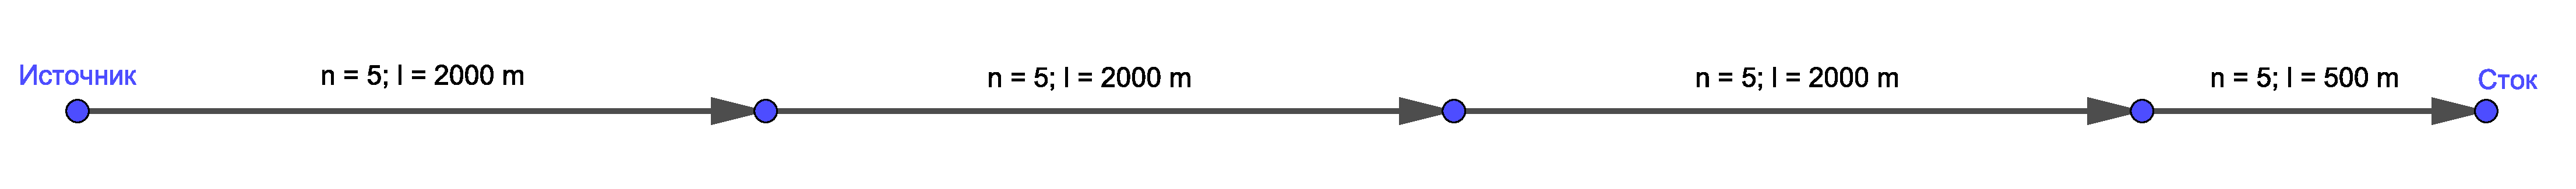
\includegraphics[width=1.0\linewidth]{scheme_simple_3block_road.eps}
       \caption{}
    \end{subfigure}

    \begin{subfigure}[b][][b]{1.0\textwidth}
       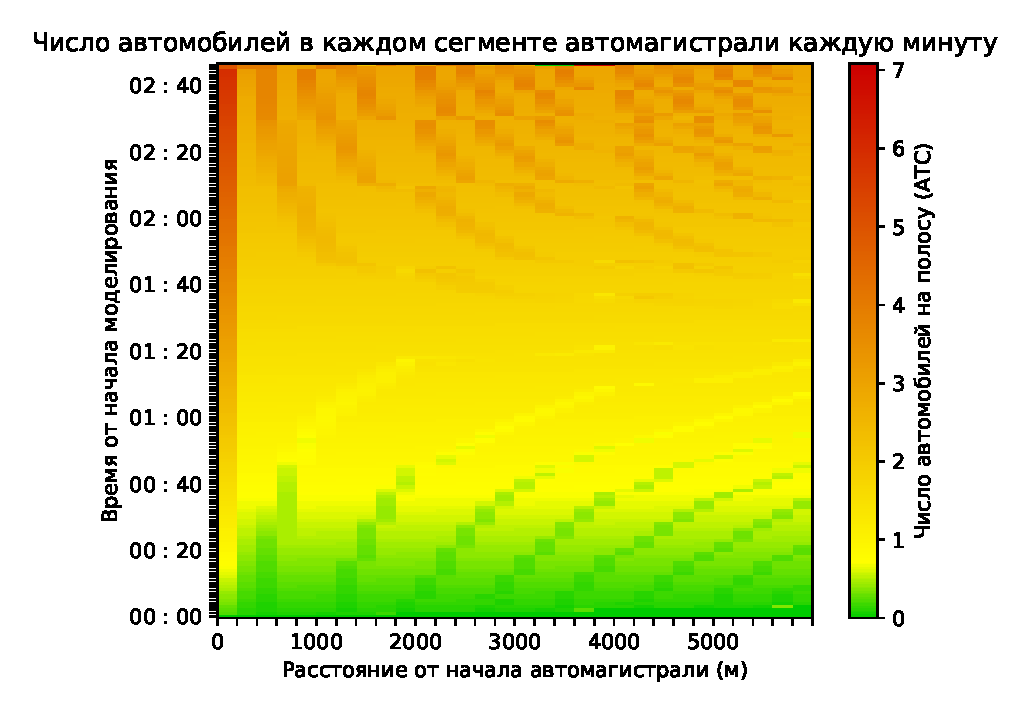
\includegraphics[width=1.0\linewidth]{simple_3_block_road.eps}
       \caption{}
    \end{subfigure}

    \caption{а) Схема простой дороги в модели состоит из 3 сегментов по 2 километра. б) Тепловая карта автомобилей на простой дороге без перекрестков с линейно нарастающим вплоть до 150 АТС/мин потоком.}
    \label{fig:simple_road}
\end{figure}

\subsection{Прямая дорога с сужением и синусоидальным потоком}
Для следующего эксперимента возьмем прямой участок пятиполосной дороги с сужением до двухполосной.
В данном эксперименте с целью рассмотрения как процесса формирования затора, так и его исчезновения пустим на вход синусоидальный поток с периодом равным времени моделирования и амплитудой в 85 АТС/мин.
Результат моделирования можно наблюдать на фиг.~\ref{fig:jammed_5-2_3block_road_sin_wave}.
На графике видно, что при уменьшении потока на сегменте, соответствующем двухполосной дороге, наблюдается разрыв потока АТС, который мы связываем с групповыми эффектами модели.
\begin{figure}[ht]
    \begin{subfigure}[b][][b]{1.0\textwidth}
       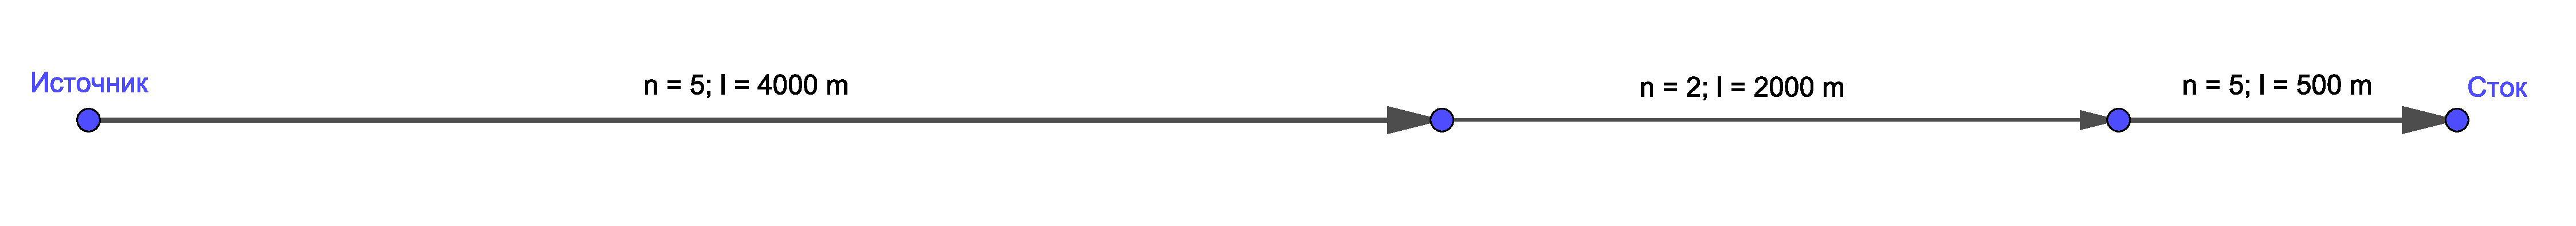
\includegraphics[width=1.0\linewidth]{scheme_jammed_sin_wave.eps}
       \caption{}
    \end{subfigure}

    \begin{subfigure}[b][][b]{1.0\textwidth}
       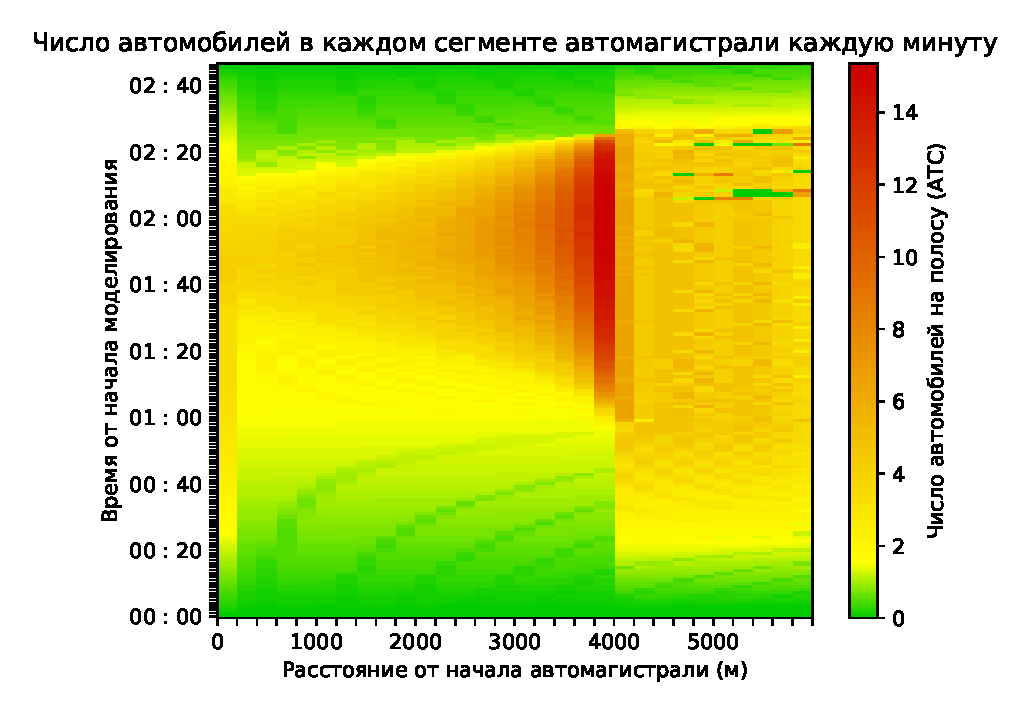
\includegraphics[width=1.0\linewidth]{jammed_5-2_3block_road_sin_wave.eps}
       \caption{}
    \end{subfigure}

    \caption{а) Схема дороги. б) Тепловая карта автомобилей на пятиполосной дороге без перекрестков с сужением до двух полос и синусоидальным потоком на входе.}
    \label{fig:jammed_5-2_3block_road_sin_wave}
\end{figure}

\subsection{Прямая дорога с пропадающим сужением}
Также рассмотрим ситуацию, когда при постоянном потоке в 100 АТС/мин на пятиполосной дороге с сужением до двухполосной данное сужение в середине моделирования пропадает.
Такая ситуация может сложиться, например, при прекращении ремонтных работ или устранении аварии. Результаты моделирования можно наблюдать на фиг.~\ref{fig:jammed_5-2_3block_road_with_unjam}.
\begin{figure}[ht]
    \begin{subfigure}[b]{1.0\textwidth}
       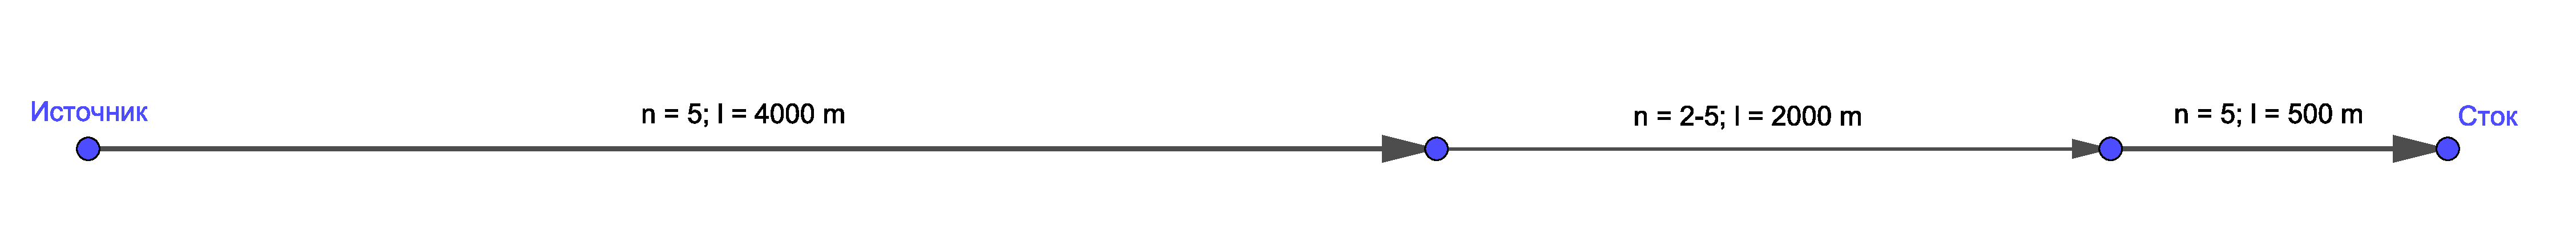
\includegraphics[width=1.0\linewidth]{scheme_jammed_with_unjam.eps}
       \caption{}
    \end{subfigure}

    \begin{subfigure}[b]{1.0\textwidth}
       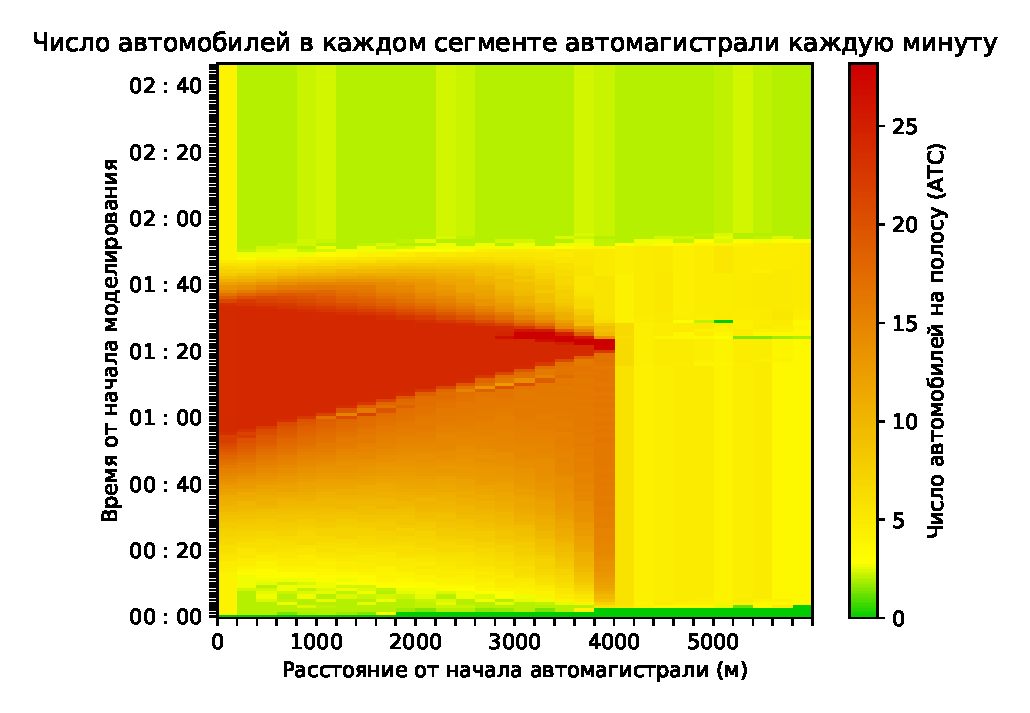
\includegraphics[width=1.0\linewidth]{jammed_5-2_3block_road_with_unjam.eps}
       \caption{}
    \end{subfigure}

    \caption{а) Схема дороги. б) Тепловая карта автомобилей на пятиполосной дороге без перекрестков с сужением до двух полос пропадающим в середине моделирования и постоянным потоком в 100 АТС/мин.}
    \label{fig:jammed_5-2_3block_road_with_unjam}
\end{figure}

\subsection{Перекресток со съездом}
Промоделируем оба варианта перекрестков возможных в предложенной модели.
Перекресток со съездом и перекресток с въездом. В обоих случаях основная автомагистраль -- пятиполосная. Въезд или съезд однополосные.

В эксперименте со съездом входной поток -- 65 АТС/мин. Доля съезжающих автомобилей линейно растет с 20\% до 60\%. На фиг.~\ref{fig:jamming_crossroad_exit_5_1} видно, что из за недостаточной пропускной способности съезда на основной автомагистрали образуется пробка.
\begin{figure}[ht]
    \begin{subfigure}[b]{1.0\textwidth}
       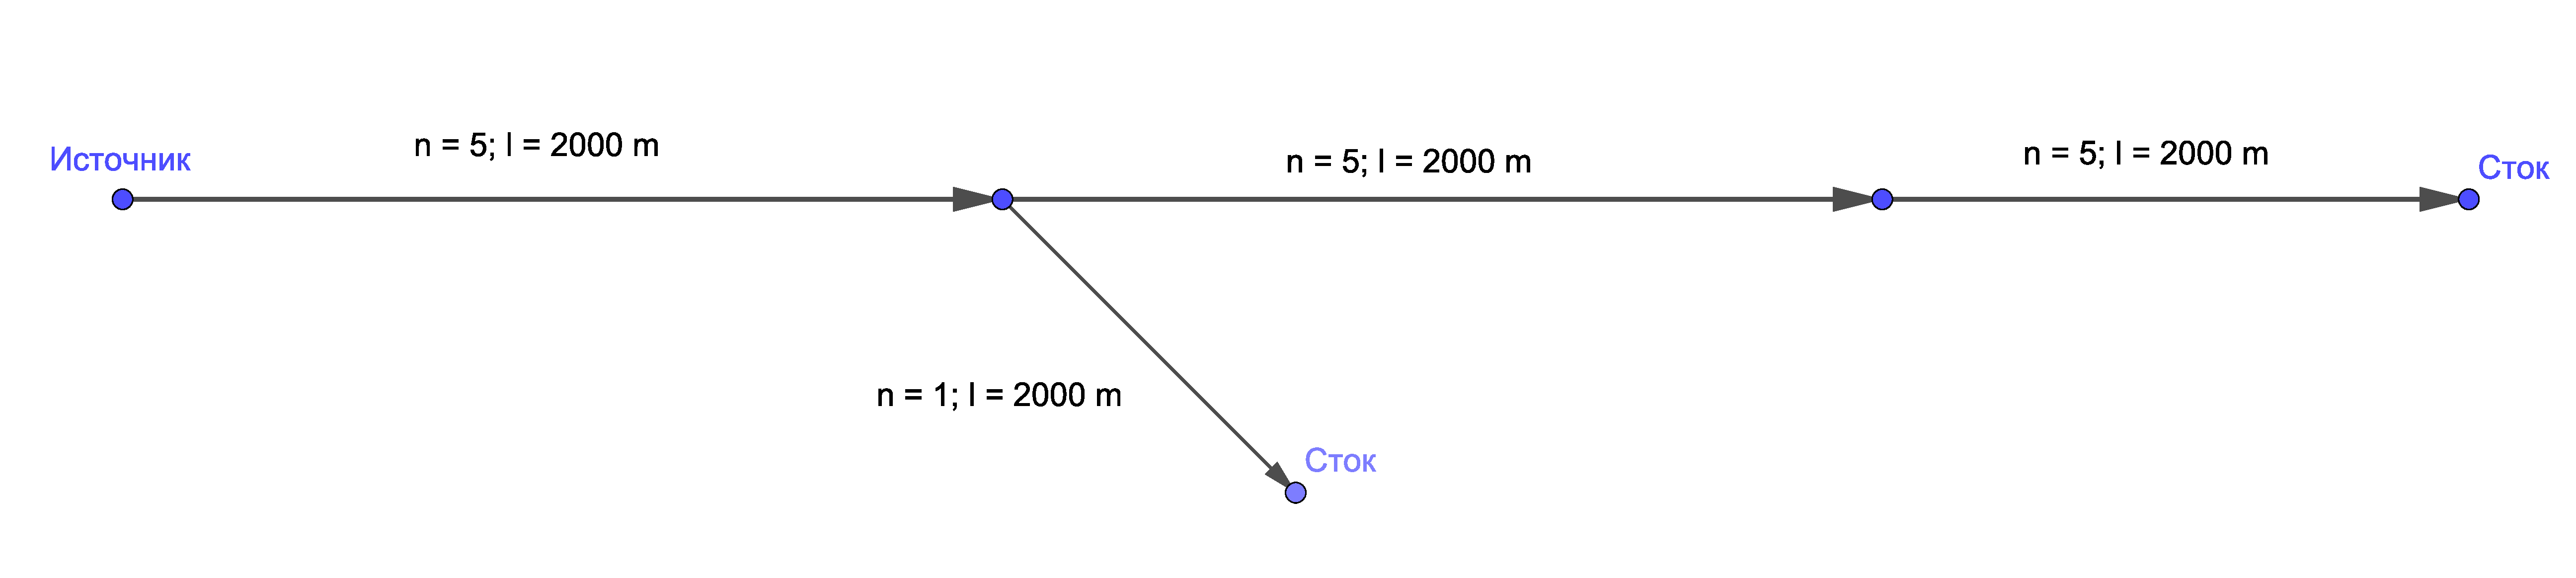
\includegraphics[width=1.0\linewidth]{scheme_jammed_crossroad_exit.eps}
       \caption{}
    \end{subfigure}

    \begin{subfigure}[b]{1.0\textwidth}
       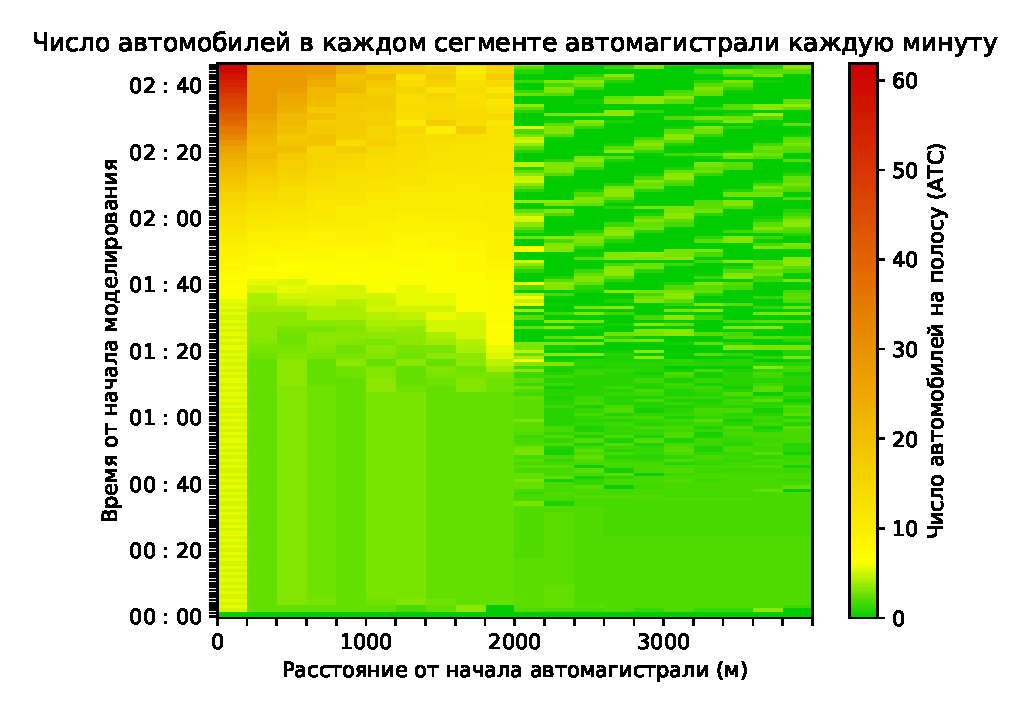
\includegraphics[width=1.0\linewidth]{jamming_crossroad_exit_5_1.eps}
       \caption{}
    \end{subfigure}

    \caption{а) Схема дороги. б) Тепловая карта автомобилей на пятиполосной дороге со съездом.}
    \label{fig:jamming_crossroad_exit_5_1}
\end{figure}

\subsection{Перекресток с въездом}
В эксперименте со въездом поток на автомагистрали~--- 140 АТС/мин, поток на въезде линейно растет от 20 до 50 АТС/мин. В данном случае также образуется пробка на основной автомагистрали, что видно на фиг.~\ref{fig:jamming_crossroad_enter_5_1}.
\begin{figure}[ht]
    \begin{subfigure}[b]{1.0\textwidth}
       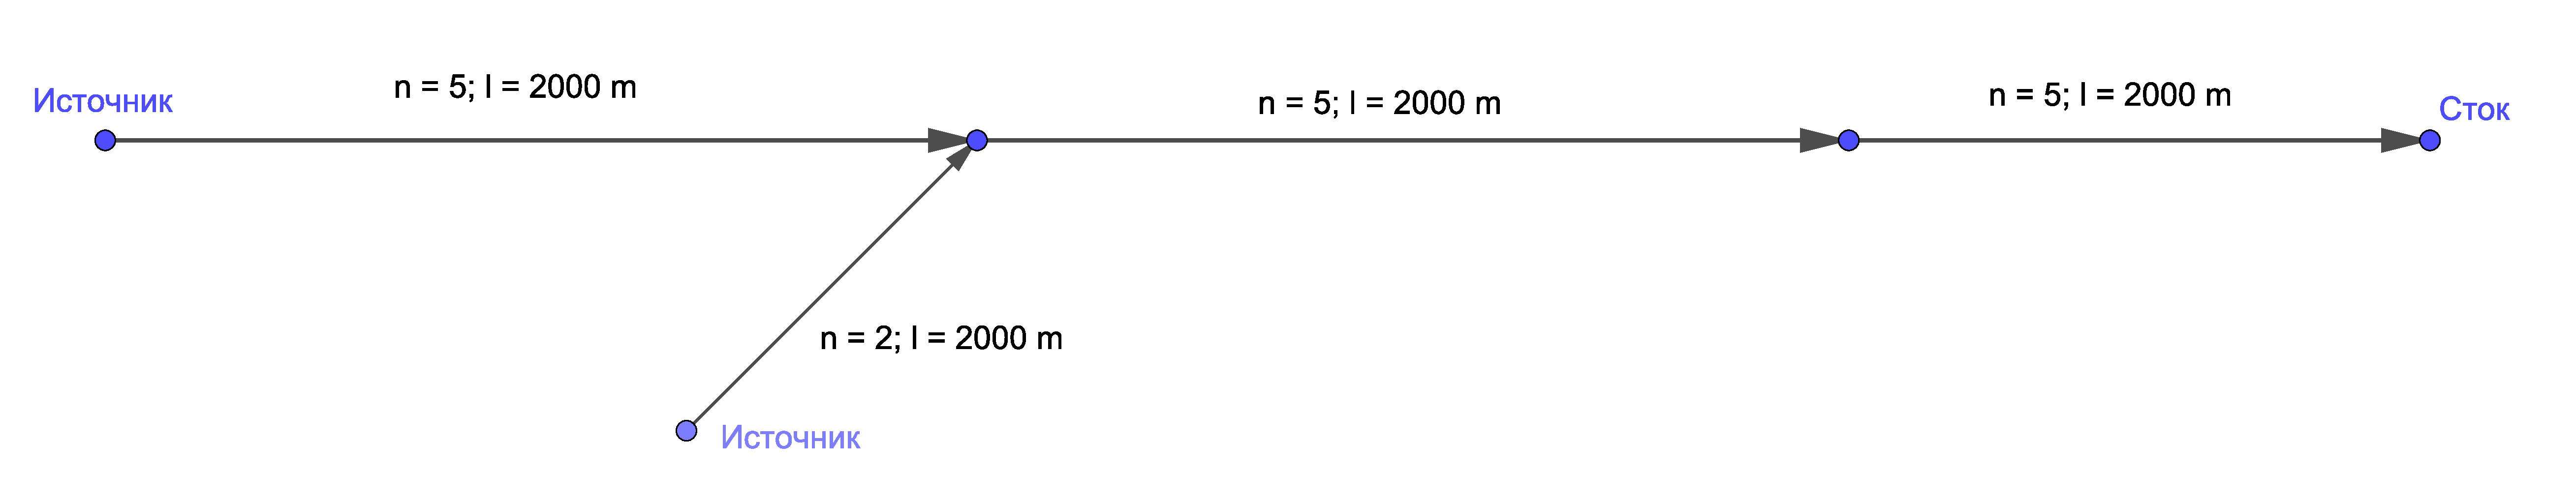
\includegraphics[width=1.0\linewidth]{scheme_jammed_crossroad_enter.eps}
       \caption{}
    \end{subfigure}

    \begin{subfigure}[b]{1.0\textwidth}
       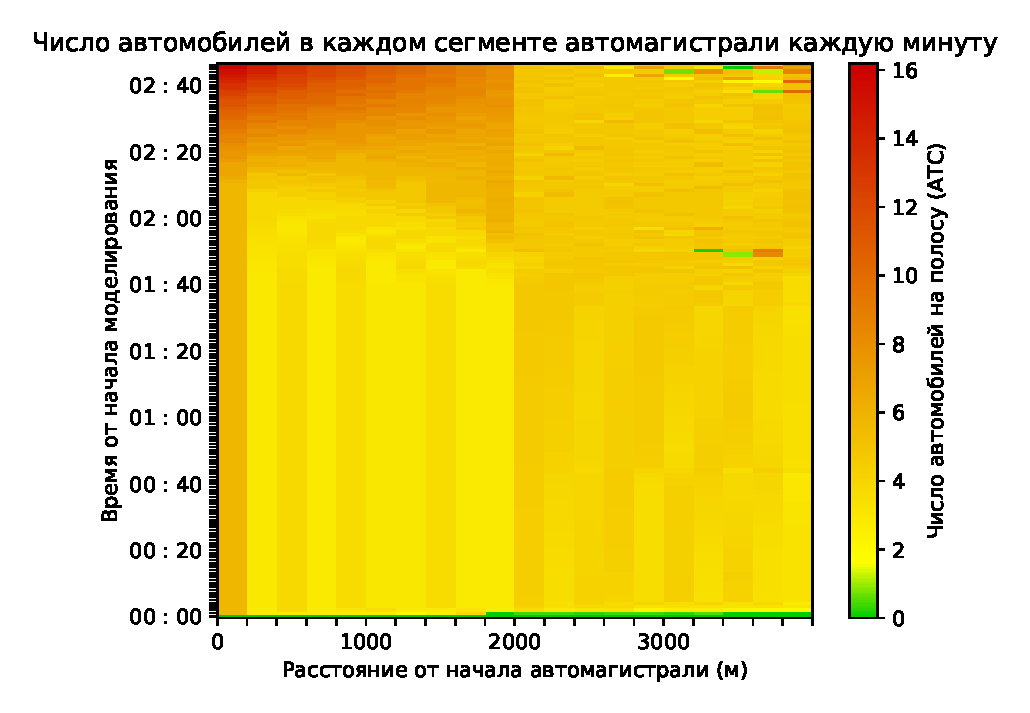
\includegraphics[width=1.0\linewidth]{jamming_crossroad_enter_5_2.eps}
       \caption{}
    \end{subfigure}

    \caption{а) Схема дороги. б) Тепловая карта автомобилей на пятиполосной дороге со въездом с постепенно нарастающем потоком с него.}
    \label{fig:jamming_crossroad_enter_5_1}
\end{figure}

\section{Данные дорожных датчиков}
\subsection{Прямая дорога}
\label{sec::experiment_1}
В данном эксперименте мы воспользовались построенной для данного участка автомагистрали фундаментальной диаграммой~\cite{collectiveArticle2}.
Полный временной интервал эксперимента~--- одна неделя, графики приведены за один день.
В приведенном эксперименте проводится проверка результатов модели в простейшем случае моделирования числа съехавших АТС по числу въехавших на участке автомагистрали без въездов и съездов.
Результаты видны на графике~\ref{fig:MCAR_simple_test}.
\begin{figure}[ht]
    \centerfloat{
        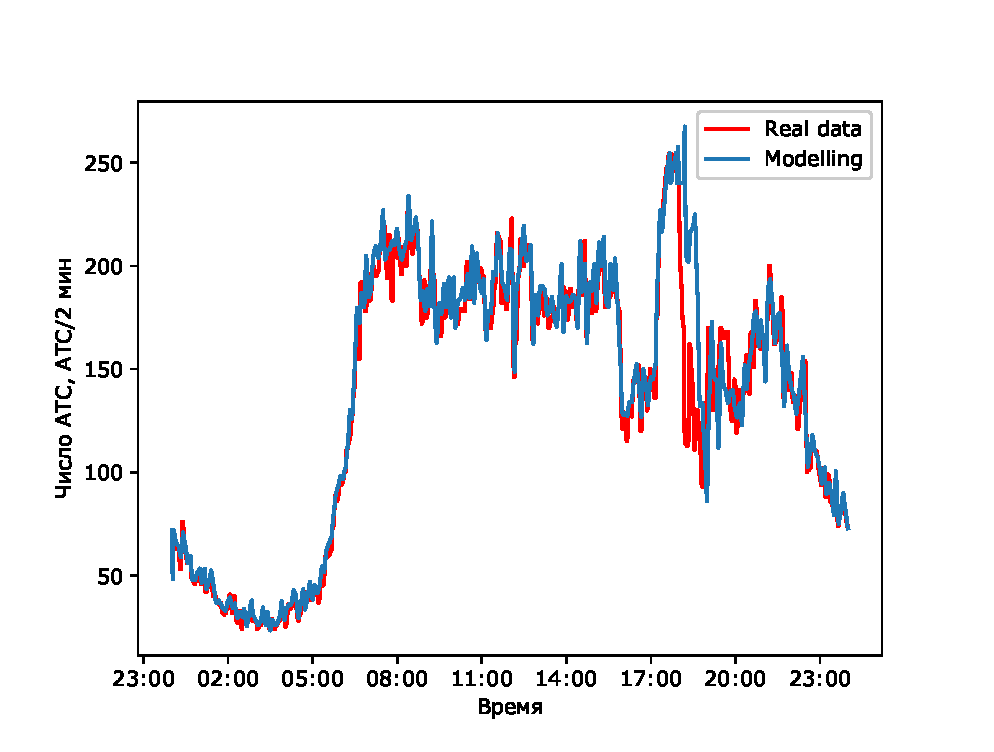
\includegraphics[width=1.0\linewidth]{MCAR_simple_test.eps}
    }
    \caption{График полученного с помощью модели числа съехавших АТС (красная линия) в сравнении с числом съехавших АТС зафиксированных дорожным датчиком (синяя линия) за один день. Среднеквадратичная ошибка $S = 18.4$.}
    \label{fig:MCAR_simple_test}
\end{figure}
Среднеквадратичная ошибка $S = 18.4$.

\subsection{Эксперимент с перекрытием полосы}
\label{sec::experiment_2}
Во втором эксперименте на основе реальных данных проводится моделирование ситуации, когда одна из полос на автомагистрали перекрывается.
Сам эксперимент проводится на том же участке автомагистрали и за тот же промежуток времени, что и первый в разделе~\ref{sec::experiment_1}.
В данном эксперименте у нас нет данных для расчета среднеквадратичной ошибки и он был поставлен для рассмотрения поведения модели в данной ситуации.
Результаты за тот же день, что и в первом эксперименте на данных дорожных датчиков можно увидеть на графике~\ref{fig:MCAR_minus_road_test}.
\begin{figure}[ht]
    \centerfloat{
        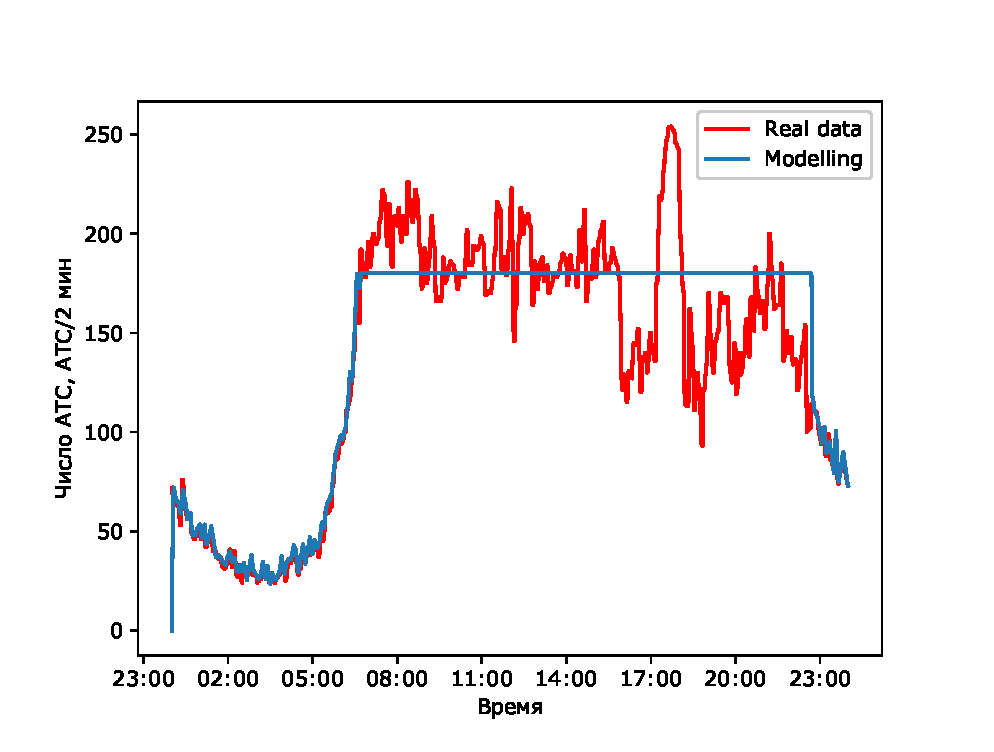
\includegraphics[width=1.0\linewidth]{MCAR_minus_line.eps}
    }
    \caption{График полученного с помощью модели числа съехавших АТС (красная линия) в сравнении с числом съехавших АТС зафиксированных дорожным датчиком (синяя линия) за один день.}
    \label{fig:MCAR_minus_road_test}
\end{figure}

Видно, что АТС не могут съехать из за того, что пропускная способность автомагистрали снизилась, что приводит к появлению горизонтальной линии на графике.
Однако, через некоторое время после того как поток должен был спасть, что видно на графике реальных данных за тот же временной промежуток, дорога освобождается и результат моделирования приходит в соответствие с реальными данными.

\section{Обсуждение результатов раздела}
Эксперименты из данной главы показывают работоспособность модели для моделирования всевозможных конфигураций автомагистрали при любом потоке АТС на ней.
Показано, что модель адекватно симулирует поведение АТС на автомагистрали как в ситуации достаточной ее пропускной способности, так и при ее превышении, а также моделирует различные варианты образования заторных ситуации как при распространении пробки из за проблем на магистрали на фиг.~\ref{fig:jammed_5-2_3block_road_sin_wave}, так и по причине недостаточной пропускной способности прилегающих съездов~\ref{fig:jamming_crossroad_exit_5_1}.

Также на реальных данных видно~\ref{fig:MCAR_simple_test}, что в модели нет потери автомобилей и она моделирует реальный участок автомагистрали в соответствии с зафиксированными дорожными датчиками данными.
Тут надо также понимать, что полученная небольшая ошибка связана как с несовершенством модели, так и с ошибками в видеофиксации дорожными датчиками.

Эксперимент изображенный на~\ref{fig:MCAR_minus_road_test} показывает состоятельность модели при перекрытии части автомагистрали~--- видно, что при уменьшении потока АТС пробка исчезает и результаты приходят в соответствие с реальными данными.

\FloatBarrier            % Глава 4
\chapter{Вычислительные эксперименты. Проверка работоспособности модели}\label{ch:ch4}

В первую очередь необходимо проверить адекватность вышеизложенного подхода на модельных данных во всех режимах работы автомагистрали.
В данном разделе проводится два типа экспериментов~--- на модельных и на реальных данных, оба призваны проверить поведение модели в различных конфигурациях дорожной сети.

Эксперименты на модельных данных сводятся к проверке поведение модели на соответствие реально наблюдаемым процессам на простейших сегментах транспортной сети~--- прямой дороге, стыке двух дорог, съезд с автомагистрали, въезд на автомагистраль.
Графики представляют из себя тепловые карты по оси $x$ которой отложено расстояние от начала участка магистрали, по оси $y$~-- время.
В конце автомагистрали всегда находится небольшая ветвь представляющий из себя сток.

Эксперименты на реальных данных проводятся для участка МКАД между 99 и 101 километром с помощью расположенных на этом участке автомагистрали дорожных датчиков.
Один из датчиков используется для генерации автомобилей на въезде в моделируемый участок магистрали, второй~--- для верификации результатов.
Проводятся два эксперимента~--- эксперимент с моделированием прямой дороги и эксперимент с виртуальным перекрытием одной из полос магистрали.
В первом эксперименте рассчитывается показатель среднеквадратической ошибки
\[
    S = \sqrt{\frac{1}{K}\sum_{k=1}^K (n(k) - \bar{n}(k)},
\]
где $K$~--- число временных интервалов, $\bar{n}$~--- зафиксированное дорожным датчиком число проехавших по участку магистрали АТС с целью верификации результатов моделирования на реальных данных.

\section{Модельные данные}
\subsection{Прямая дорога}
Для начала рассмотрим поведение модели для простой пятиполосной дороги длиной 6 километров без перекрестков с линейно нарастающим вплоть до 150 АТС/мин потоком изображенное на фиг.~\ref{fig:simple_road}. В модели данная дорога представлена тремя ветвями по 2 километра.
Данный эксперимент показывает, что в модели нет существенных краевых эффектов на стыке ветвей.
\begin{figure}[ht]
    \begin{subfigure}[b][][b]{1.0\textwidth}
       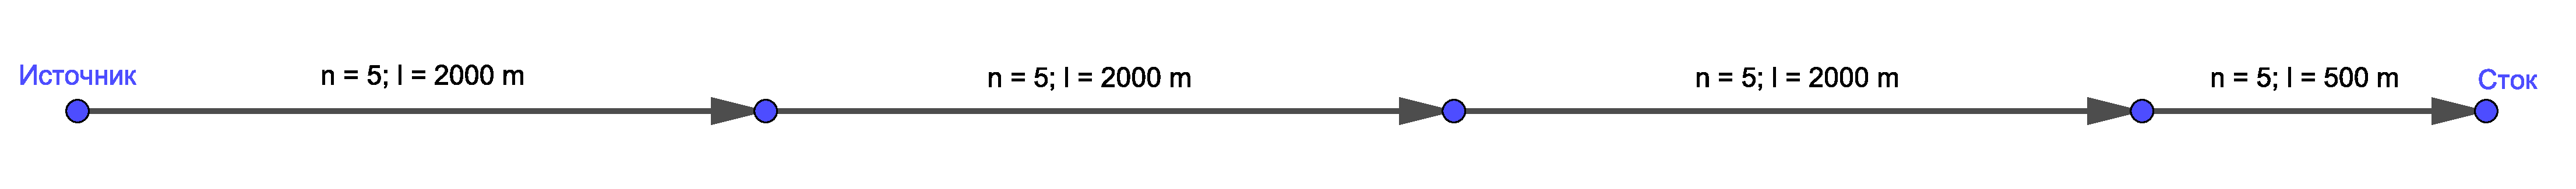
\includegraphics[width=1.0\linewidth]{scheme_simple_3block_road.eps}
       \caption{}
    \end{subfigure}

    \begin{subfigure}[b][][b]{1.0\textwidth}
       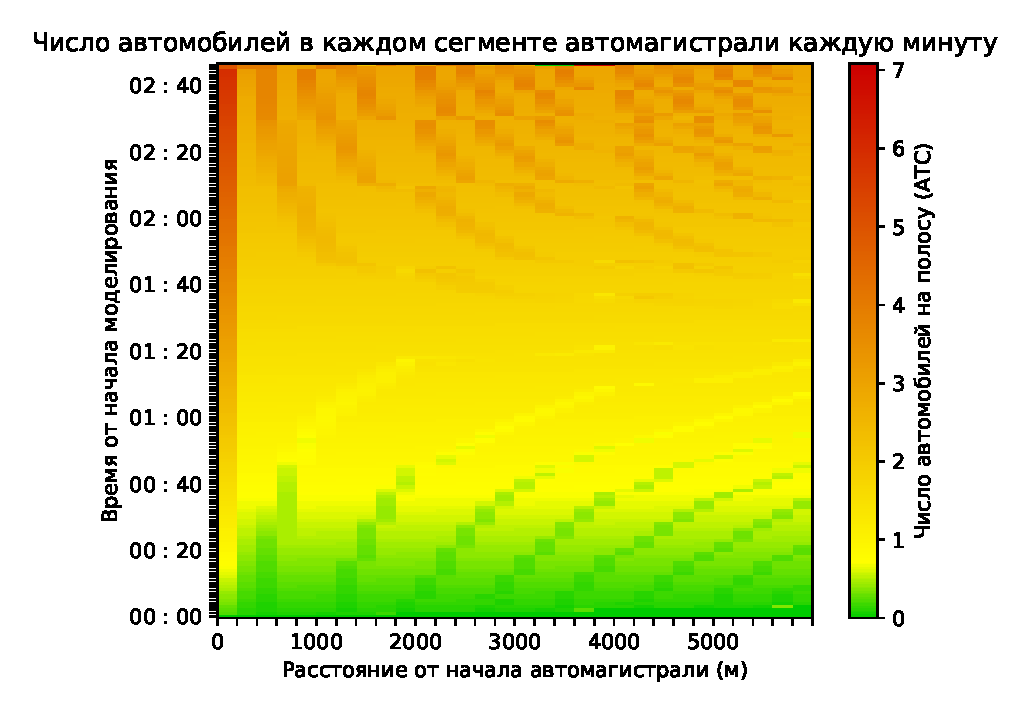
\includegraphics[width=1.0\linewidth]{simple_3_block_road.eps}
       \caption{}
    \end{subfigure}

    \caption{а) Схема простой дороги в модели состоит из 3 сегментов по 2 километра. б) Тепловая карта автомобилей на простой дороге без перекрестков с линейно нарастающим вплоть до 150 АТС/мин потоком.}
    \label{fig:simple_road}
\end{figure}

\subsection{Прямая дорога с сужением и синусоидальным потоком}
Для следующего эксперимента возьмем прямой участок пятиполосной дороги с сужением до двухполосной.
В данном эксперименте с целью рассмотрения как процесса формирования затора, так и его исчезновения пустим на вход синусоидальный поток с периодом равным времени моделирования и амплитудой в 85 АТС/мин.
Результат моделирования можно наблюдать на фиг.~\ref{fig:jammed_5-2_3block_road_sin_wave}.
На графике видно, что при уменьшении потока на сегменте, соответствующем двухполосной дороге, наблюдается разрыв потока АТС, который мы связываем с групповыми эффектами модели.
\begin{figure}[ht]
    \begin{subfigure}[b][][b]{1.0\textwidth}
       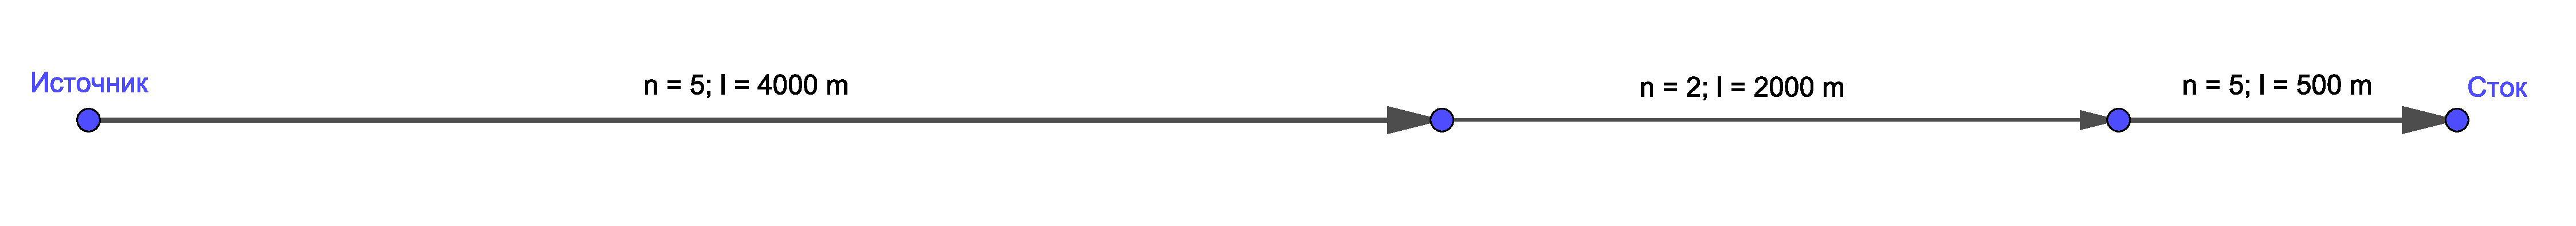
\includegraphics[width=1.0\linewidth]{scheme_jammed_sin_wave.eps}
       \caption{}
    \end{subfigure}

    \begin{subfigure}[b][][b]{1.0\textwidth}
       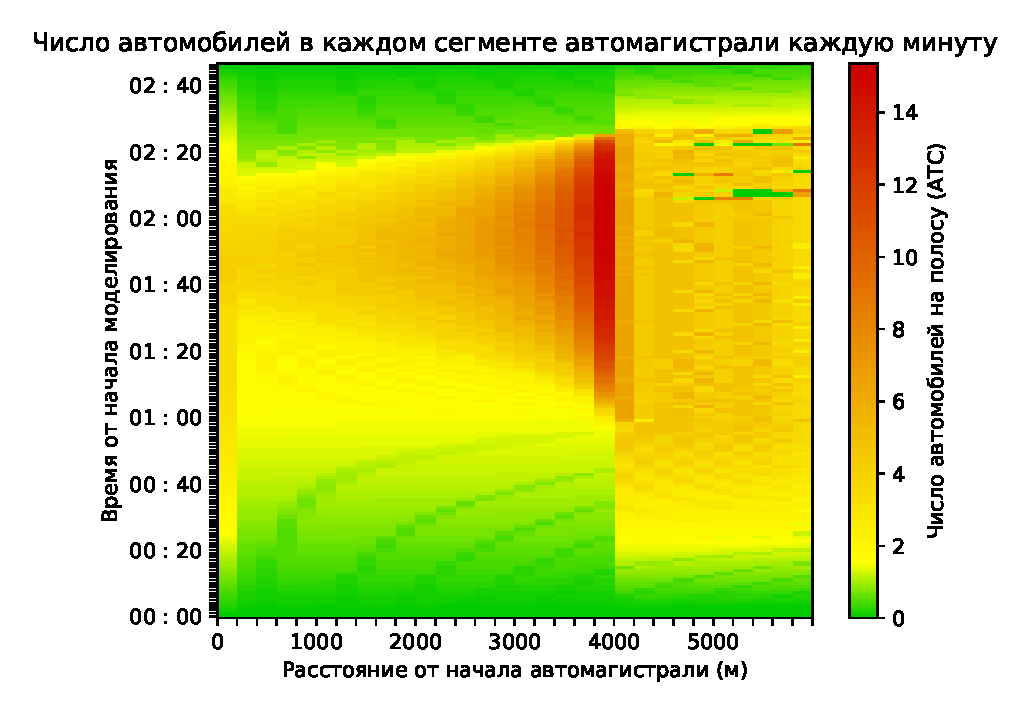
\includegraphics[width=1.0\linewidth]{jammed_5-2_3block_road_sin_wave.eps}
       \caption{}
    \end{subfigure}

    \caption{а) Схема дороги. б) Тепловая карта автомобилей на пятиполосной дороге без перекрестков с сужением до двух полос и синусоидальным потоком на входе.}
    \label{fig:jammed_5-2_3block_road_sin_wave}
\end{figure}

\subsection{Прямая дорога с пропадающим сужением}
Также рассмотрим ситуацию, когда при постоянном потоке в 100 АТС/мин на пятиполосной дороге с сужением до двухполосной данное сужение в середине моделирования пропадает.
Такая ситуация может сложиться, например, при прекращении ремонтных работ или устранении аварии. Результаты моделирования можно наблюдать на фиг.~\ref{fig:jammed_5-2_3block_road_with_unjam}.
\begin{figure}[ht]
    \begin{subfigure}[b]{1.0\textwidth}
       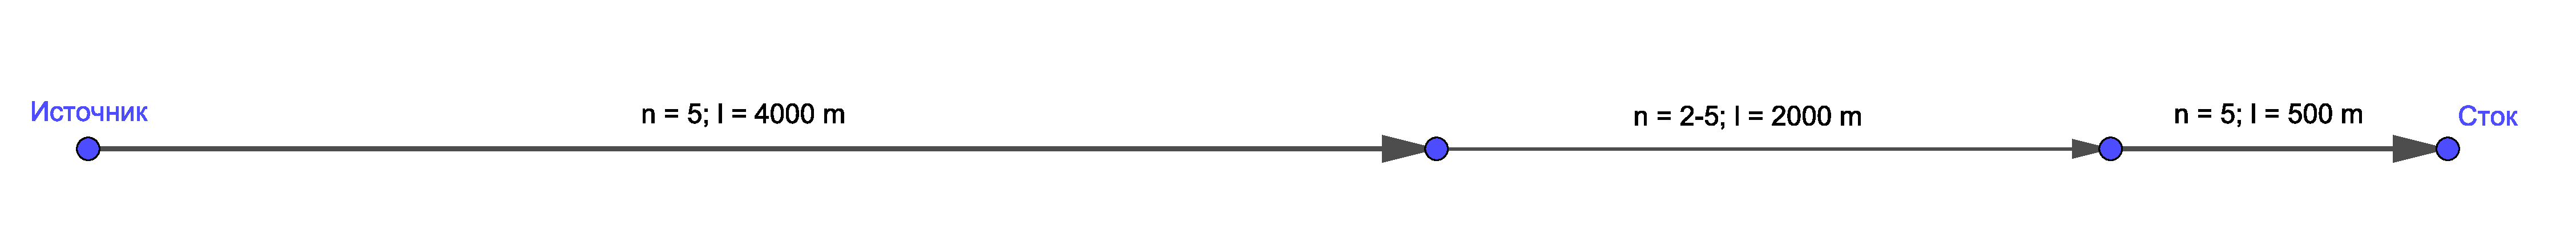
\includegraphics[width=1.0\linewidth]{scheme_jammed_with_unjam.eps}
       \caption{}
    \end{subfigure}

    \begin{subfigure}[b]{1.0\textwidth}
       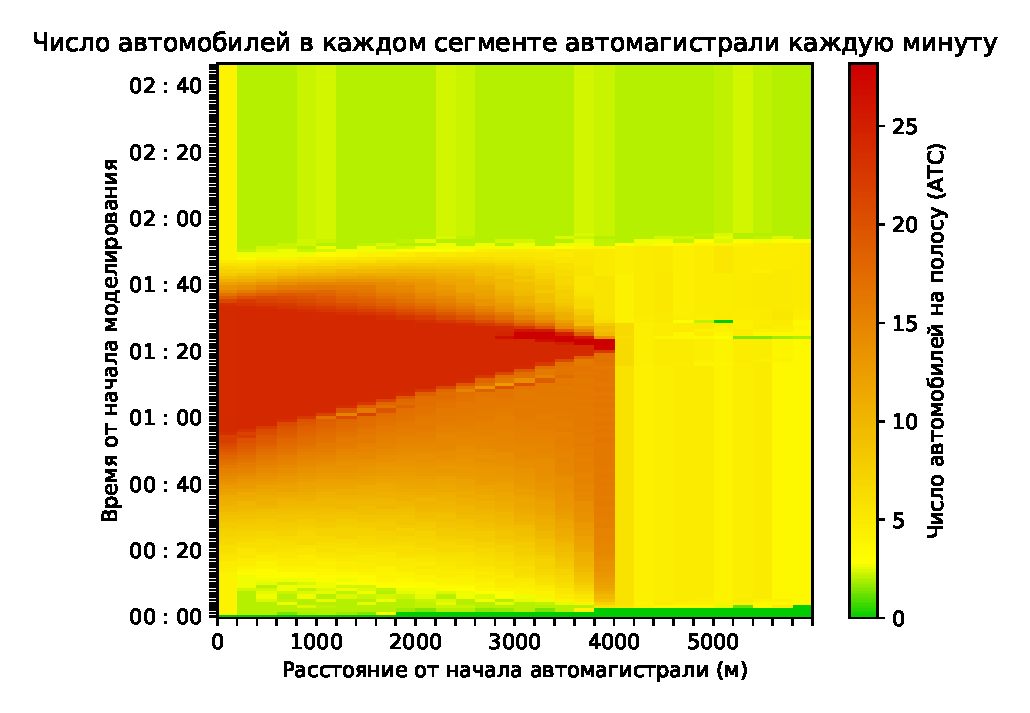
\includegraphics[width=1.0\linewidth]{jammed_5-2_3block_road_with_unjam.eps}
       \caption{}
    \end{subfigure}

    \caption{а) Схема дороги. б) Тепловая карта автомобилей на пятиполосной дороге без перекрестков с сужением до двух полос пропадающим в середине моделирования и постоянным потоком в 100 АТС/мин.}
    \label{fig:jammed_5-2_3block_road_with_unjam}
\end{figure}

\subsection{Перекресток со съездом}
Промоделируем оба варианта перекрестков возможных в предложенной модели.
Перекресток со съездом и перекресток с въездом. В обоих случаях основная автомагистраль -- пятиполосная. Въезд или съезд однополосные.

В эксперименте со съездом входной поток -- 65 АТС/мин. Доля съезжающих автомобилей линейно растет с 20\% до 60\%. На фиг.~\ref{fig:jamming_crossroad_exit_5_1} видно, что из за недостаточной пропускной способности съезда на основной автомагистрали образуется пробка.
\begin{figure}[ht]
    \begin{subfigure}[b]{1.0\textwidth}
       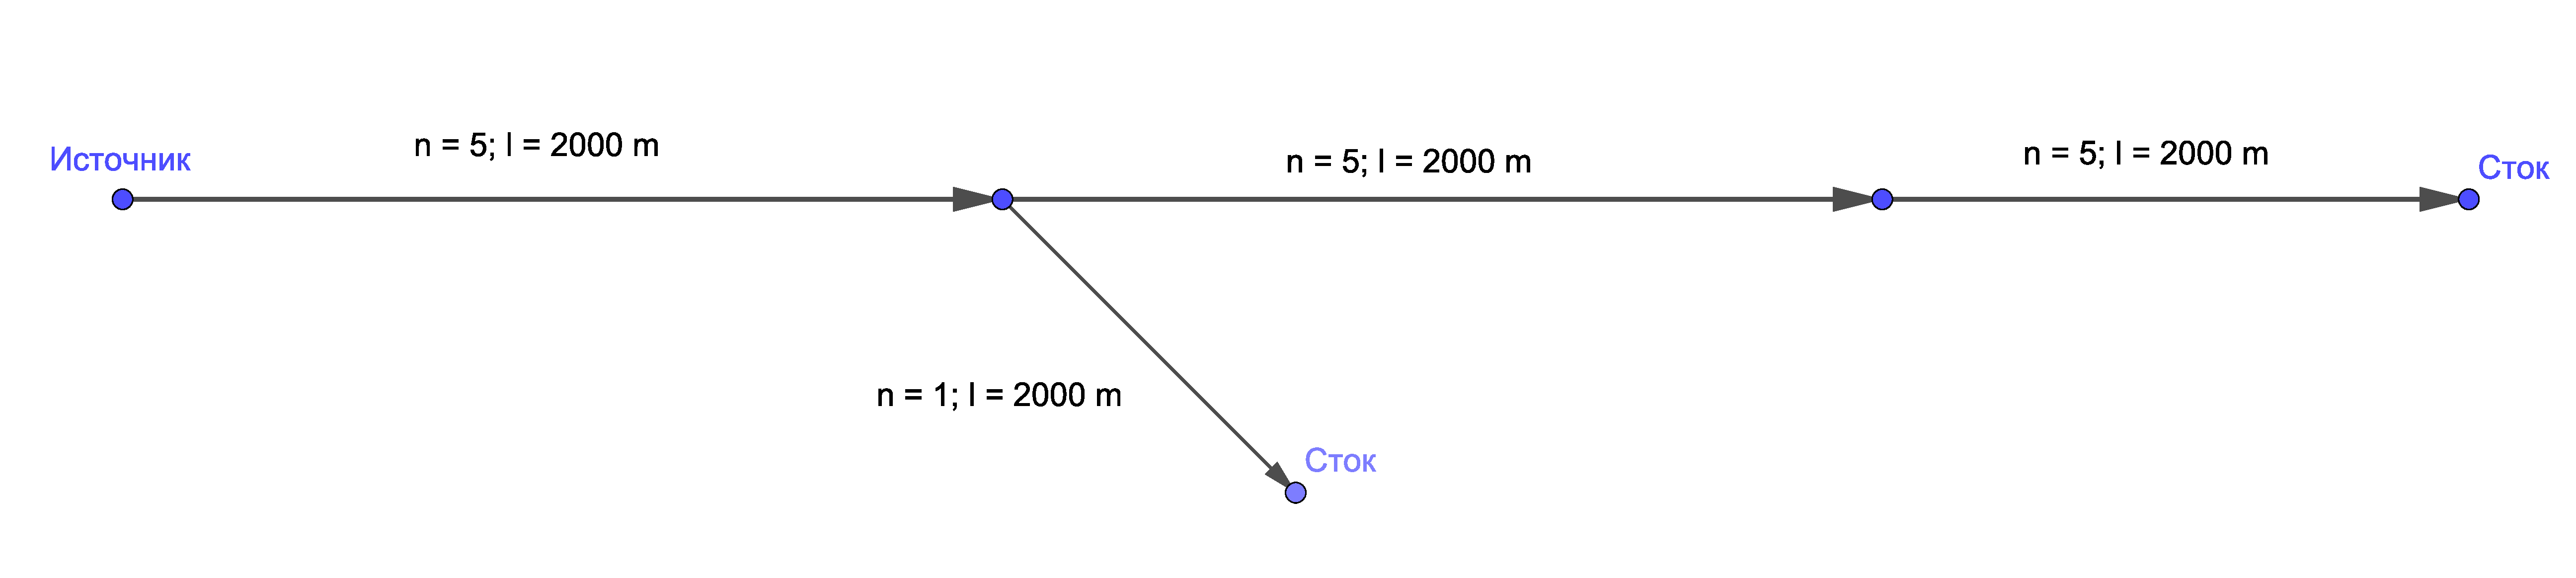
\includegraphics[width=1.0\linewidth]{scheme_jammed_crossroad_exit.eps}
       \caption{}
    \end{subfigure}

    \begin{subfigure}[b]{1.0\textwidth}
       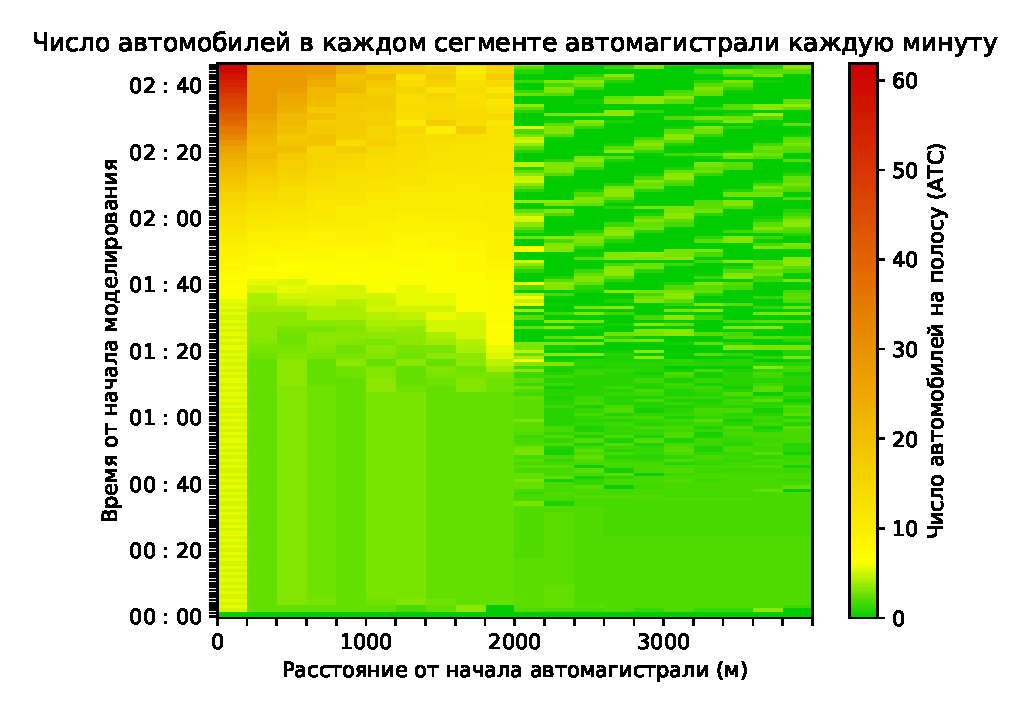
\includegraphics[width=1.0\linewidth]{jamming_crossroad_exit_5_1.eps}
       \caption{}
    \end{subfigure}

    \caption{а) Схема дороги. б) Тепловая карта автомобилей на пятиполосной дороге со съездом.}
    \label{fig:jamming_crossroad_exit_5_1}
\end{figure}

\subsection{Перекресток с въездом}
В эксперименте со въездом поток на автомагистрали~--- 140 АТС/мин, поток на въезде линейно растет от 20 до 50 АТС/мин. В данном случае также образуется пробка на основной автомагистрали, что видно на фиг.~\ref{fig:jamming_crossroad_enter_5_1}.
\begin{figure}[ht]
    \begin{subfigure}[b]{1.0\textwidth}
       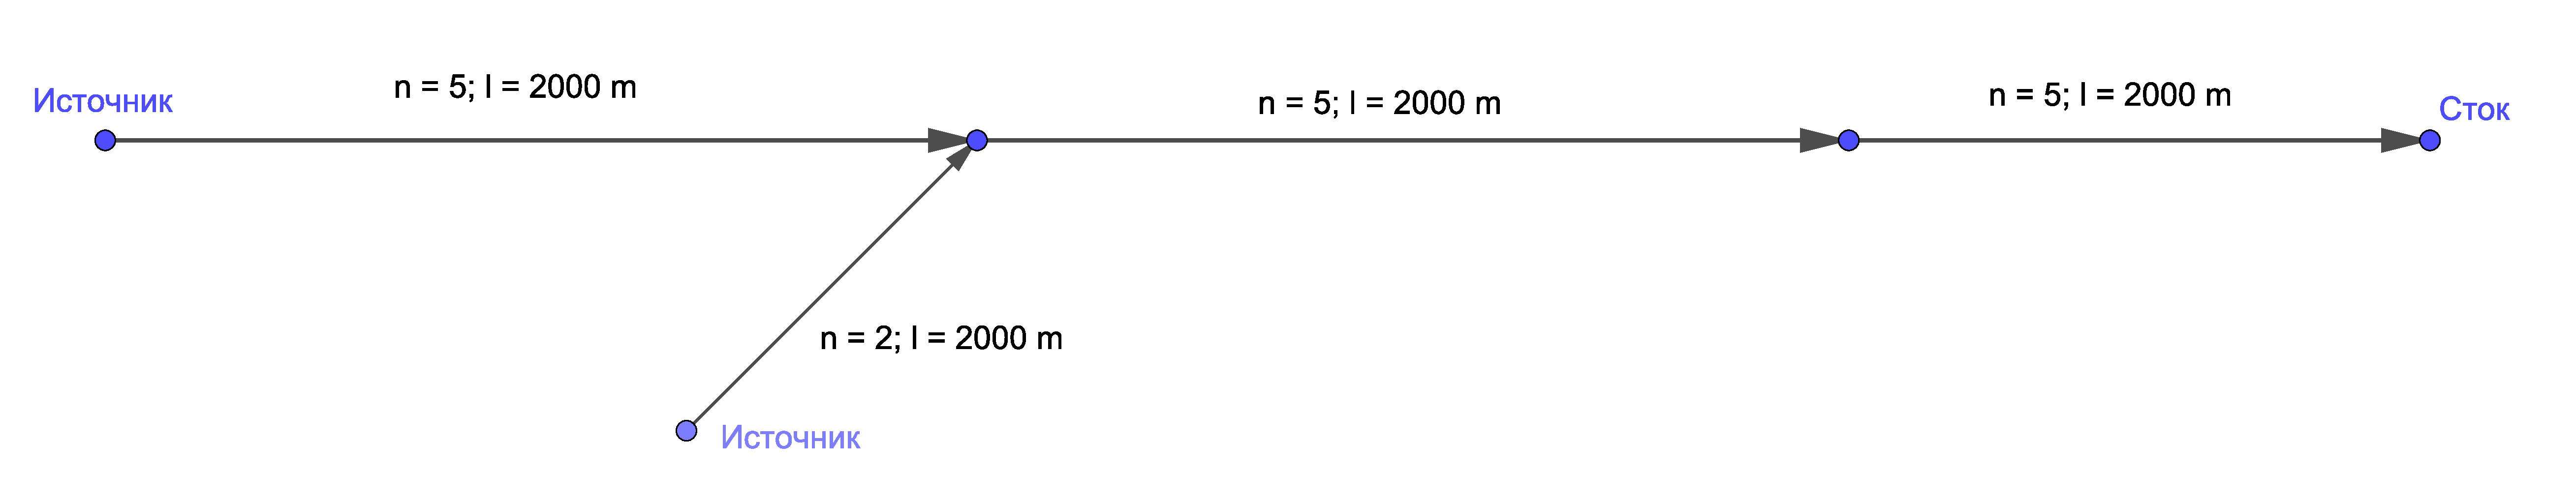
\includegraphics[width=1.0\linewidth]{scheme_jammed_crossroad_enter.eps}
       \caption{}
    \end{subfigure}

    \begin{subfigure}[b]{1.0\textwidth}
       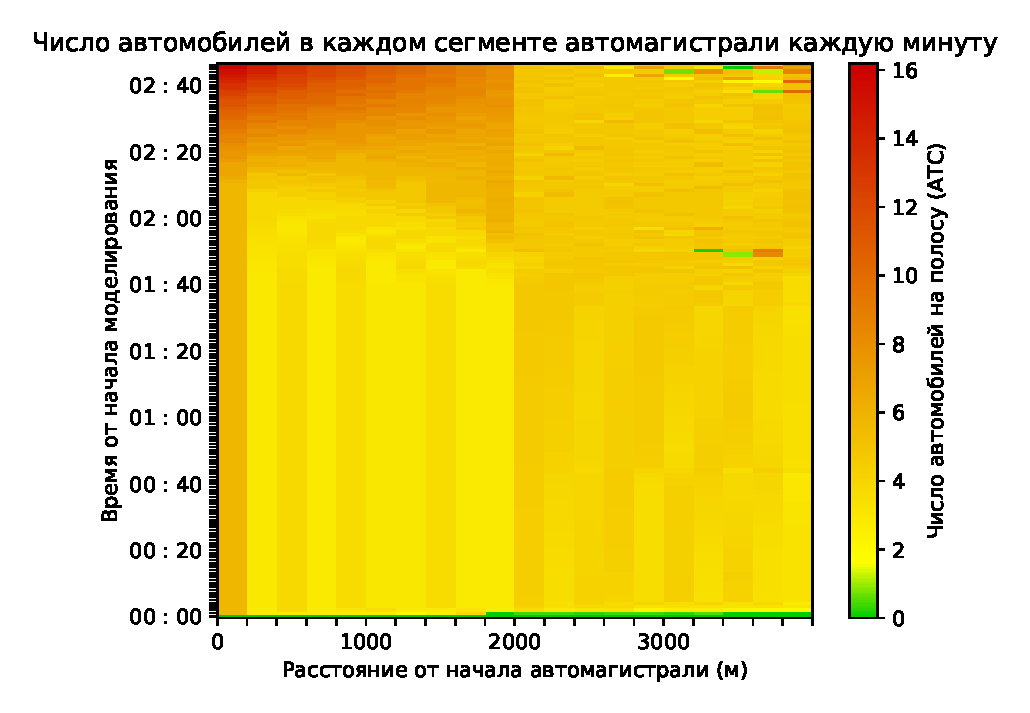
\includegraphics[width=1.0\linewidth]{jamming_crossroad_enter_5_2.eps}
       \caption{}
    \end{subfigure}

    \caption{а) Схема дороги. б) Тепловая карта автомобилей на пятиполосной дороге со въездом с постепенно нарастающем потоком с него.}
    \label{fig:jamming_crossroad_enter_5_1}
\end{figure}

\section{Данные дорожных датчиков}
\subsection{Прямая дорога}
\label{sec::experiment_1}
В данном эксперименте мы воспользовались построенной для данного участка автомагистрали фундаментальной диаграммой~\cite{collectiveArticle2}.
Полный временной интервал эксперимента~--- одна неделя, графики приведены за один день.
В приведенном эксперименте проводится проверка результатов модели в простейшем случае моделирования числа съехавших АТС по числу въехавших на участке автомагистрали без въездов и съездов.
Результаты видны на графике~\ref{fig:MCAR_simple_test}.
\begin{figure}[ht]
    \centerfloat{
        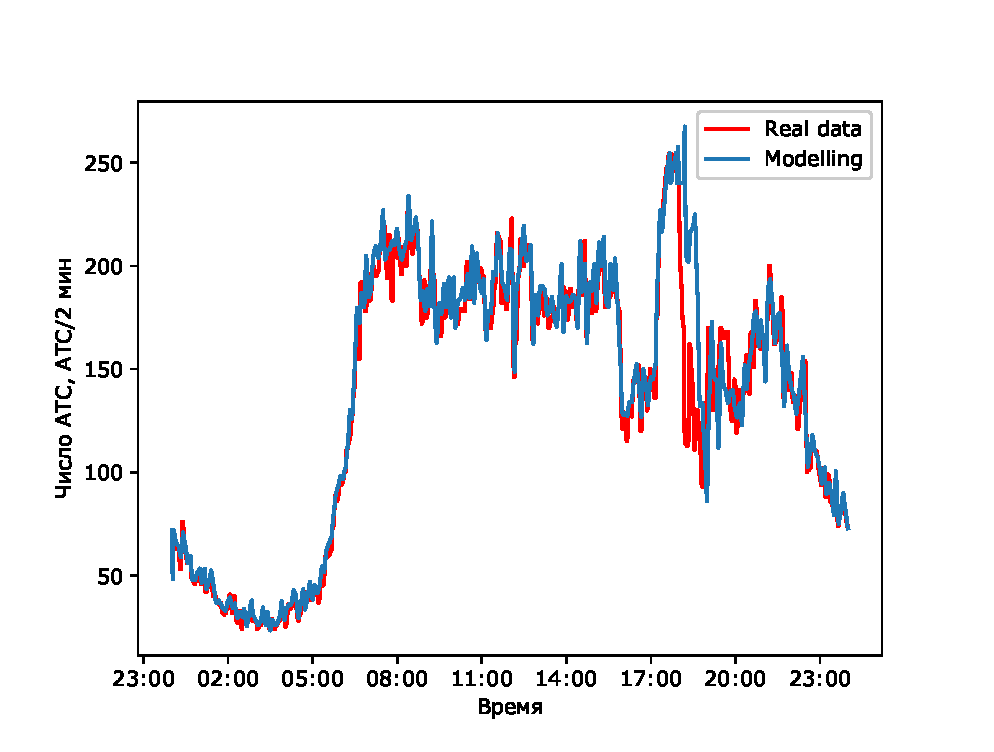
\includegraphics[width=1.0\linewidth]{MCAR_simple_test.eps}
    }
    \caption{График полученного с помощью модели числа съехавших АТС (красная линия) в сравнении с числом съехавших АТС зафиксированных дорожным датчиком (синяя линия) за один день. Среднеквадратичная ошибка $S = 18.4$.}
    \label{fig:MCAR_simple_test}
\end{figure}
Среднеквадратичная ошибка $S = 18.4$.

\subsection{Эксперимент с перекрытием полосы}
\label{sec::experiment_2}
Во втором эксперименте на основе реальных данных проводится моделирование ситуации, когда одна из полос на автомагистрали перекрывается.
Сам эксперимент проводится на том же участке автомагистрали и за тот же промежуток времени, что и первый в разделе~\ref{sec::experiment_1}.
В данном эксперименте у нас нет данных для расчета среднеквадратичной ошибки и он был поставлен для рассмотрения поведения модели в данной ситуации.
Результаты за тот же день, что и в первом эксперименте на данных дорожных датчиков можно увидеть на графике~\ref{fig:MCAR_minus_road_test}.
\begin{figure}[ht]
    \centerfloat{
        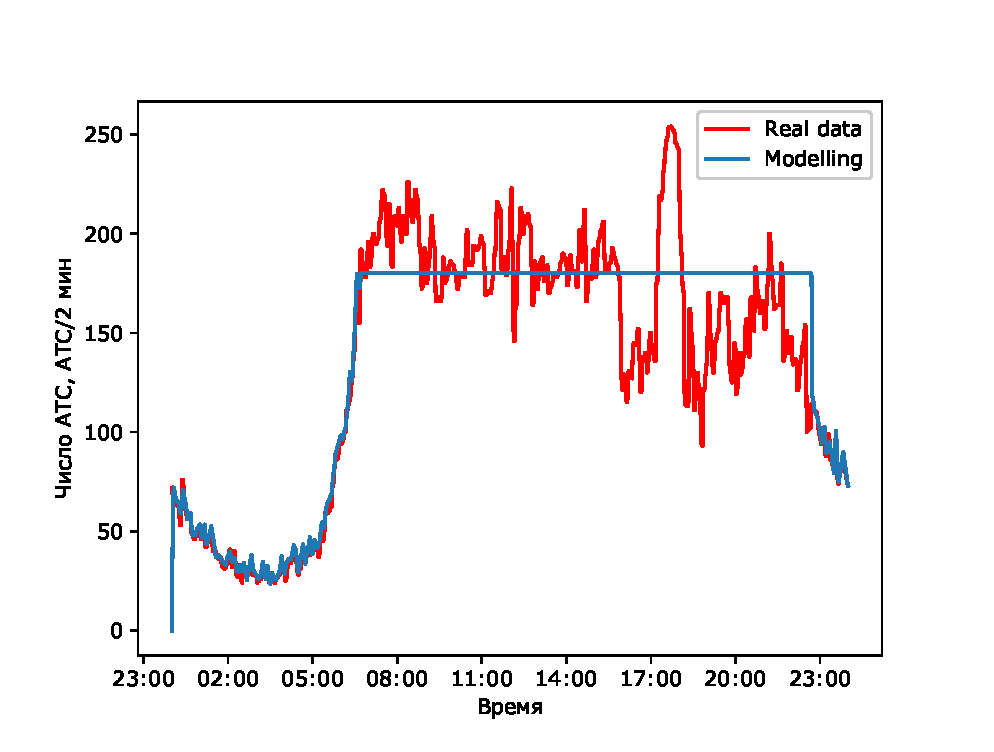
\includegraphics[width=1.0\linewidth]{MCAR_minus_line.eps}
    }
    \caption{График полученного с помощью модели числа съехавших АТС (красная линия) в сравнении с числом съехавших АТС зафиксированных дорожным датчиком (синяя линия) за один день.}
    \label{fig:MCAR_minus_road_test}
\end{figure}

Видно, что АТС не могут съехать из за того, что пропускная способность автомагистрали снизилась, что приводит к появлению горизонтальной линии на графике.
Однако, через некоторое время после того как поток должен был спасть, что видно на графике реальных данных за тот же временной промежуток, дорога освобождается и результат моделирования приходит в соответствие с реальными данными.

\section{Обсуждение результатов раздела}
Эксперименты из данной главы показывают работоспособность модели для моделирования всевозможных конфигураций автомагистрали при любом потоке АТС на ней.
Показано, что модель адекватно симулирует поведение АТС на автомагистрали как в ситуации достаточной ее пропускной способности, так и при ее превышении, а также моделирует различные варианты образования заторных ситуации как при распространении пробки из за проблем на магистрали на фиг.~\ref{fig:jammed_5-2_3block_road_sin_wave}, так и по причине недостаточной пропускной способности прилегающих съездов~\ref{fig:jamming_crossroad_exit_5_1}.

Также на реальных данных видно~\ref{fig:MCAR_simple_test}, что в модели нет потери автомобилей и она моделирует реальный участок автомагистрали в соответствии с зафиксированными дорожными датчиками данными.
Тут надо также понимать, что полученная небольшая ошибка связана как с несовершенством модели, так и с ошибками в видеофиксации дорожными датчиками.

Эксперимент изображенный на~\ref{fig:MCAR_minus_road_test} показывает состоятельность модели при перекрытии части автомагистрали~--- видно, что при уменьшении потока АТС пробка исчезает и результаты приходят в соответствие с реальными данными.

\FloatBarrier            % Глава 5
\chapter{Моделирование МКАД}\label{sec:ch5}
В данном разделе на модельных данных проверим гипотезу о возможности повышения пропускной способности автомагистрали за счет адаптивного управления её въездами на примере МКАД.
Для проверки данной гипотезы на реальных данных у нас недостаточно информации с дорожных датчиков на въезде на МКАД.
В разделе также приводится процедура построения математической модели МКАД с помощью данных топологии GPS-навигатора, обоснование построение модельного потока на въезде и принцип принятия решения автомобилистами о съезде с автомагистрали.

\section{Построение модели МКАД}
\label{sec:MCAR_model}
Модель транспортной сети в данной работе представляет из себя связанный ориентированный граф \(\mathbf{G}\).
Данный граф строится на основе топологии МКАД и прилегающих к нему дорог.
При построении графа вручную размечаются основные ребра-въезды на автомагистраль и ребра-съезды с автомагистрали.
Причем разметка въездов разделяет их на два типа~--- въезды с магистралей, направленных в Москву, и с магистралей, направленных из Москвы.
Это нужно ввиду того, что пиковый поток на этих двух типах въездов приходится на разное время суток.

Поскольку в топологии не выделены сегменты, отвечающие за сам МКАД, но указаны координаты каждого ребра, то выделение автомагистрали проводится следующим образом:
\begin{enumerate}
  \item Выбирается один сегмент \(i\) на автомагистрали; так как координаты начала и конца сегмента известны, то можем представить его как вектор \(\mathbf{i}\).
  \item Ищутся все сегменты топологии, идущие после него, и считается их векторное представление. Обозначим множество этих векторов через \(\mathbf{S}\).
  \item \(\forall \mathbf{j} \in \mathbf{S}\)~--- рассчитываем угол между векторами \((\mathbf{i}; \mathbf{j})\) и выбираем сегмент с наименьшим углом как продолжение магистрали \(\mathbf{i'}\).
  \item Возвращаемся к пункту 1 с \(\mathbf{i} = \mathbf{i'}\), пока не вернулись в исходный сегмент (для МКАД) или не достигнем ее конца (в этом случае требуется задать сегмент~--- конец автомагистрали).
\end{enumerate}
Данная процедура значительно уменьшает объемы ручной работы для формирования графа \(\mathbf{G}\).
Однако она все же допускает ошибки и требуется формирование небольшого списка сегментов топологии, точно не являющихся искомой автомагистралью.
В данной работе этот список состоит из 14 сегментов.
Все еще требуется вручную разметить основные въезды и съезды с автомагистрали, однако можно проигнорировать незначительные, т.е. съезды на небольшие прилегающие дороги и въезды на них, поток на которых пренебрежимо мал для целей этой работы.

В результате работы по данному алгоритму получен связный ориентированный граф \(\mathbf{G}\) одной из сторон МКАД со всеми необходимыми въездами и съездами.

\section{Генерация синтетических данных на въездах}
\label{sec:MCAR_data}
Ввиду отсутствия открытых источников данных с дорожных датчиков на въездах требуется сгенерировать реалистичный поток автомобилей синтетически.
По информации от ЦОДД~\cite{CODD_MKAD} по всему МКАД за сутки проезжает 1,36 миллионов автомобилей (т.е. приблизительно 680 тысяч АТС по одной стороне), а по имеющимся данным с дорожных датчиков пиковый поток АТС на въезде составляет 60 АТС/мин.
Пример данных с дорожных датчиков показан на рис.~\ref{fig:Detector_example}.
\begin{figure}[ht]
    \centerfloat{
        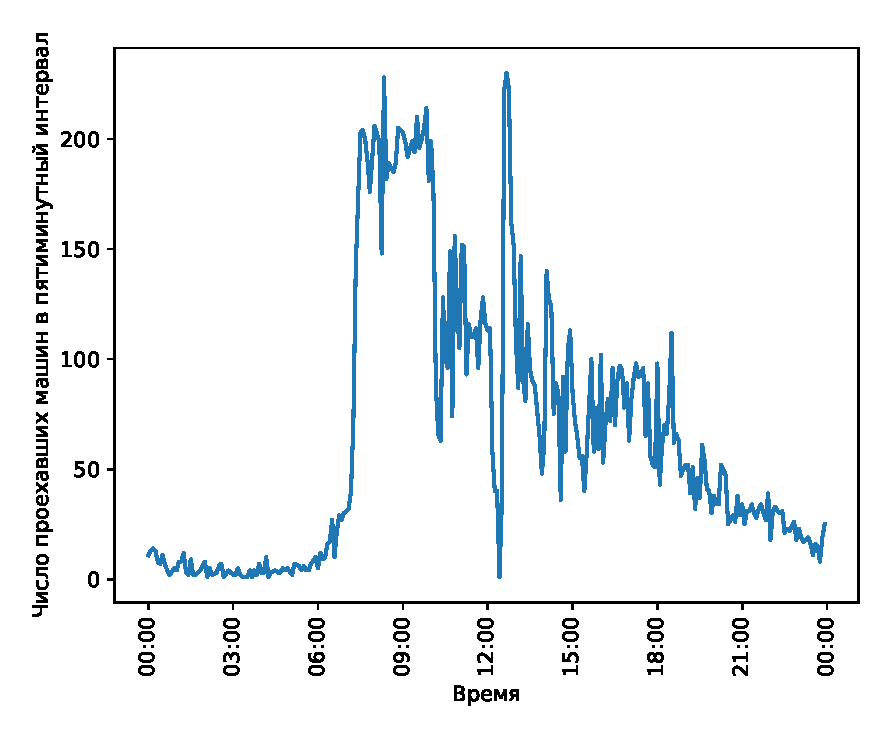
\includegraphics[width=1.0\linewidth]{Detector.eps}
    }
    \caption{Данные с дорожного датчика за один день. Пиковая нагрузка 45 АТС/мин в 8:20.}
    \label{fig:Detector_example}
\end{figure}

Таким образом, в экспериментах функции входного потока на въездах строились так, чтобы походить на данные с реального дорожного детектора и соответствовали информации о пиковой (или средней, если это требовалось) нагрузке на въезде и числу проезжающих по автомагистрали за день АТС.

Как говорилось выше, все въезды также вручную были разделены на два класса:
\begin{enumerate}
  \item Въезды с магистралей по направлению из Москвы, на которых поток АТС нарастает ближе к вечеру.
  \item Въезды с магистралей по направлению в Москву, на которых поток АТС нарастает утром и спадает к вечеру.
\end{enumerate}


\section{Описание данных}
\label{sec::data}
В разделе проводится моделирование внешней стороны Московской кольцевой автомобильной дороги~(МКАД), рис.~\ref{fig:MCAR_map}.
Для построения графа использовалась топология, взятая у компании Яндекс в 2014 г.
Полученная топология, а также увеличенный участок МКАД со съездами и въездами изображены на рис.~\ref{fig:MCAR_topology}.

\begin{figure}[ht]
    \centerfloat{
        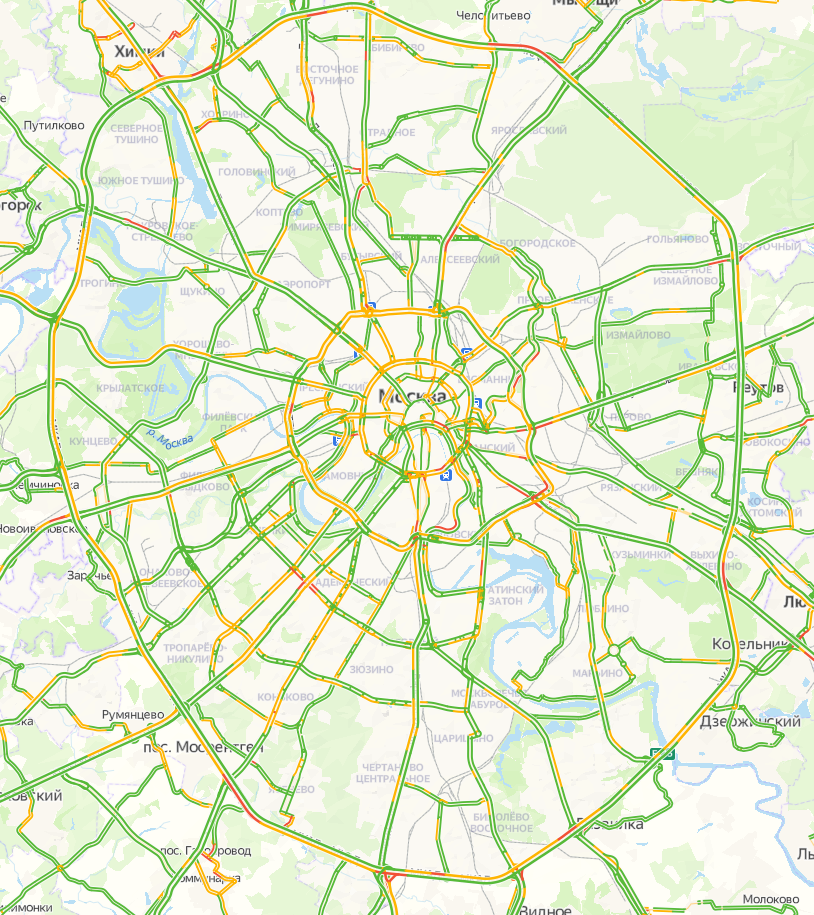
\includegraphics[width=1.0\linewidth]{YandexMap2.png}
    }
    \caption{Типичные пробки по понедельникам в 18:15 на основе статистики сервиса «Яндекс-пробки» транспортной сети Москвы и МКАД, в частности по состоянию на 16.05.21.}
    \label{fig:MCAR_map}
\end{figure}

\begin{figure}[ht]
    \begin{minipage}[b][][b]{0.7045\textwidth}
        \centering
        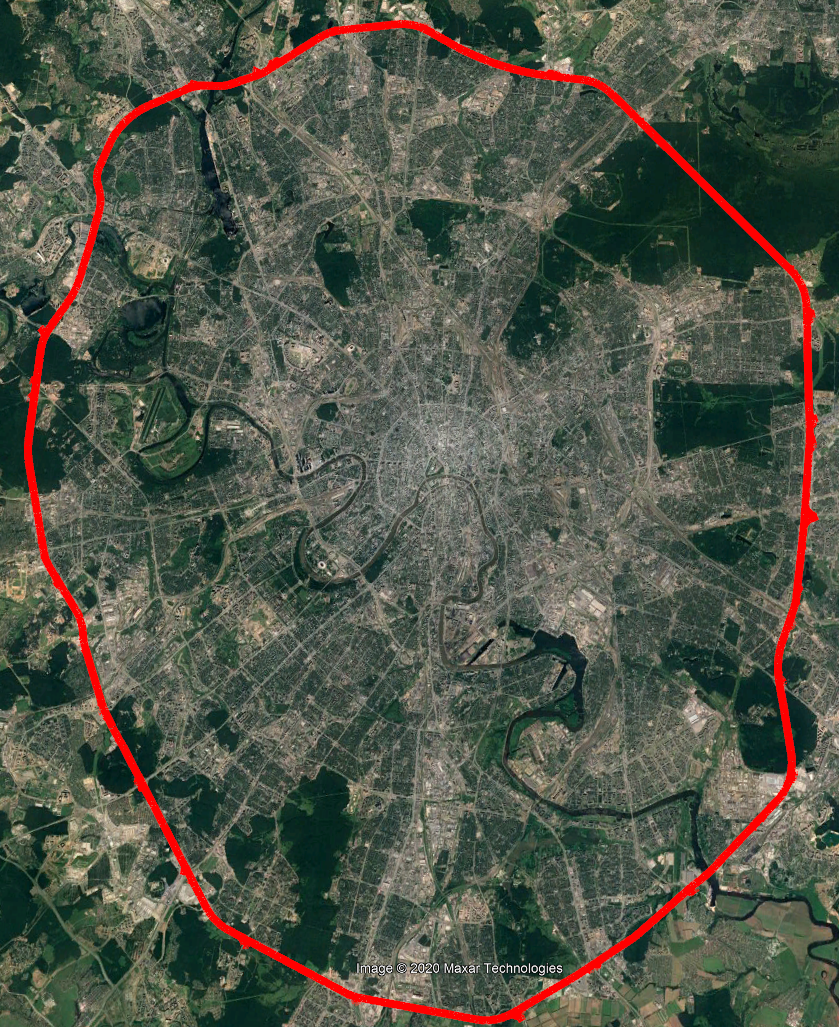
\includegraphics[width=1\linewidth]{YandexMCAR_topology.png} \\ а)
    \end{minipage}
    \hfill
    \begin{minipage}[b][][b]{0.2755\textwidth}
        \centering
        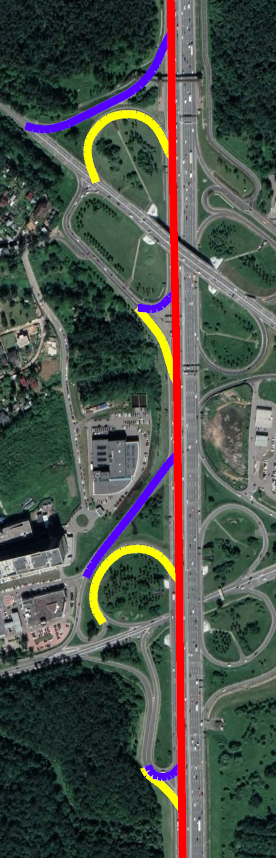
\includegraphics[width=1\linewidth]{YandexMCAR_topology_enter.png} \\ б)
    \end{minipage}

    \caption{а) Вид рассчетного графа МКАД, полученного с помощью топологии компании Яндекс, б) Конфигурация въездов и съездов с МКАД в полученном на основе топологии компании Яндекс графе. Красная линия~--- МКАД, желтая~--- въезды на магистраль, синяя~--- съезды с нее.}
    \label{fig:MCAR_topology}
\end{figure}

В данном разделе во всех экспериментах использовалось несколько фундаментальных диаграмм поток-плотность, полученных анализом реальных данных с дорожных датчиков за 2012 г.
Бралось всего несколько фундаментальных диаграмм эмпирическим образом распределенных между участками МКАД с целью проверки работоспособности модели в ситуации существенно недостаточных для построения всех диаграмм данных.
В следующих разделах будет показан полный эксперимент на основе всех фундаментальных диаграмм поток-плотность для всех сегментов транспортной сети.

\section{Вычислительные эксперименты}
\label{sec::experiments}
Проведены следующие группы вычислительных экспериментов:
\begin{enumerate}
  \item Эксперименты со средней, но продолжительной, пиковой загрузкой на въезды с проверкой эффекта от динамического ограничения входного потока в зависимости от состояния автомагистрали.
  \item Эксперименты с высокой, но непродолжительной, пиковой загрузкой въездов (что более соответствует данным от ЦОДД) с проверкой эффекта от динамического ограничения входного потока в зависимости от состояния автомагистрали.
  \item Эксперименты с длинными въездами с высокой, но непродолжительной, пиковой загрузкой въездов с проверкой эффекта от динамического ограничения входного потока в зависимости от состояния автомагистрали. В данной группе экспериментов максимальная длина очереди на въездах на МКАД увеличена для расчетов времени ожидания на въезде на магистраль без управления въездами и с ним.
\end{enumerate}

В связи с отсутствием реальных данных о числе покидающих автомагистраль транспортных средств в каждый момент времени считаем эту долю фиксированной и выбранной из следующих соображений:
\begin{enumerate}
  \item проезжать более половины МКАД в одну сторону неосмысленно так как в данном случае можно поехать в другую сторону,
  \item на половине МКАД в рассматриваемой модели 32 съезда.
\end{enumerate}
Таким образом, если \(x\)~--- доля съезжающих на каждом съезде АТС, то величина \((1-x)^{30}\) должна быть мала. В экспериментах используется величина \(x = 12\%\).

В каждой группе экспериментов также проводится моделирование ситуации установки светофора на въездах на автомагистраль.
В таком случае алгоритм ограничения входного потока на МКАД выглядит следующим образом:
\begin{itemize}
  \item Для каждого сегмента автомагистрали по направлению движения АТС после рассматриваемого въезда посчитаем плотность автомобилей \(\rho\) на ней.
  \item В зависимости от величины \(\rho_{\text{opt}} - \rho$, где $\rho_{\text{opt}}\)~--- плотность, при которой достигается максимальный поток на рассматриваемом сегменте автомагистрали, входной поток ограничивается на \(l<l_{\text{max}}\) процентов.
  \item Ограничения для каждого из сегментов складываются и получается результирующее понижение входного потока АТС.
\end{itemize}

Важной характеристикой моделируемой системы считаем временные потери на проезд по транспортной сети относительно пустой автомагистрали, т.е. автомагистрали, по которой возможно движение АТС с максимально допустимой скоростью.
Каждую минуту рассчитывается среднее продвижение каждого автомобиля в модели и сравнивается с расстоянием, которое он мог бы преодолеть по пустой магистрали.
Это преобразуется в график временных потерь, который трактуется как время простоя автомобиля в транспортной сети за минуту.

\subsection{Эксперименты со средней загрузкой}
\label{sec:ch5/average}
В данной группе экспериментов въезды считаются однополосными и функции входного потока изображены на рис.~\ref{fig:MCAR_flow_low_3h}.
В данном случае есть два типа въездов на автомагистраль~--- с утренней и вечерней пиковыми загрузками в течение трех часов.
\begin{figure}[ht]
    \begin{minipage}[b][][b]{0.49\textwidth}
        \centering
        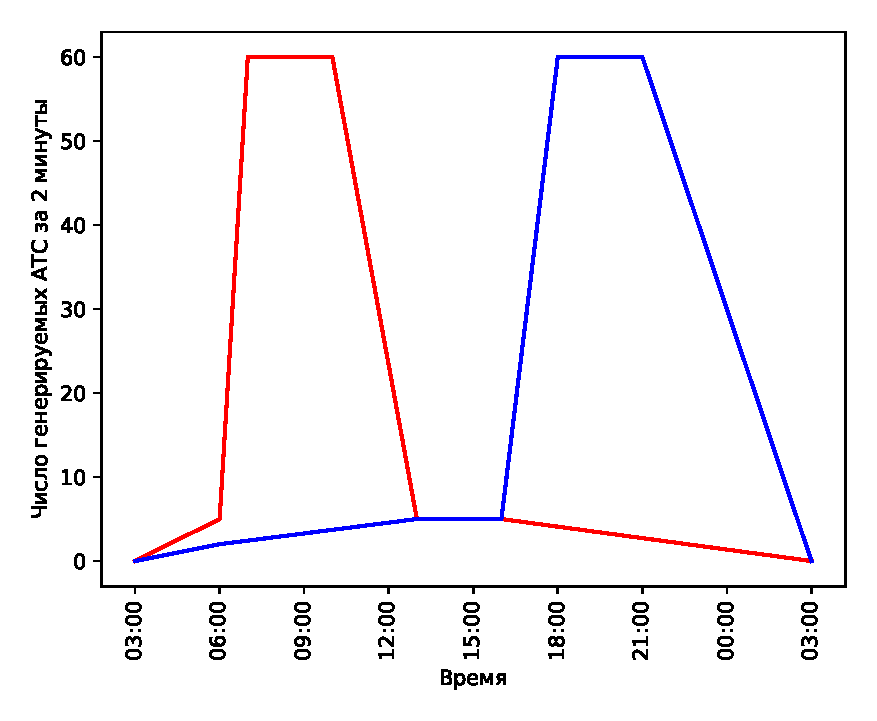
\includegraphics[width=1\linewidth]{MCAR_full_woenters_12_two_types_60_24h_3hmax_Enters_generators.eps}
        \caption{Графики загрузки двух типов въездов~--- с утренней и вечерней пиковыми загрузками в эксперименте со средней загрузкой.}
        \label{fig:MCAR_flow_low_3h}
    \end{minipage}
    \hfill
    \begin{minipage}[b][][b]{0.49\textwidth}
        \centering
        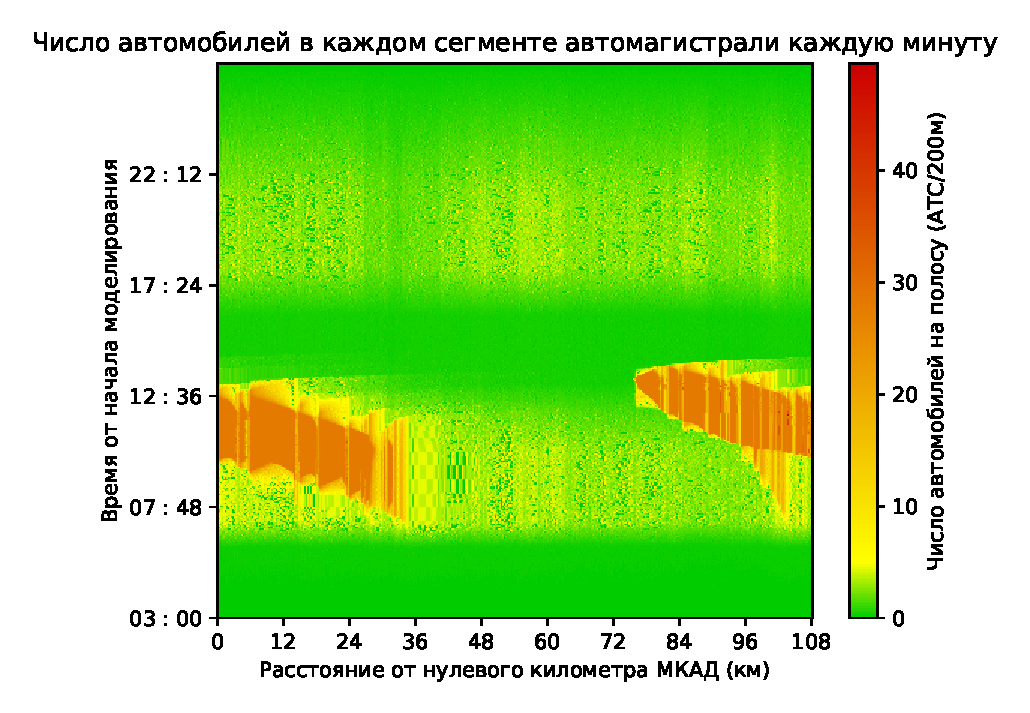
\includegraphics[width=1\linewidth]{MCAR_full_woenters_12_two_types_60_24h_3hmax.eps}
        \caption{Количество автомобилей на полосе в модели транспортной сети за день в эксперименте со средней загрузкой.}
        \label{fig:MCAR_heatmap_low_3h}
    \end{minipage}
\end{figure}

\subsection{Эксперимент без управления въездами}
Результаты моделирования автомагистрали при такой конфигурации въездов представлены на рис.~\ref{fig:MCAR_heatmap_low_3h}.
Число реально въехавших автомобилей и количество проехавших за день по транспортной сети АТС изображены на рис.~\ref{fig:MCAR_entered_low_3h}.
График временных потерь~- на рис.~\ref{fig:MCAR_timeloss_low_3h}.

Видно, что при такой конфигурации входных потоков заторы возникают всего в нескольких местах и потом со временем распространяются по автомагистрали.
Так как пробки успевают исчезнуть к вечеру, то МКАД не останавливается полностью, хотя при меньшей доли съезжающих автомобилей это произойдет.
\begin{figure}[ht]
    \begin{minipage}[b][][b]{0.49\textwidth}
        \centering
        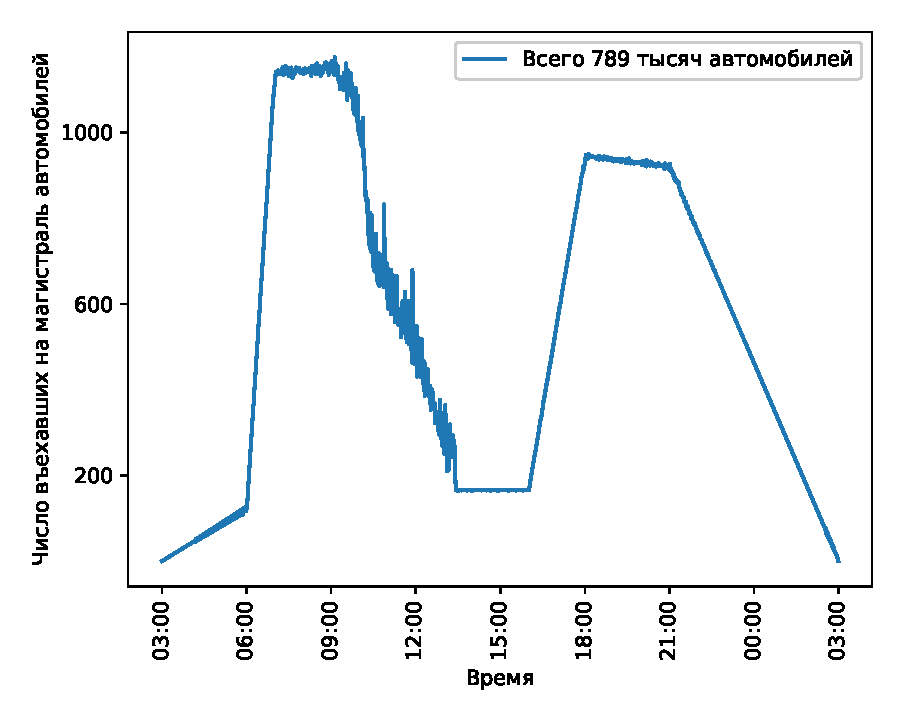
\includegraphics[width=1\linewidth]{MCAR_full_woenters_12_two_types_60_24h_3hmax_Entered.eps}
        \caption{График суммарно въехавшего на автомагистраль со всех въездов числа автомобилей в эксперименте со средней загрузкой.}
        \label{fig:MCAR_entered_low_3h}
    \end{minipage}
    \hfill
    \begin{minipage}[b][][b]{0.49\textwidth}
        \centering
        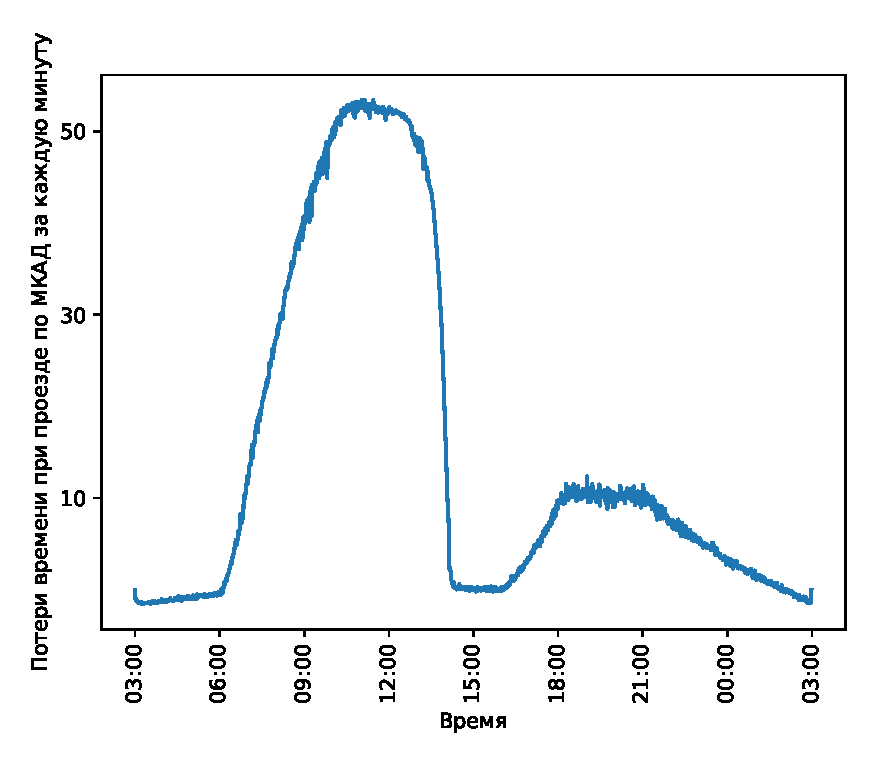
\includegraphics[width=1\linewidth]{MCAR_full_woenters_12_two_types_60_24h_3hmax_Time_to_pass.eps}
        \caption{Временные потери на проезд по автомагистрали в эксперименте со средней загрузкой.}
        \label{fig:MCAR_timeloss_low_3h}
    \end{minipage}
\end{figure}


\subsection{Эксперимент с управлением въездами}
Промоделируем ситуацию, в которой при увеличении потока на автомагистрали будем ограничивать поток с ближайших въездов на автомагистраль искусственно, например с помощью светофора.
В данном эксперименте можем перекрывать въезд вплоть до 80\% в зависимости от плотности автомобилей на магистрали.
Результаты моделирования при такой конфигурации въездов представлены на рис.~\ref{fig:MCAR_heatmap_low_3h_handcontrol}.
Число реально въехавших автомобилей и количество проехавших за день по транспортной сети АТС изображены на рис.~\ref{fig:MCAR_entered_low_3h_handcontrol}.
График временных потерь проезда по всей автомагистрали представлен на рис.~\ref{fig:MCAR_timeloss_low_3h_handcontrol}.
\begin{figure}[ht]
    \centerfloat{
        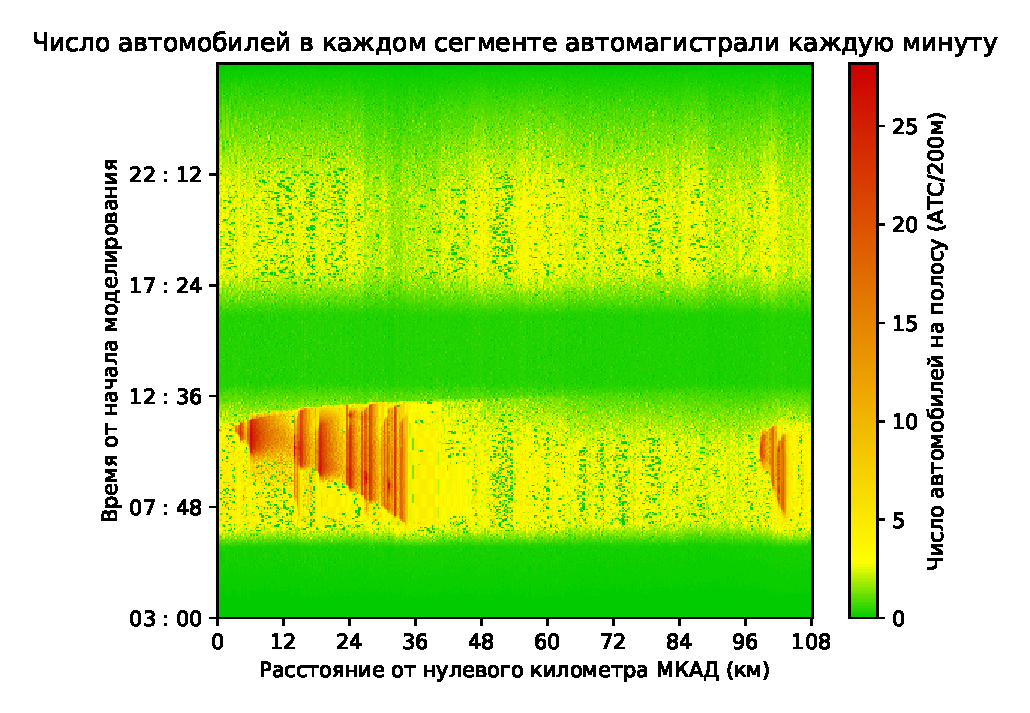
\includegraphics[width=0.8\linewidth]{MCAR_full_woenters_12_two_types_60_24h_3hmax_handcontrol.eps}
    }
    \caption{Количество автомобилей на полосе в модели транспортной сети за день в эксперименте со средней загрузкой с управлением въездами.}
    \label{fig:MCAR_heatmap_low_3h_handcontrol}
\end{figure}

\begin{figure}[ht]
    \begin{minipage}[b][][b]{0.49\textwidth}
        \centering
        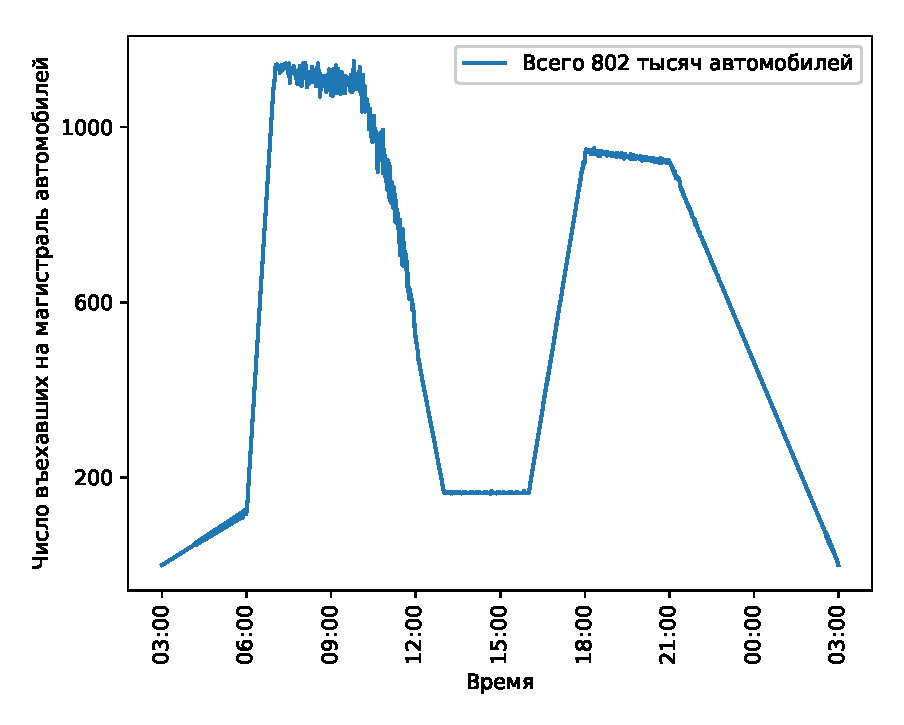
\includegraphics[width=1\linewidth]{MCAR_full_woenters_12_two_types_60_24h_3hmax_handcontrol_Entered.eps}
        \caption{График суммарно въехавшего на автомагистраль со всех въездов числа автомобилей в эксперименте со средней загрузкой с управлением въездами.}
        \label{fig:MCAR_entered_low_3h_handcontrol}
    \end{minipage}
    \hfill
    \begin{minipage}[b][][b]{0.49\textwidth}
        \centering
        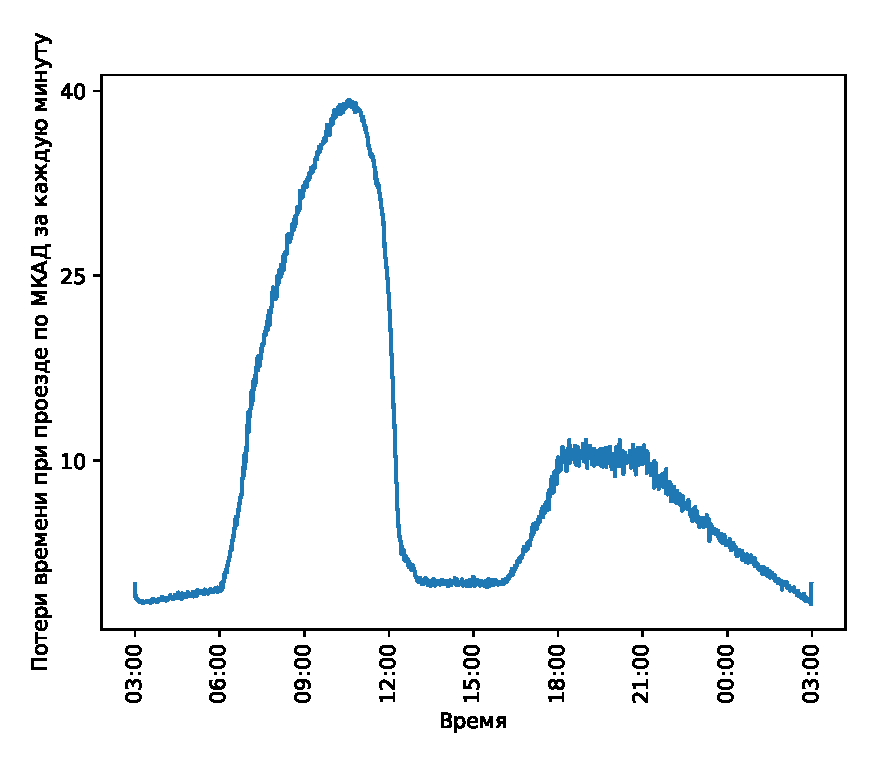
\includegraphics[width=1\linewidth]{MCAR_full_woenters_12_two_types_60_24h_3hmax_handcontrol_Time_to_pass.eps}
        \caption{Временные потери на проезд по автомагистрали в эксперименте со средней загрузкой с управлением въездами.}
        \label{fig:MCAR_timeloss_low_3h_handcontrol}
    \end{minipage}
\end{figure}

На графиках видно уменьшение времени затора на МКАД, а также небольшое увеличение числа проехавших автомобилей.
Однако временные потери на проезд по автомагистрали значительно снизились.
Интегральная разность между графиками временных потерь на рис.~\ref{fig:MCAR_timeloss_low_3h}~и~\ref{fig:MCAR_timeloss_low_3h_handcontrol} составляет около $4,5$ минут.


\section{Эксперименты с высокой загрузкой}
\label{sec:ch5/hight}
В данной группе экспериментов въезды считаются двухполосными и функции входного потока изображены на рис.~\ref{fig:MCAR_flow_hight_3h}.
В данном случае есть два типа въездов на автомагистраль~--- с утренней и вечерней пиковыми загрузками в течение трех часов.
\begin{figure}[ht]
    \begin{minipage}[b][][b]{0.49\textwidth}
        \centering
        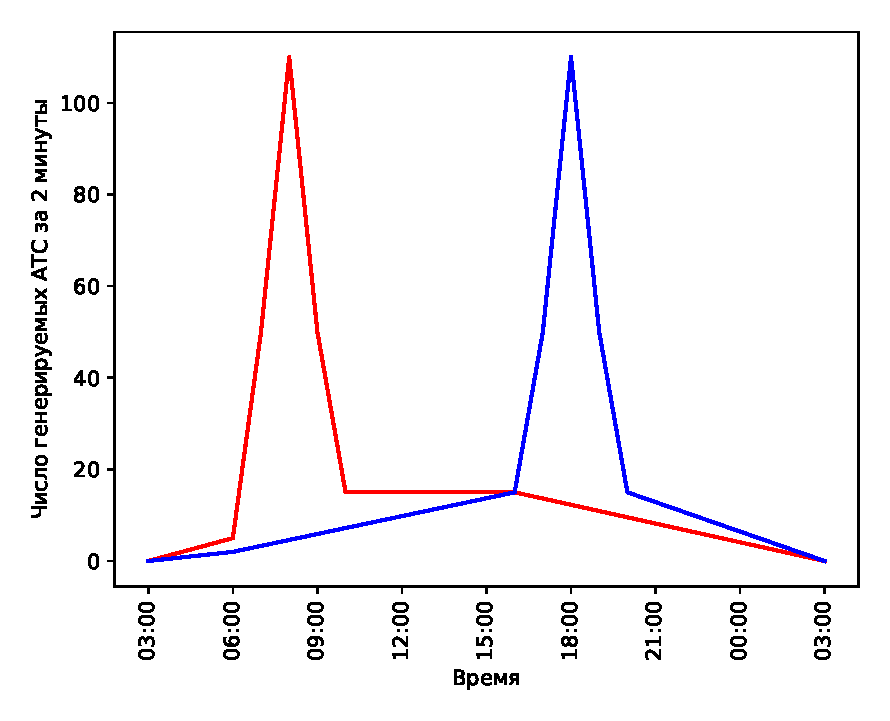
\includegraphics[width=1\linewidth]{MCAR_full_woenters_12_two_types_110_24h_3h_Enters_generators.eps}
        \caption{Графики загрузки двух типов въездов~--- с утренней и вечерней пиковыми загрузками в эксперименте с высокой загрузкой.}
        \label{fig:MCAR_flow_hight_3h}
    \end{minipage}
    \hfill
    \begin{minipage}[b][][b]{0.49\textwidth}
        \centering
        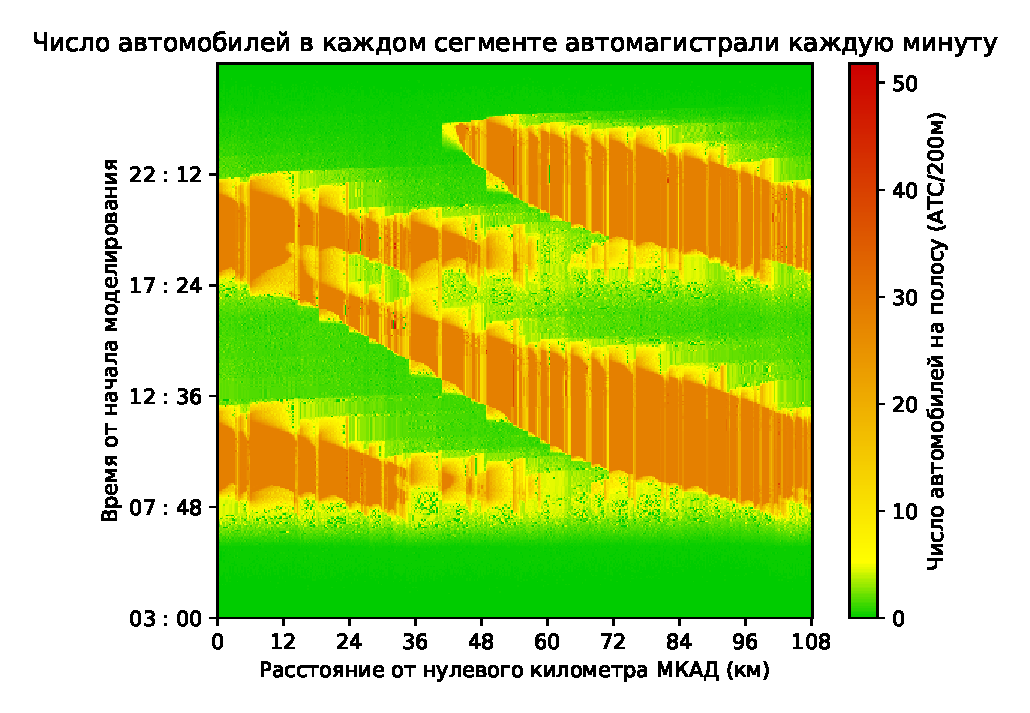
\includegraphics[width=1\linewidth]{MCAR_full_woenters_12_two_types_110_24h_3h.eps}
        \caption{Количество автомобилей на полосу в модели транспортной сети за день в эксперименте с высокой загрузкой.}
        \label{fig:MCAR_heatmap_hight_3h}
    \end{minipage}
\end{figure}

\subsection{Эксперимент без управления въездами}
Результаты моделирования при такой конфигурации въездов представлены на рис.~\ref{fig:MCAR_heatmap_hight_3h}.
Видно, что в данной конфигурации потоков на въездах заторные движения образуются по всей протяженности автомагистрали, объединяясь впоследствии в один большой. В данном эксперименте МКАД практически полностью занят пробкой с утра до вечера.
На рис.~\ref{fig:MCAR_entered_hight_3h} показано число реально въехавших автомобилей и количество проехавших за день по магистрали АТС.
График временных потерь проезда по всей автомагистрали представлен на рис.~\ref{fig:MCAR_timeloss_hight_3h}.

\begin{figure}[ht]
    \begin{minipage}[b][][b]{0.49\textwidth}
        \centering
        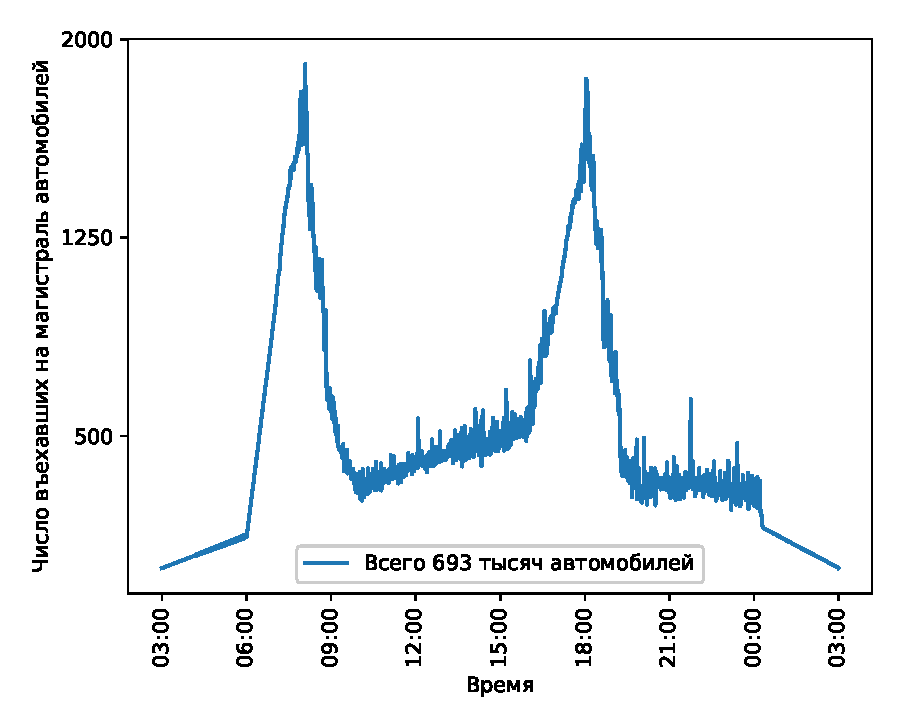
\includegraphics[width=1\linewidth]{MCAR_full_woenters_12_two_types_110_24h_3h_Entered.eps}
        \caption{График суммарно въехавшего на автомагистраль со всех въездов числа автомобилей в эксперименте с высокой загрузкой.}
        \label{fig:MCAR_entered_hight_3h}
    \end{minipage}
    \hfill
    \begin{minipage}[b][][b]{0.49\textwidth}
        \centering
        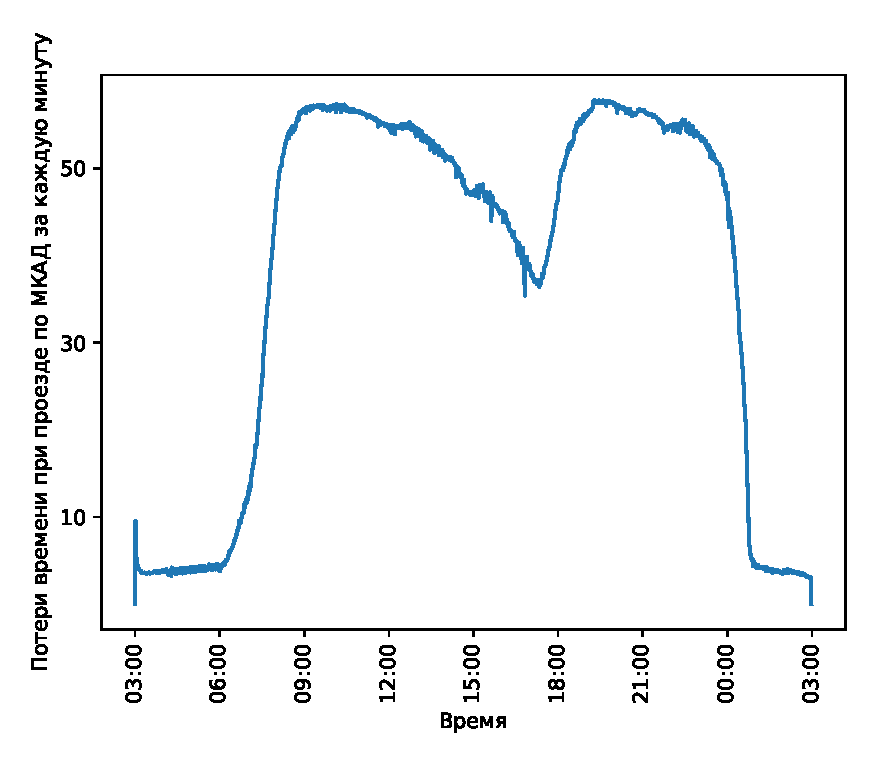
\includegraphics[width=1\linewidth]{MCAR_full_woenters_12_two_types_110_24h_3h_Time_to_pass.eps}
        \caption{Временные потери на проезд по автомагистрали в эксперименте с высокой загрузкой.}
        \label{fig:MCAR_timeloss_hight_3h}
    \end{minipage}
\end{figure}


\subsection{Эксперимент с управлением въездами}
В данном эксперименте с управлением въездами также перекрываем въезды вплоть до 80\% в зависимости от плотности автомобилей на магистрали.
Результаты моделирования, число въехавших автомобилей и график временных потерь при проезде по магистрали изображены на рис.~\ref{fig:MCAR_heatmap_low_3h_handcontrol},~\ref{fig:MCAR_entered_low_3h_handcontrol} и~\ref{fig:MCAR_timeloss_low_3h_handcontrol} соответственно.
\begin{figure}[ht]
    \centerfloat{
        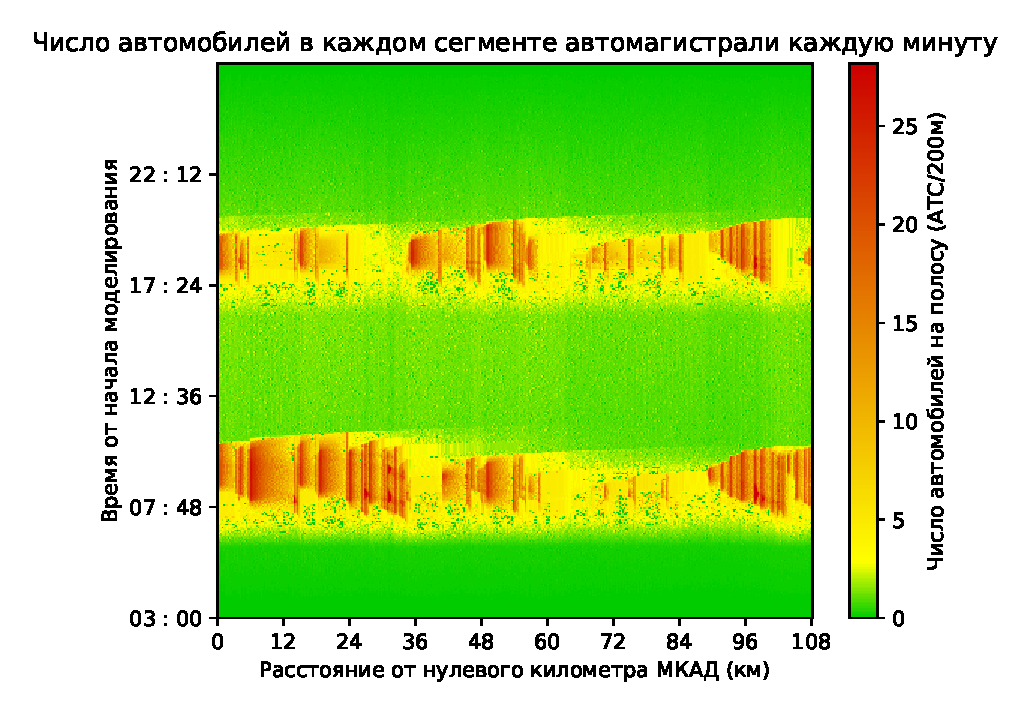
\includegraphics[width=0.8\linewidth]{MCAR_full_woenters_12_two_types_110_24h_3h_handcontrol.eps}
    }
    \caption{Количество автомобилей на полосе в модели транспортной сети за день в эксперименте с высокой загрузкой с управлением въездами.}
    \label{fig:MCAR_heatmap_hight_3h_handcontrol}
\end{figure}

\begin{figure}[ht]
    \begin{minipage}[b][][b]{0.49\textwidth}
        \centering
        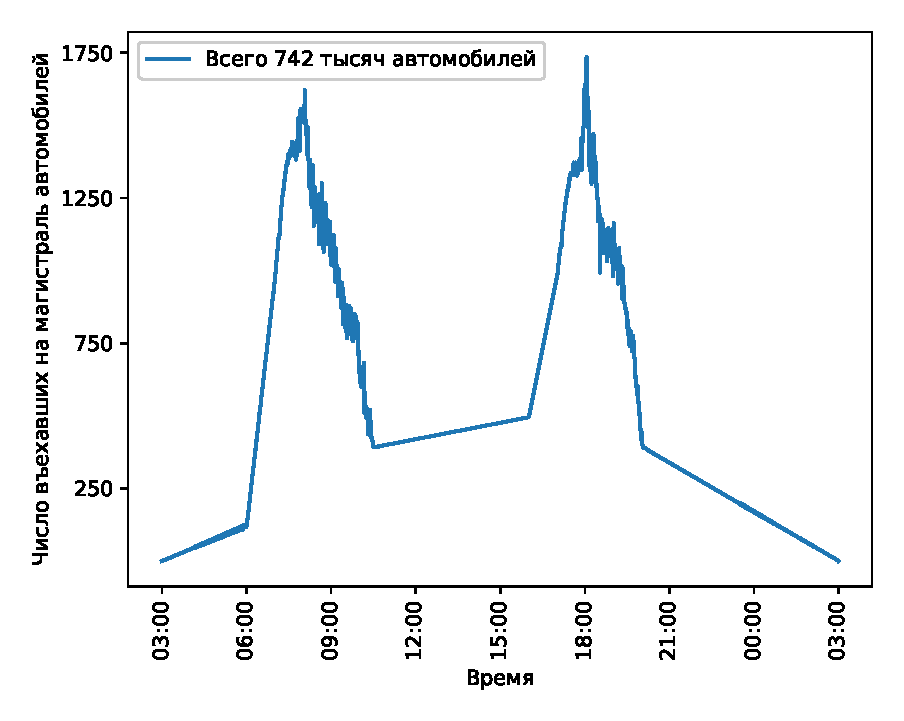
\includegraphics[width=1\linewidth]{MCAR_full_woenters_12_two_types_110_24h_3h_handcontrol_Entered.eps}
        \caption{График суммарно въехавшего на автомагистраль со всех въездов числа автомобилей в эксперименте с высокой загрузкой с управлением въездами.}
        \label{fig:MCAR_entered_hight_3h_handcontrol}
    \end{minipage}
    \hfill
    \begin{minipage}[b][][b]{0.49\textwidth}
        \centering
        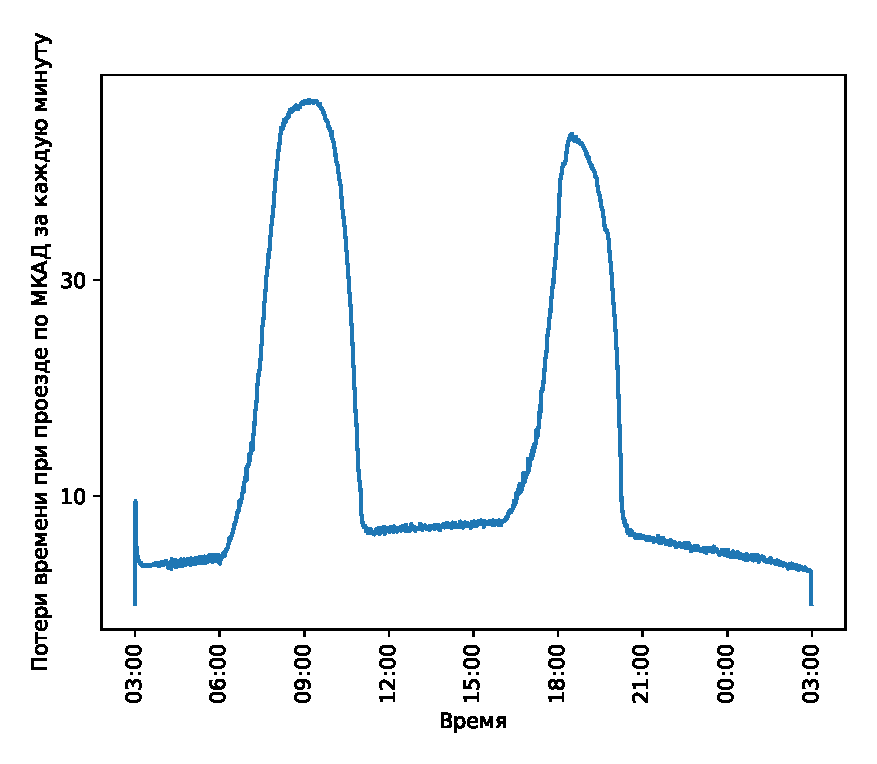
\includegraphics[width=1\linewidth]{MCAR_full_woenters_12_two_types_110_24h_3h_handcontrol_Time_to_pass.eps}
        \caption{Временные потери на проезд по автомагистрали в эксперименте с высокой загрузкой с управлением въездами.}
        \label{fig:MCAR_timeloss_hight_3h_handcontrol}
    \end{minipage}
\end{figure}

На графиках видно уменьшение времени затора на МКАД, а также небольшое увеличение числа проехавших автомобилей.
Хотя число проехавших по МКАД автомобилей увеличилось незначительно, временные потери на проезд по автомагистрали сильно снизились, а временной интервал затрудненного движения уменьшился.
Интегральная разность между графиками на рис.~\ref{fig:MCAR_timeloss_hight_3h}~и~\ref{fig:MCAR_timeloss_hight_3h_handcontrol} составляет чуть более $18$ минут.

\section{Эксперименты с высокой загрузкой с длинными въездами}
В данной группе экспериментов функции входного потока соответствуют потоку в предыдущем эксперименте и изображены на рис.~\ref{fig:MCAR_flow_hight_3h}.
В данном случае у нас есть два типа въездов на автомагистраль~--- с утренней и вечерней пиковыми загрузками в течение трех часов.
Въезды на автомагистраль~- все протяженностью в $6$ километров в отличие от уже проведенных экспериментов, в которых их длина бралась $2$ километра.

В данном разделе приведем все результирующие графики парами.
Результаты моделирования представлены на рис.~\ref{fig:MCAR_heatmap_hight_3h_6km}.
Число реально въехавших автомобилей и количество проехавших за день по магистрали АТС изображены на рис.~\ref{fig:MCAR_entered_hight_3h_6km}.
График временных потерь проезда по всей автомагистрали представлен на рис.~\ref{fig:MCAR_timeloss_hight_3h_6km}.
График временных потерь въезда на автомагистрали относительно пустой транспортной сети показан на рис.~\ref{fig:MCAR_timeloss_enter_hight_3h_6km}.

В эксперименте видно, что из-за большого числа автомобилей, ожидающих въезда на МКАД без управления въездами, автомагистраль полностью забивается и не успевает освободиться до конца моделирования.
Поскольку динамическое управление въездами не позволяет пробке поддерживаться за счет ограничения входного потока на магистраль, наблюдается значительное улучшение состояния магистрали и сильная локализация затора во времени.

Интегральная разность между графиками на рис.~\ref{fig:MCAR_timeloss_enter_hight_3h_6km} составляет чуть более $26$ минут.
Однако имеет смысл не учитывать сугубо экстремальную вечернюю ситуацию с практически полной остановкой автомагистрали. В этом случае при расчете интеграла до 15:00 задержка ожидания проезда по МКАД составит около $7$ минут за половину суток.

\begin{figure}[ht]
    \begin{minipage}[b][][b]{0.49\textwidth}
        \centering
        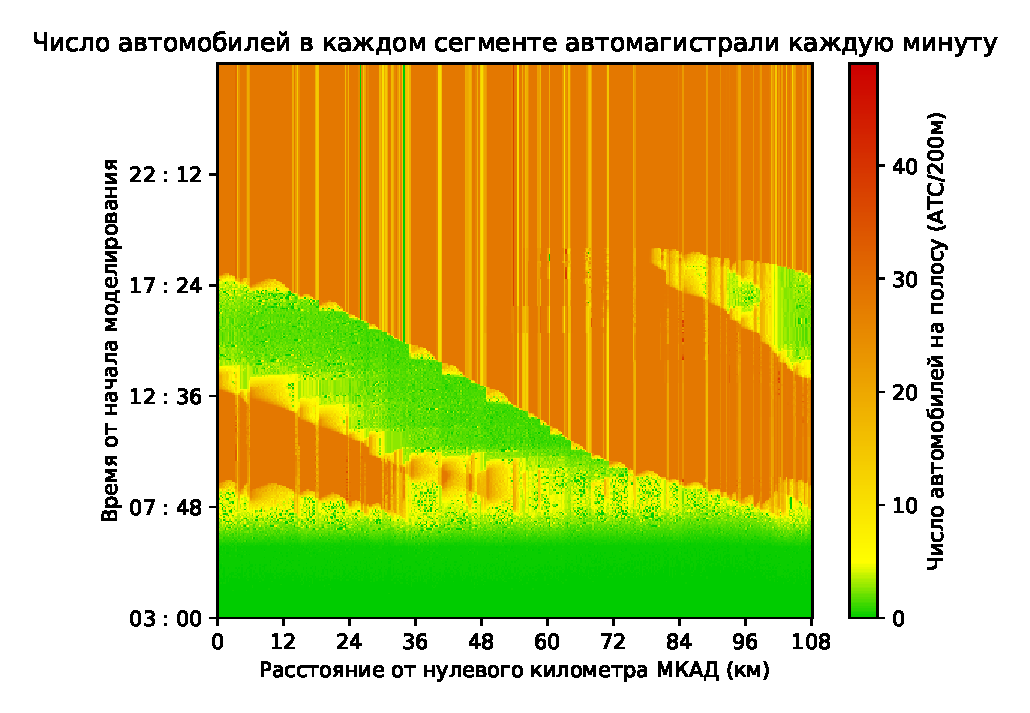
\includegraphics[width=1\linewidth]{MCAR_full_woenters_12_two_types_110_24h_3h_6km.eps} \\ а) Без управления въездами
    \end{minipage}
    \hfill
    \begin{minipage}[b][][b]{0.49\textwidth}
        \centering
        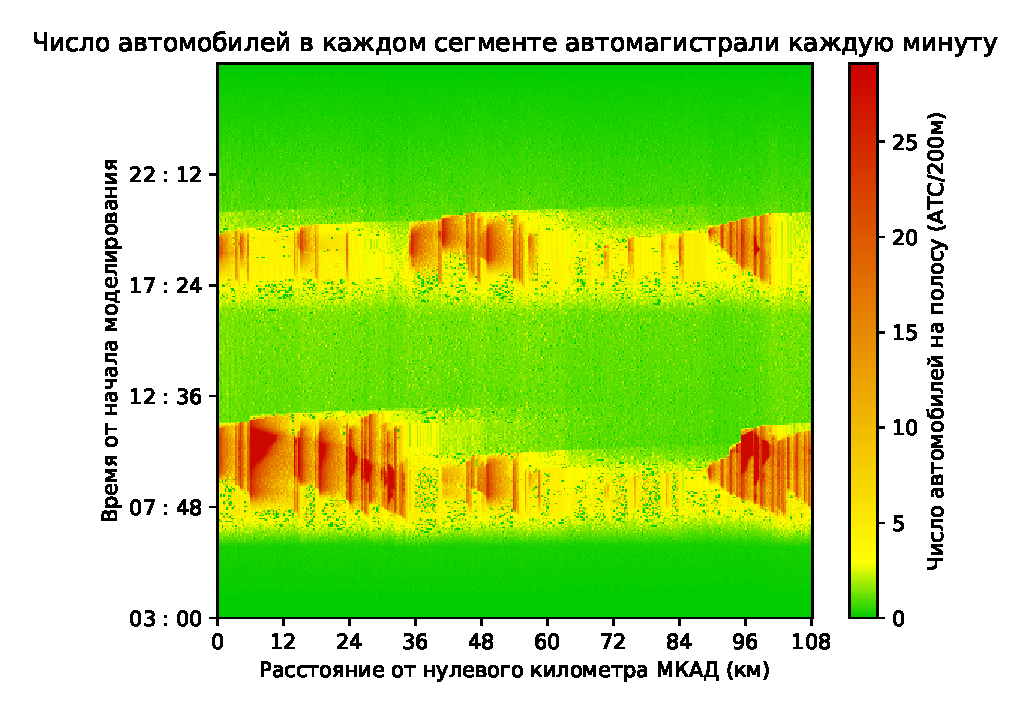
\includegraphics[width=1\linewidth]{MCAR_full_woenters_12_two_types_110_24h_3h_6km_handcontrol.eps} \\ б) С управлением въездами
    \end{minipage}

    \caption{Количество автомобилей на полосу в модели транспортной сети за день в эксперименте с высокой загрузкой.}
    \label{fig:MCAR_heatmap_hight_3h_6km}
\end{figure}

\begin{figure}[ht]
    \begin{minipage}[b][][b]{.49\textwidth}
        \centering
        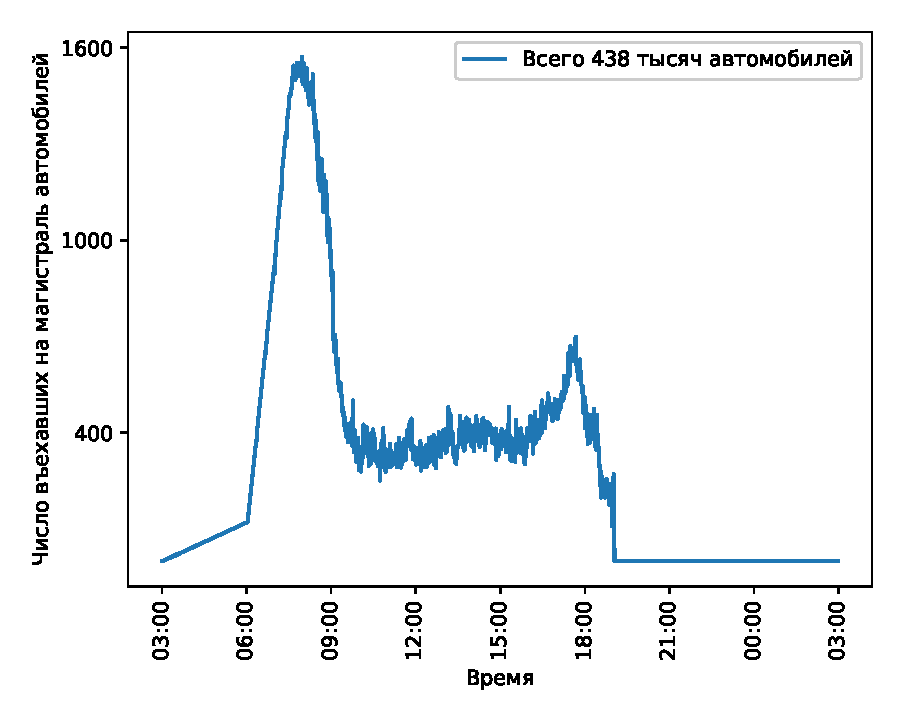
\includegraphics[width=1\linewidth]{MCAR_full_woenters_12_two_types_110_24h_3h_6km_Entered.eps} \\ а) Без управления въездами
    \end{minipage}
    \hfill
    \begin{minipage}[b][][b]{.49\textwidth}
        \centering
        \includegraphics[width=1\linewidth]{MCAR_full_woenters_12_two_types_110_24h_3h_6km_handcontrol_Entered.eps} \\ б) С управлением въездами
    \end{minipage}

    \caption{Графики суммарно въехавшего на автомагистраль со всех въездов числа автомобилей в эксперименте с высокой загрузкой.}
    \label{fig:MCAR_entered_hight_3h_6km}
\end{figure}


\begin{figure}[ht]
    \begin{minipage}[b][][b]{.49\textwidth}
        \centering
        \includegraphics[width=1\linewidth]{MCAR_full_woenters_12_two_types_110_24h_3h_6km_Time_to_pass.eps} \\ а) Без управления въездами
    \end{minipage}
    \hfill
    \begin{minipage}[b][][b]{.49\textwidth}
        \centering
        \includegraphics[width=1\linewidth]{MCAR_full_woenters_12_two_types_110_24h_3h_6km_handcontrol_Time_to_pass.eps} \\ б) С управлением въездами
    \end{minipage}

    \caption{Временные потери на проезд по автомагистрали в эксперименте с высокой загрузкой.}
    \label{fig:MCAR_timeloss_hight_3h_6km}
\end{figure}

\begin{figure}[ht]
    \begin{minipage}[b][][b]{.49\textwidth}
        \centering
        \includegraphics[width=1\linewidth]{MCAR_full_woenters_12_two_types_110_24h_3h_6km_Time_to_enter.eps}  \\ а) Без управления въездами
    \end{minipage}
    \hfill
    \begin{minipage}[b][][b]{.49\textwidth}
        \centering
        \includegraphics[width=1\linewidth]{MCAR_full_woenters_12_two_types_110_24h_3h_6km_handcontrol_Time_to_enter.eps}  \\ b) С управлением въездами
    \end{minipage}

    \caption{Временные потери на въезд на автомагистраль в эксперименте с высокой загрузкой.}
    \label{fig:MCAR_timeloss_enter_hight_3h_6km}
\end{figure}



\chapter{Моделирование МКАД с вычислением всех фундаментальных диаграмм}\label{sec:ch6}
В данном разделе описываются эксперименты, аналогичные проведенным в разделе~\ref{sec::experiments} однако теперь для каждого сегмента МКАД была рассчитана соответствующая ему фундаментальная диаграмма на основе данных с дорожных датчиков
расположенных над этим сегментом либо рядом с ним.
Проводятся следующие группы экспериментов:
\begin{enumerate}
  \item Эксперименты со средней, но продолжительной, пиковой загрузкой на въезды с проверкой эффекта от динамического ограничения входного потока в зависимости от состояния автомагистрали.
  \item Эксперименты с высокой, но непродолжительной, пиковой загрузкой въездов (что более соответствует данным от ЦОДД) с проверкой эффекта от динамического ограничения входного потока в зависимости от состояния автомагистрали.
\end{enumerate}

В данном разделе принимаются все те же предположения что и в разделе~\ref{sec::experiments}, а конкретно~--- доля съезжающих автомобилей равна \(12\%\), а управление въездами происходит по аналогичному алгоритму:
\begin{itemize}
  \item Для каждого сегмента автомагистрали по направлению движения АТС после рассматриваемого въезда посчитаем плотность автомобилей \(\rho\) на ней.
  \item В зависимости от величины \(\rho_{\text{opt}} - \rho$, где $\rho_{\text{opt}}\)~--- плотность, при которой достигается максимальный поток на рассматриваемом сегменте автомагистрали, входной поток ограничивается на \(l<l_{\text{max}}\) процентов.
  \item Ограничения для каждого из сегментов складываются и получается результирующее понижение входного потока АТС.
\end{itemize}

\section{Эксперименты со средней загрузкой}
\label{sec:ch6/average_FD}
В данной группе экспериментов въезды считаются однополосными и функции входного потока изображены на рис.~\ref{fig:MCAR_flow_low_3h}.
В данном случае есть два типа въездов на автомагистраль~--- с утренней и вечерней пиковыми загрузками в течение трех часов.
\begin{figure}[ht]
    \centerfloat{
        \includegraphics[width=0.8\linewidth]{MCAR_full_woenters_12_two_types_60_24h_3hmax_fullFD.eps}
    }
    \caption{Количество автомобилей на полосе в модели транспортной сети за день в эксперименте со средней загрузкой с расчетом всех фундаментальных диаграмм.}
    \label{fig:MCAR_heatmap_low_3h_FD}
\end{figure}

\subsection{Эксперимент без управления въездами}
Результаты моделирования автомагистрали при такой конфигурации въездов представлены на рис.~\ref{fig:MCAR_heatmap_low_3h_FD}.
Число реально въехавших автомобилей и количество проехавших за день по транспортной сети АТС изображены на рис.~\ref{fig:MCAR_entered_low_3h_FD}.
График временных потерь~- на рис.~\ref{fig:MCAR_timeloss_low_3h_FD}.

Видно, что при такой конфигурации входных потоков заторы возникают всего в нескольких местах и потом со временем распространяются по автомагистрали.
Так как пробки успевают исчезнуть к вечеру, то МКАД не останавливается полностью, хотя при меньшей доли съезжающих автомобилей это произойдет.
В сравнении с аналогичным экспериментом из предыдущего раздела пробка исчезает быстрее при спаде входного потока АТС.
\begin{figure}[ht]
    \begin{minipage}[b][][b]{0.49\textwidth}
        \centering
        \includegraphics[width=1\linewidth]{MCAR_full_woenters_12_two_types_60_24h_3hmax_fullFD_Entered.eps}
        \caption{График суммарно въехавшего на автомагистраль со всех въездов числа автомобилей в эксперименте со средней загрузкой с расчетом всех фундаментальных диаграмм.}
        \label{fig:MCAR_entered_low_3h_FD}
    \end{minipage}
    \hfill
    \begin{minipage}[b][][b]{0.49\textwidth}
        \centering
        \includegraphics[width=1\linewidth]{MCAR_full_woenters_12_two_types_60_24h_3hmax_fullFD_Time_to_pass.eps}
        \caption{Временные потери на проезд по автомагистрали в эксперименте со средней загрузкой с расчетом всех фундаментальных диаграмм.}
        \label{fig:MCAR_timeloss_low_3h_FD}
    \end{minipage}
\end{figure}


\subsection{Эксперимент с управлением въездами}
Аналогично предыдущему разделу промоделируем ситуацию светофорного управления въездами с возможностью перекрывать вплоть до 80\% входного потока.
Результаты моделирования при такой конфигурации въездов представлены на рис.~\ref{fig:MCAR_heatmap_low_3h_handcontrol_FD}.
Число реально въехавших автомобилей и количество проехавших за день по транспортной сети АТС изображены на рис.~\ref{fig:MCAR_entered_low_3h_handcontrol_FD}.
График временных потерь проезда по всей автомагистрали представлен на рис.~\ref{fig:MCAR_timeloss_low_3h_handcontrol_FD}.
\begin{figure}[ht]
    \centerfloat{
        \includegraphics[width=0.8\linewidth]{MCAR_full_woenters_12_two_types_60_24h_3hmax_fullFD_handcontrol.eps}
    }
    \caption{Количество автомобилей на полосе в модели транспортной сети за день в эксперименте со средней загрузкой с управлением въездами с расчетом всех фундаментальных диаграмм.}
    \label{fig:MCAR_heatmap_low_3h_handcontrol_FD}
\end{figure}

\begin{figure}[ht]
    \begin{minipage}[b][][b]{0.49\textwidth}
        \centering
        \includegraphics[width=1\linewidth]{MCAR_full_woenters_12_two_types_60_24h_3hmax_fullFD_handcontrol_Entered.eps}
        \caption{График суммарно въехавшего на автомагистраль со всех въездов числа автомобилей в эксперименте со средней загрузкой с управлением въездами с расчетом всех фундаментальных диаграмм.}
        \label{fig:MCAR_entered_low_3h_handcontrol_FD}
    \end{minipage}
    \hfill
    \begin{minipage}[b][][b]{0.49\textwidth}
        \centering
        \includegraphics[width=1\linewidth]{MCAR_full_woenters_12_two_types_60_24h_3hmax_fullFD_handcontrol_Time_to_pass.eps}
        \caption{Временные потери на проезд по автомагистрали в эксперименте со средней загрузкой с управлением въездами с расчетом всех фундаментальных диаграмм.}
        \label{fig:MCAR_timeloss_low_3h_handcontrol_FD}
    \end{minipage}
\end{figure}

На графиках видно уменьшение времени затора на МКАД, а также небольшое увеличение числа проехавших автомобилей.
Однако временные потери на проезд по автомагистрали значительно снизились.
Интегральная разность между графиками временных потерь на рис.~\ref{fig:MCAR_timeloss_low_3h_FD}~и~\ref{fig:MCAR_timeloss_low_3h_handcontrol_FD} составляет около $1$ минуты.
Видно, что при низкой загрузке и более аккуратном моделировании с учетом всех фундаментальных диаграмм эффективность управления въездами достаточно сильно упала.


\section{Эксперименты с высокой загрузкой}
\label{sec:ch6/hight_FD}
В данной группе экспериментов въезды считаются двухполосными и функции входного потока изображены на рис.~\ref{fig:MCAR_flow_hight_3h}.
В данном случае есть два типа въездов на автомагистраль~--- с утренней и вечерней пиковыми загрузками в течение трех часов.

\begin{figure}[ht]
    \centerfloat{
        \includegraphics[width=0.8\linewidth]{MCAR_full_woenters_12_two_types_110_24h_3h_fullFD.eps}
    }
    \caption{Количество автомобилей на полосу в модели транспортной сети за день в эксперименте с высокой загрузкой с расчетом всех фундаментальных диаграмм.}
    \label{fig:MCAR_heatmap_hight_3h_FD}
\end{figure}


\subsection{Эксперимент без управления въездами}
Результаты моделирования при такой конфигурации въездов представлены на рис.~\ref{fig:MCAR_heatmap_hight_3h_FD}.
Видно, что в данной конфигурации потоков на въездах заторные движения образуются по всей протяженности автомагистрали, объединяясь впоследствии в один большой.
В данном эксперименте, аналогично эксперименту из предыдущего раздела, МКАД практически полностью занят пробкой с утра до вечера.
На рис.~\ref{fig:MCAR_entered_hight_3h} показано число реально въехавших автомобилей и количество проехавших за день по магистрали АТС.
График временных потерь проезда по всей автомагистрали представлен на рис.~\ref{fig:MCAR_timeloss_hight_3h_FD}.

\begin{figure}[ht]
    \begin{minipage}[b][][b]{0.49\textwidth}
        \centering
        \includegraphics[width=1\linewidth]{MCAR_full_woenters_12_two_types_110_24h_3h_fullFD_Entered.eps}
        \caption{График суммарно въехавшего на автомагистраль со всех въездов числа автомобилей в эксперименте с высокой загрузкой с расчетом всех фундаментальных диаграмм.}
        \label{fig:MCAR_entered_hight_3h_FD}
    \end{minipage}
    \hfill
    \begin{minipage}[b][][b]{0.49\textwidth}
        \centering
        \includegraphics[width=1\linewidth]{MCAR_full_woenters_12_two_types_110_24h_3h_fullFD_Time_to_pass.eps}
        \caption{Временные потери на проезд по автомагистрали в эксперименте с высокой загрузкой с расчетом всех фундаментальных диаграмм.}
        \label{fig:MCAR_timeloss_hight_3h_FD}
    \end{minipage}
\end{figure}


\subsection{Эксперимент с управлением въездами}
В данном эксперименте с управлением въездами также перекрываем въезды вплоть до 80\% в зависимости от плотности автомобилей на магистрали.
Результаты моделирования, число въехавших автомобилей и график временных потерь при проезде по магистрали изображены на рис.~\ref{fig:MCAR_heatmap_low_3h_handcontrol},~\ref{fig:MCAR_entered_low_3h_handcontrol} и~\ref{fig:MCAR_timeloss_low_3h_handcontrol} соответственно.
\begin{figure}[ht]
    \centerfloat{
        \includegraphics[width=0.8\linewidth]{MCAR_full_woenters_12_two_types_110_24h_3h_fullFD_handcontrol.eps}
    }
    \caption{Количество автомобилей на полосе в модели транспортной сети за день в эксперименте с высокой загрузкой с управлением въездами с расчетом всех фундаментальных диаграмм.}
    \label{fig:MCAR_heatmap_hight_3h_handcontrol_FD}
\end{figure}

\begin{figure}[ht]
    \begin{minipage}[b][][b]{0.49\textwidth}
        \centering
        \includegraphics[width=1\linewidth]{MCAR_full_woenters_12_two_types_110_24h_3h_fullFD_handcontrol_Entered.eps}
        \caption{График суммарно въехавшего на автомагистраль со всех въездов числа автомобилей в эксперименте с высокой загрузкой с управлением въездами с расчетом всех фундаментальных диаграмм.}
        \label{fig:MCAR_entered_hight_3h_handcontrol_FD}
    \end{minipage}
    \hfill
    \begin{minipage}[b][][b]{0.49\textwidth}
        \centering
        \includegraphics[width=1\linewidth]{MCAR_full_woenters_12_two_types_110_24h_3h_fullFD_handcontrol_Time_to_pass.eps}
        \caption{Временные потери на проезд по автомагистрали в эксперименте с высокой загрузкой с управлением въездами с расчетом всех фундаментальных диаграмм.}
        \label{fig:MCAR_timeloss_hight_3h_handcontrol_FD}
    \end{minipage}
\end{figure}

На графиках видно уменьшение времени затора на МКАД, а также небольшое увеличение числа проехавших автомобилей.
Хотя число проехавших по МКАД автомобилей увеличилось незначительно, временные потери на проезд по автомагистрали сильно снизились, а временной интервал затрудненного движения уменьшился.
Интегральная разность между графиками на рис.~\ref{fig:MCAR_timeloss_hight_3h_FD}~и~\ref{fig:MCAR_timeloss_hight_3h_handcontrol_FD} составляет ровно \(14\) минут.


\section{Сравнение с экспериментами с несколькими фундаментальными диаграммами}
Видно, что модель показала свою устойчивость относительно точности расчета фундаментальных диаграмм.
Несмотря на то, что результаты изменились, общая картина формирования и распространения затора в модели МКАД осталась неизменна.

Эксперименты из разделов~\ref{sec:ch5/average} и~\ref{sec:ch6/average_FD} показывают схожую картину МКАД в течении дня.
Однако, ввиду более аккуратных расчетов МКАД при средней загрузке сам по себе оказывается менее нагружен, а заторное состояние наблюдается меньшее время.
Таким образом даже без управления въездами состояние МКАДа удовлетворительно для проезда и преимущества от управления в этом варианте минимальные~--- всего одна минута.

В эксперименте с высокой загрузкой на въездах~\ref{sec:ch6/hight_FD} преимущество от управления все еще существенное~--- \(14\) минут.
Это меньше чем в эксперименте из раздела~\ref{sec:ch5/hight} на \(4\) минуты, но все еще очень существенно.
Тут мы также наблюдаем небольшие изменения в структуре распространения заторов.

Окончательно, для детального моделирования автомагистрали следует использовать как можно больше информации о её стуктуре, что приводит нас к необходимости использования наибольшего числа фундаментальных диаграмм.
Несмотря на то, что общий результат экспериментов схож, это позволит нам не злоупотреблять светофорным управлением в тех ситуациях, когда в этом нет явной необходимости, что показывает нам сравнение экспериментов со средней загрузкой,
а также более детально управлять въездами при сильно загруженности автомагистрали, не перекрывая въезды на те сегменты магистрали которые не являются ключевыми в формировании заторного движения.


\chapter{Сравнение скорости и результатов моделирования с моделью разумного водителя (IDM)}\label{sec:ch7}
Целью данного раздела является демонстрация применимости предложенной математической модели для моделирования больших транспортных сетей за существенно меньшее в сравнении с микроскопическими моделями, на примере модели разумного водителя~\cite{treiber2000congested}, время.
Ввиду того, что модель разумного водителя является одной из классических моделей, проводится сравнение результатов предложенной авторами модели с результатами микроскопической модели, а также показывается значительное преимущество предложенной модели по скорости вычислений.

Сравнение с моделью разумного водителя производится по двум основным причинам.
Первая причина это отсутствие достаточного объема реальных данных с дорожных датчиков на всем протяжении МКАД, что приводит нас к необходимости брать достаточно точную модель с целью сравнения результатов моделирования.
Вторая причина это необходимость в управлении въездами как конечная цель нашего исследования, что приводит нас к существенно разрывному потоку на въездах на автомагистраль который лучше моделируется микроскопическими моделями.

Окончательно проводятся два типа экспериментов: с моделированием небольшого участка автомагистрали полностью на основе данных с дорожных датчиков и моделирование всего МКАД.

\section{Прямой участок автомагистрали}
В данном эксперименте рассматривается моделирование одного дня движения на прямом участке автомагистрали длиной 1500 метров без значительных съездов и въездов.
На вход подаются данные с дорожного датчика расположенного в начале участка, результаты сравниваются с данными дорожного датчика расположенного в конце участка.
Результаты моделирования представлены на рис.~\ref{fig:simple_road}.
\begin{figure}[!ht]
\centering
\begin{minipage}[b]{0.49\textwidth}
    \centering
    a)
    \\ \includegraphics[width=1\linewidth]{simple_road_meso.eps}
\end{minipage}
\hfill
\begin{minipage}[b]{0.49\textwidth}
    \centering
    b)
    \\ \includegraphics[width=1\linewidth]{simple_road_micro.eps}
\end{minipage}

\caption{а) Результаты моделирования предложенной мезоскопической моделью, b) Результаты моделирования микроскопической моделью.}
\label{fig:simple_road}
\end{figure}
Окончательно, средняя относительная процентная ошибка (mean absolute percentile error - MAPE) для предложенной модели составила 5.35\%, для микроскопической модели составила 5.6\%.
Ошибка предложенной модели относительно модели разумного водителя~- 1.7\%.
Расчётное время на одном ядре CPU мощностью 4.2 ГГц и объёмом оперативной памяти 32 ГБ составило 5.14 секунды для предложенной мезоскопической модели и 88.08 секунд для микроскопической модели.
Значения времени усреднены на основе 100 экспериментов.

Проведем также замеры времени расчётов для обеих подходов при моделировании одного дня прямой дороги с фиксированным потоком АТС на въезде на дорогу в диапазоне от 5 до 48 АТС/мин, а также при фиксированном потоке АТС при увеличении длины моделируемого участка от 500 до 5000 метров.
Результаты экспериментов представлены на рис.~\ref{fig:compare_simple_model}.
Ускорение в моделировании мезоскопической моделью при увеличении числа АТС на въезде связано с групповыми свойствами модели~--- автомобили начали объединяться в группы.
\begin{figure}[!ht]
\centering
\begin{minipage}[b]{0.49\textwidth}
    \centering
    a)
    \\ \includegraphics[width=1\linewidth]{modelling_time_cars.eps}
\end{minipage}
\hfill
\begin{minipage}[b]{0.49\textwidth}
    \centering
    b)
    \\ \includegraphics[width=1\linewidth]{modelling_time_length.eps}
\end{minipage}

\caption{а) Время моделирования в зависимости от потока АТС на въезде, b) Время моделирования в зависимости от длины моделируемого участка магистрали при входном потоке 45 АТС/мин.}
\label{fig:compare_simple_model}
\end{figure}


\section{Моделирование всей автомагистрали}
В данном эксперименте проводится моделирование всего МКАД в течении 10 часов, въезды считаются однополосными и функции входного потока изображены на рис.~\ref{fig:MCAR_flow_low_3h}.
В данном случае у нас есть два типа въездов на автомагистраль~--- с утренней и вечерней пиковыми загрузками в течении трёх часов.
\begin{figure}[!ht]
\centering
    \includegraphics[width=1.0\linewidth]{MCAR_full_woenters_12_two_types_60_24h_3hmax_Enters_generators_idm.eps}
    \caption{Графики загрузки двух типов въездов~--- с утренней и вечерней пиковыми загрузками}
    \label{fig:MCAR_flow_low_3h}
\end{figure}

Результаты моделирования представлены на рис.~\ref{fig:mcar_modelling}
\begin{figure}[!ht]
\centering
\begin{minipage}[b]{0.53\textwidth}
    \centering
    a)
    \\ \includegraphics[width=1\linewidth]{result.eps}
\end{minipage}
\hfill
\begin{minipage}[b]{0.45\textwidth}
    \centering
    b)
    \\ \includegraphics[width=1\linewidth]{MCAR_full_woenters_12_two_types_60_24h_3hmax_fullFD_micro_idm.eps}
\end{minipage}

\caption{а) Результаты моделирования предложенной мезоскопической моделью, b) Результаты моделирования микроскопической моделью.}
\label{fig:mcar_modelling}
\end{figure}
Отметим, что в зоне свободного движения автомобилей, как это видно на рис.~\ref{fig:mcar_modelling}, ошибка достаточно высока ввиду того, что расхождение даже в 1 автомобиль приводит нас к относительной погрешности вплоть до 50\%.
Данная ситуация возникает ввиду того, что микроскопическая модель дискретна на съездах с автомагистрали~--- автомобиль либо полностью съезжает либо полностью остается на магистрали.
Предложенная же мезоскопическая модель не воспринимает число автомобилей в группе как дискретную величину и автомобили в ней съезжают в автомагистрали более равномерно.
При большом потоке автомобилей в среднем мы получаем одинаковое число съехавших транспортных средств, но при малом может наблюдаться существенное расхождение.
Это приводит нас к выводу, что предложенная модель малоприменима для детального моделирования поведения малого числа автомобилей.
Однако, моделирование свободного потока на уровне АТС/минуту не является целью данной модели.
Ввиду данных замечаний расчёт ошибки проводится только для сегментов на которых хотя бы одна из моделей предсказывает поток выше 10 АТС/минуту.

Окончательно, средняя абсолютная процентная ошибка (mean absolute percentile error - MAPE) между предложенной моделью и моделью разумного водителя составила 5.4\%.
Если же рассматривать ошибку определения режима работы автомагистрали, которая интересует нас ввиду того, что мы рассматриваем нашу предложенную модель в первую очередь не для точного определения проехавших автомобилей, а для отслеживания изменения режима работы автомагистрали с целью светофорного управления ею, то ошибка определения режима составит 2.8\%.
Расчет ошибки определения режима проводился следующим образом - число АТС/минуту разделялось на 3 диапазона - от 0 до 10, от 10 до 20, от 20 до 30.
При совпадении предсказанных моделями диапазонов в конкретное время в конкретном сегменте значение ошибки принималось за 0, иначе - за 1.
Окончательно рассчитывается среднее значение ошибки по всем сегментам для всего моделируемого времени.
Расчётное время на одном ядре CPU мощностью 4.2 ГГц и объёмом оперативной памяти 32 ГБ составило 25 минут 26 секунд для предложенной мезоскопической модели и 10 часов 19 минут для микроскопической модели.
Существенное время расчета мезоскопической моделью мы в первую очередь связываем с сильно плотным режимом автомагистрали выбранным для моделирования ввиду наибольшего для нас интереса.

\section{Выводы сравнения с моделью IDM}
Проведено два эксперимента~--- на небольшом участке атомагистрали длиной полтора километра для которого полностью известен поток АТС на обоих его концах на котором можно оценить работоспособность моделей, а также эксперимент с моделированием всего МКАД для оценки временных затрат на моделирование предложенной мезоскопической моделью и классической микроскопической моделью.
Результаты моделирования представлены в таблице~\ref{table:comparsion}.
\begin{table}[htbp]
    \centering
    \caption{Сравнение предложенной модели и модели разумного водителя.\label{table:comparsion}}
    \resizebox{0.85\columnwidth}{!} & 5.6\% & \multicolumn{2}{c|}{5.4\%} \\
    \hline
    \textbf{Время вычислений} & \textbf{5.14 сек} & 88.08 сек & \textbf{25 мин 26 сек} & 10 ч 19 мин \\
    \hline
    \end{tabular}%
    }
 \end{table}
Показано, что предложенная мезоскопическая модель показывает схожие с классическими микроскопическими моделями результаты в рамках как задачи моделирования выделенной автомагистрали так и задачи моделирования участка автомагистрали.
Причём при моделировании участка автомагистрали расчётное время показываемое мезоскопической моделью опережает время микроскопической модели в 17 раз.
При моделировании всего МКАД время расчётов микроскопической моделью оказывается в 24 раза медленнее.
Все вычислительные эксперименты проводились в однопоточном режиме на машине с CPU мощностью 4.2 ГГц и объёмом оперативной памяти 32 ГБ.
Реализация алгоритмов проводилась на языке программирования Python версии 3.11.
Данный результат позволяет использовать мезоскопическую модель в ситуациях когда необходим быстрый результат прогноза при ограниченных вычислительных мощностях.

\clearpage            % Глава 6
\chapter*{Заключение}                       % Заголовок
\addcontentsline{toc}{chapter}{Заключение}  % Добавляем его в оглавление

%% Согласно ГОСТ Р 7.0.11-2011:
%% 5.3.3 В заключении диссертации излагают итоги выполненного исследования, рекомендации, перспективы дальнейшей разработки темы.
%% 9.2.3 В заключении автореферата диссертации излагают итоги данного исследования, рекомендации и перспективы дальнейшей разработки темы.
%% Поэтому имеет смысл сделать эту часть общей и загрузить из одного файла в автореферат и в диссертацию:

Основные результаты работы заключаются в следующем.
%% Согласно ГОСТ Р 7.0.11-2011:
%% 5.3.3 В заключении диссертации излагают итоги выполненного исследования, рекомендации, перспективы дальнейшей разработки темы.
%% 9.2.3 В заключении автореферата диссертации излагают итоги данного исследования, рекомендации и перспективы дальнейшей разработки темы.
\begin{enumerate}
  \item Приведена мезоскопическая модель транспортных потоков на основе групп АТС
  \item Поставлены вычислительные эксперименты подтверждающие адекватность и работоспособность изложенной модели
  \item Построены фундаментальные диаграммы потока для всех сегментов МКАД
  \item Проведены эксперименты по адаптивному управлению въездами на МКАД с помощью построенной модели
  \item Проведено сравнение результатов и скорости вычислений с моделью разумного водителя (IDM)
\end{enumerate}


В заключение автор выражает благодарность и большую признательность научному руководителю Чеховичу~Ю.\,В. за поддержку, помощь, обсуждение результатов и~научное руководство. 
Также автор благодарит Холодова~Я.\,А. и~Алексеенко~А.\,Е. за помощь в~построении фундаментальных диаграмм потока. 
      % Заключение
%\include{Dissertation/acronyms}        % Список сокращений и условных обозначений
%\include{Dissertation/dictionary}      % Словарь терминов
\include{Dissertation/references}      % Список литературы
\clearpage
\ifdefmacro{\microtypesetup}{\microtypesetup{protrusion=false}}{} % не рекомендуется применять пакет микротипографики к автоматически генерируемым спискам
\listoffigures  % Список изображений

%%% Список таблиц %%%
% (ГОСТ Р 7.0.11-2011, 5.3.10)
\clearpage
%\listoftables   % Список таблиц
\ifdefmacro{\microtypesetup}{\microtypesetup{protrusion=true}}{}
\newpage            % Списки таблиц и изображений (иллюстративный материал)

\setcounter{totalchapter}{\value{chapter}} % Подсчёт количества глав

%%% Настройки для приложений
\appendix
% Оформление заголовков приложений ближе к ГОСТ:
\setlength{\midchapskip}{20pt}
\renewcommand*{\afterchapternum}{\par\nobreak\vskip \midchapskip}
\renewcommand\thechapter{\Asbuk{chapter}} % Чтобы приложения русскими буквами нумеровались

% \begin{frame}
    \frametitle{Ответы на замечания ведущей организации НИИ~<<\dots>>}
    \begin{itemize}
        \item Замечание -- ответ
        \item Замечание -- ответ
        \item Замечание -- ответ
        \item Замечание -- ответ
        \item Замечание -- ответ
    \end{itemize}
\end{frame}

\begin{frame}
    \frametitle{Ответы на замечания оф. оппонента Иванова\,И.\,И}
    \begin{itemize}
        \item Замечание -- ответ
        \item Замечание -- ответ
        \item Замечание -- ответ
        \item Замечание -- ответ
        \item Замечание -- ответ
    \end{itemize}
\end{frame}

\begin{frame}
    \frametitle{Ответы на замечания Петрова\,П.\,П}
    \begin{itemize}
        \item Замечание -- ответ
        \item Замечание -- ответ
        \item Замечание -- ответ
        \item Замечание -- ответ
        \item Замечание -- ответ
    \end{itemize}
\end{frame}
        % Приложения

\setcounter{totalappendix}{\value{chapter}} % Подсчёт количества приложений

\end{document}
